\thispagestyle{empty}
\addcontentsline{toc}{section}{Segunda Etapa}

\vspace*{\fill}
\begin{center}
	{\Huge\bfseries EXAMEN CEPREUNA }\\[10pt]
	{\Huge\bfseries 2024-I}\\[10pt]
	{\Large\bfseries Segunda Etapa}
\end{center}
\vspace*{\fill}

\clearpage

\section*{Área: Ingenierías}

\addcontentsline{toc}{subsection}{Área: Ingenierías}

\subsection*{Aritmética}

\begin{enumerate}
	
	\item Si $\overline{ab}$ es un número primo, ¿cuántas fracciones de la forma $\dfrac{\overline{ab}}{48}$ se encuentran comprendidas entre $\dfrac{3}{4}$ y $\dfrac{13}{12}$?
	
	\begin{enumerate}[label=\alph*)]
		\item 4
		\item 3
		\item 5
		\item 8
		\item 6
	\end{enumerate}
	\textbf{Respuesta correcta:} a)
	
	\vspace{2mm}
	\textbf{Solucionario:}
	
	dato:
	
	$\dfrac{3}{4}<\dfrac{\overline{ab}}{48}<\dfrac{13}{12}$
	
	homogeneizando
	
	$\dfrac{36}{48}<\dfrac{\overline{ab}}{48}<\dfrac{52}{48}$
	
	$\Rightarrow 36<\overline{ab}<52$
	
	como $\overline{ab}$ es primo entonces:
	
	$\overline{ab}=\{37,41,43,47\}$
	
	\fbox{hay 4 fracciones.}
	
	\vspace{6mm}
	
	\item Las edades de tres hermanos son números enteros consecutivos y, al repartirse una cantidad de dinero entre los tres en forma proporcional a sus edades, se observa que al menor le corresponde el 44\% de los otros dos y S/ 200 menos que al mayor. Halle la cantidad de dinero repartido.
	\begin{enumerate}[label=\alph*)]
		\item 4000
		\item 2000
		\item 4200
		\item 3600
		\item 3000
	\end{enumerate}
	\textbf{Respuesta correcta:} d)
	
	\vspace{2mm}
	\textbf{Solucionario:}
	
	Sea la cantidad repartida
	
	\[
	T
	\left\{
	\begin{array}{c}
		\dfrac{A}{n+1}=\dfrac{B}{n}=\dfrac{C}{n-1}\\
	\end{array}
	\right.
	\]
	
	donde:
	
	$C=44\% (A+B)$
	
	$\dfrac{A+B}{n+1+n}=\dfrac{44\%(A+B)}{n-1}\Rightarrow n=12$
	
	También:
	
	$C=A-200$
	
	$\dfrac{A}{13}=\dfrac{C}{11}=\dfrac{A-C}{13-11}=\dfrac{200}{2}=100$
	
	Luego:
	
	$A=1300;\qquad C=1100\Rightarrow B=1200$
	
	$T=1300+1200+1100=$\fbox{$3600$}
	\vspace{6mm}
	
	\item Si $A=\{\varnothing\},\ B=P(A),\ C=B-A\ \ y\ \ D=P(C)$, halle $B\cap D$
	\begin{enumerate}[label=\alph*)]
		\item $\varnothing$
		\item $\{\varnothing\}$
		\item $\{\{\varnothing\}\}$
		\item $\{0\}$
		\item $\{0,\varnothing\}$
	\end{enumerate}
	\textbf{Respuesta correcta:} b)
	
	\vspace{2mm}
	\textbf{Solucionario:}
	
	$A=\{\varnothing\}$
	
	$B=P(A)=\{\{\varnothing\},\varnothing\}$
	
	$C=B-A=\{\{\varnothing\}\}$
	
	$D=P(C)=\{\{\{\varnothing\}\},\varnothing\}$
	
	$B\cap D=$\fbox{$\{\varnothing\}$}$=A$
	
	\vspace{6mm}
	
	\item El número $\overline{(2a)a(2b)b}$ es divisible por:
	\begin{enumerate}[label=\alph*)]
		\item 2 y 7
		\item 2 y 5
		\item 3 y 7
		\item 3 y 2
		\item 5 y 7
	\end{enumerate}
	\textbf{Respuesta correcta:} c)
	
	\vspace{2mm}
	\textbf{Solucionario:}
	
	Descomposición polinómica:
	
	$\overline{(2a)a(2b)b}=(2a)(10^3)+a(10^2)+(2b)(10)+b$
	
	$\overline{(2a)a(2b)b}=2100a+21b=21(100a+b)\in \mathbb{Z}$
	
	$\Rightarrow \overline{(2a)a(2b)b}$ es divisible por $\mathring{21}$
	
	por tanto, es divisible por:
	
	\fbox{$\mathring{3}$ y $\mathring{7}$}
	
	\vspace{6mm}
	
\end{enumerate}





\subsection*{Álgebra}

\begin{enumerate}[resume]
	
	\item La gráfica de la función $f(x)=3-|x-h|$ es:
	
	\begin{center}
		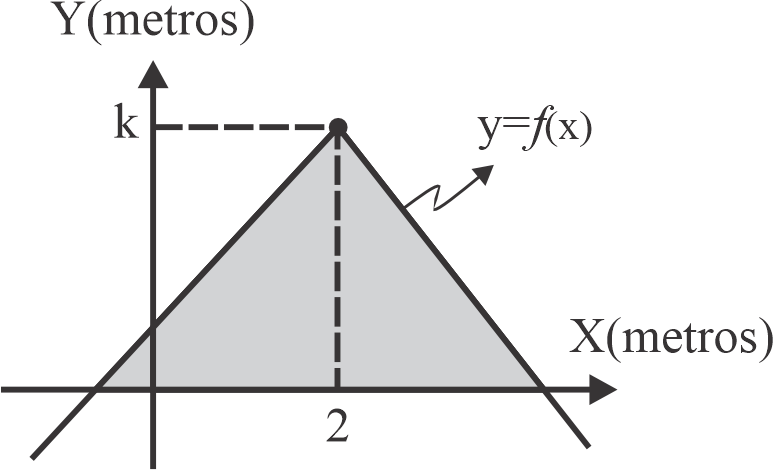
\includegraphics[width=4.5cm]{imagenes/CEPRE-UNA2024-I/etapa2/ing/alg1c24-I.png}
	\end{center}
	
	Halle el área de la región sombreada en metros cuadrados.
	
	\begin{enumerate}[label=\alph*)]
		\item $3\ m^2$
		\item $6\ m^2$
		\item $9\ m^2$
		\item $12\ m^2$
		\item $15\ m^2$
	\end{enumerate}
	\textbf{Respuesta correcta:} c)
	
	\vspace{2mm}
	\textbf{Solucionario:}
	
	$y-k=-|x-h|$ función valor absoluto que se abre hacia abajo.
	
	$\Rightarrow k=3$ y $h=2$.
	
	$|x-2|=-(y-3)$
	
	Si $y=0$:
	
	$\Rightarrow x=5 \quad \text{y} \quad x=-1$
	
	Entonces la base es:
	
	$5-(-1)=6$
	
	La altura es:
	
	$3$
	
	$A=\dfrac{6(3)}{2}=9\ m^2$
	
	\fbox{$A=9\ m^2$}
	
	\vspace{6mm}
	
	\item Halle el dominio de la función.
	
	$f(x)=\log_{4}\left[\log_{1/2}(\log_{3}x)\right]$
	
	\begin{enumerate}[label=\alph*)]
		\item $[-1;3]$
		\item $[1;3]$
		\item $\langle 1;3\rangle$
		\item $\langle 0;+\infty\rangle$
		\item $\langle 2;3\rangle$
	\end{enumerate}
	\textbf{Respuesta correcta:} c)
	
	\vspace{2mm}
	\textbf{Solucionario:}
	
	$\log_{1/2}(\log_3 x)>0$
	
	$\log_3 x<\left(\dfrac{1}{2}\right)^0$ y \quad $\log_3 x>0$
	
	$\log_3 x<1$ y \quad $x>1$
	
	$X<3$
	
	$\therefore \ D_f=\langle 1,3\rangle$
	
	\fbox{$D_f=\langle 1,3\rangle$}
	
	\vspace{6mm}
	
	\item Calcule el área del mayor rectángulo que tiene su base inferior en el eje $x$ y con dos vértices en la curva $y=12-x^2$
	
	\begin{enumerate}[label=\alph*)]
		\item $42\ u^2$
		\item $22\ u^2$
		\item $32\ u^2$
		\item $12\ u^2$
		\item $14\ u^2$
	\end{enumerate}
	\textbf{Respuesta correcta:} c)
	
	\vspace{2mm}
	\textbf{Solucionario:}
	
	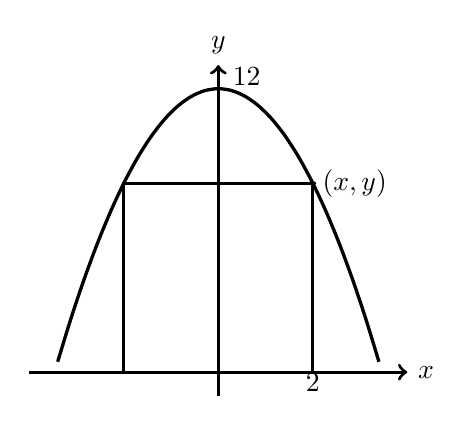
\begin{tikzpicture}[scale=0.6, yscale=0.50]
		\draw[->, very thick] (-4,0) -- (4,0) node[right] {$x$};
		\draw[->, very thick] (0,-1) -- (0,13) node[above] {$y$};
		\draw[domain=-3.4:3.4,smooth,variable=\x,very thick] plot ({\x},{12-\x*\x});
		\draw[very thick] (-2,0) rectangle (2,8);
		\fill (2,8) circle (2.2pt) node[right] {$(x,y)$};
		\node at (0.6,12.5) {$12$};
		\node at (2,-0.45) {$2$};
	\end{tikzpicture}

	
	$A(x)=A=2x\cdot y=2x(12-x^2)$
	
	$A(x)=24x-2x^3$
	
	$A'(x)=24-6x^2 \Rightarrow x=2$
	
	$A''(x)=-12x$
	
	$A''(2)<0 \rightarrow A_{\max}(2)=32$
	
	\fbox{$A_{\max}=32\ u^2$}
	
	\vspace{6mm}
	
	\item Determine la variación de la expresión:
	
	$$E=\dfrac{x^2+y^2}{x^2+xy+y^2}, \quad \text{si } x,y\in \mathbb{R}^{+}$$
	
	\begin{enumerate}[label=\alph*)]
		\item $E\in \left[\dfrac{2}{3};1\right]$
		\item $E\in \left[\dfrac{2}{3};+\infty\right\rangle$
		\item $E\in \left[\dfrac{2}{3};1\right\rangle$
		\item $E\in \left\langle 0;\dfrac{2}{3}\right]$
		\item $E\in \left\langle \dfrac{2}{3};1\right\rangle$
	\end{enumerate}
	\textbf{Respuesta correcta:} c)
	
	\vspace{2mm}
	\textbf{Solucionario:}
	
	$x^2+y^2\geq 2xy$
	
	$3(x^2+y^2)\geq 2x^2+2xy+2y^2$
	
	$\dfrac{x^2+y^2}{x^2+xy+y^2}\geq \dfrac{2}{3}$
	
	Además, como $xy>0$:
	
	$x^2+xy+y^2>x^2+y^2$
	
	$\therefore 1>\dfrac{x^2+y^2}{x^2+xy+y^2}$
	
	$\therefore E\in \left[\dfrac{2}{3},1\right\rangle$
	
	\fbox{$E\in \left[\dfrac{2}{3},1\right\rangle$}
	
	\vspace{6mm}
	
\end{enumerate}





\subsection*{Geometría}

\begin{enumerate}[resume]
	
	\item En la figura, si $AB=5\sqrt{2}$, halle $x$.
	
	\begin{center}
		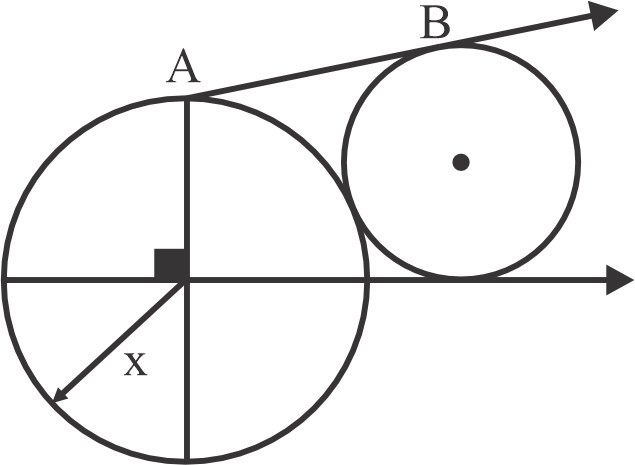
\includegraphics[width=4cm]{imagenes/CEPRE-UNA2024-I/etapa2/ing/geo1c24-I.png}
	\end{center}
	
	\begin{enumerate}[label=\alph*)]
		\item $\sqrt{2}$
		\item $3$
		\item $4$
		\item $5$
		\item $3\sqrt{2}$
	\end{enumerate}
	\textbf{Respuesta correcta:} d)
	
	\vspace{2mm}
	\textbf{Solucionario:}
	
	\begin{center}
		\begin{minipage}{0.45\textwidth}
		En el $\triangle AO'O$: por el teorema de Euclides.

		$(x+r)^2=\left(\sqrt{50+r^2}\right)^2+x^2-2x(x-r)$
		
		$x^2+2xr+r^2=50+r^2+x^2-2x^2+2xr$
		
		$2x^2=50$
		
		$x^2=25$
		
		$x=5$
		
		\fbox{$x=5$}
			\vspace{6mm}
		\end{minipage}
		\hfill
		\begin{minipage}{0.45\textwidth}
			\centering
			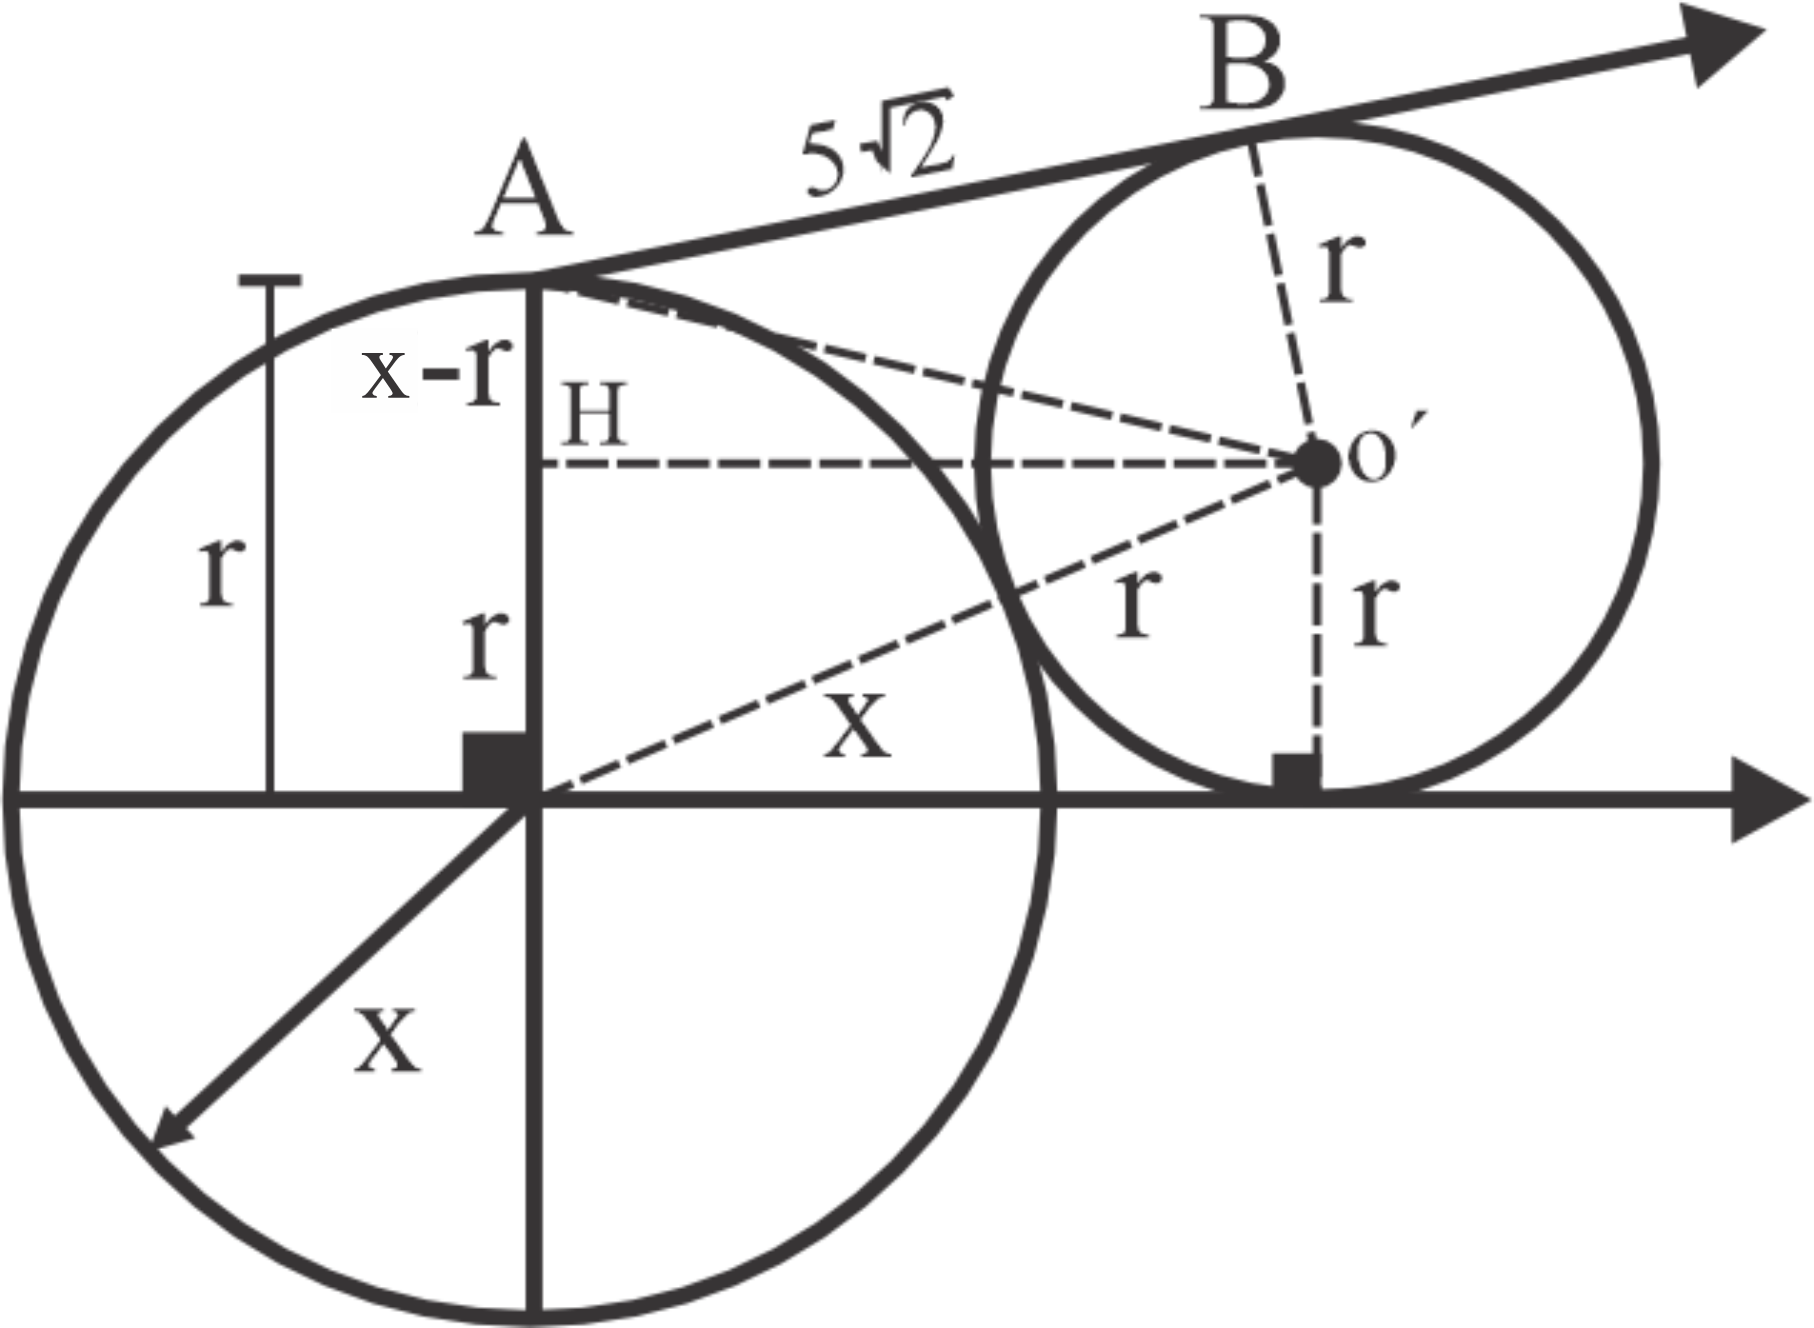
\includegraphics[width=4cm]{imagenes/CEPRE-UNA2024-I/etapa2/ing/geo1c24-Ir.png}
		\end{minipage}
	\end{center}
	
	
	
	\vspace{6mm}
	
	\item Roberto tiene una tabla en forma de triángulo equilátero, pero se da cuenta de que es demasiado grande, por lo que decide hacerle un corte para obtener un triángulo equilátero más pequeño. Calcule el perímetro de la tabla inicial.
	
	\begin{center}
		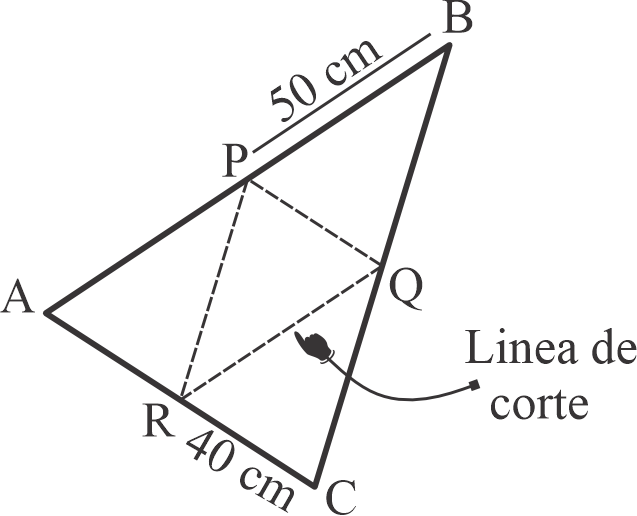
\includegraphics[width=4cm]{imagenes/CEPRE-UNA2024-I/etapa2/ing/geo2c24-I.png}
	\end{center}
	
	\begin{enumerate}[label=\alph*)]
		\item $210\ cm$
		\item $230\ cm$
		\item $250\ cm$
		\item $270\ cm$
		\item $280\ cm$
	\end{enumerate}
	\textbf{Respuesta correcta:} d)
	
	\vspace{2mm}
	\textbf{Solucionario:}
	
	
	
	
	\begin{center}
		\begin{minipage}{0.45\textwidth}
	
		Complemento ángulos, de donde:
		
		$\triangle APR\cong\triangle CRQ\cong\triangle BQP$ $(ALA)$
		
		Luego, $AR=CQ=PB=50\ cm$
		
		El lado del triángulo $\triangle ABC$ mide $90\ cm$
		
		Luego: perímetro $\triangle ABC=90+90+90$
		
		\fbox{$P_{\triangle ABC}=270\ cm$}
			\vspace{6mm}
		\end{minipage}
		\hfill
		\begin{minipage}{0.45\textwidth}
			\centering
			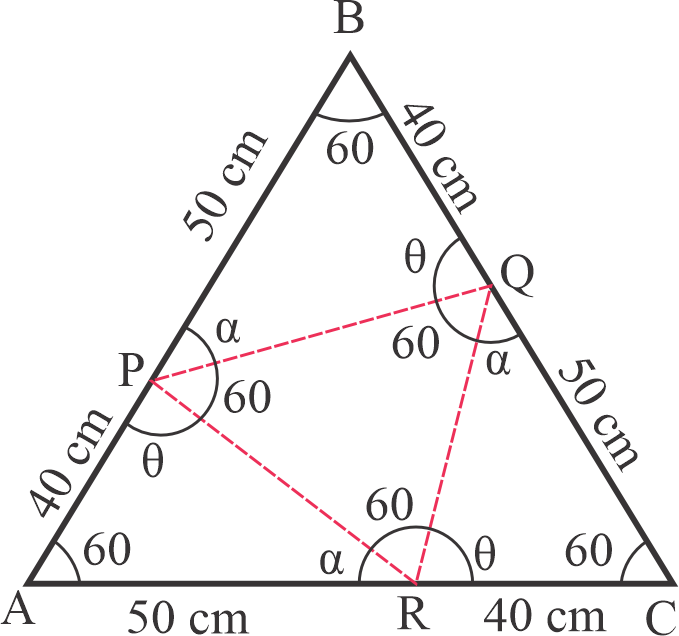
\includegraphics[width=4.2cm]{imagenes/CEPRE-UNA2024-I/etapa2/ing/geo2c24-Ir.png}
		\end{minipage}
	\end{center}
	
	
	
	
	
	
	\vspace{6mm}
	
	\item En la figura, calcule $x$.
	
	\begin{center}
		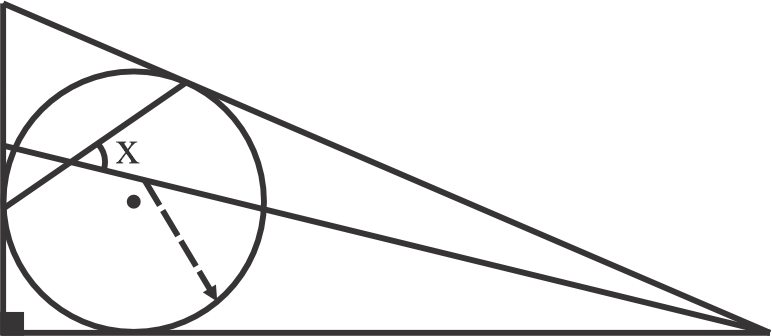
\includegraphics[width=5.2cm]{imagenes/CEPRE-UNA2024-I/etapa2/ing/geo3c24-I.png}
	\end{center}
	
	\begin{enumerate}[label=\alph*)]
		\item $60^\circ$
		\item $45^\circ$
		\item $83^\circ$
		\item $52^\circ$
		\item $74^\circ$
	\end{enumerate}
	\textbf{Respuesta correcta:} b)
	
	\vspace{2mm}
	\textbf{Solucionario:}

	
	\begin{center}
		\begin{minipage}{0.45\textwidth}
			
		En la figura obtenemos que:
		
		$\triangle MBC\cong\triangle MNC$ $(L.A.L)$
		
		
		$m\angle CMN=m\angle CMB=x$
		
		
		$m\angle MNA=m\angle MAB=\theta$
		
		$m\angle BPM=m\angle MNA=\theta$
		
		También del cuadrilátero $APMN$ obtendremos:
		
		$90^\circ+\theta+180^\circ-\theta+180^\circ-2x=360^\circ$
		
		$2x=90^\circ$
		
		
		\fbox{$x=45^\circ$}
			\vspace{6mm}
		\end{minipage}
		\hfill
		\begin{minipage}{0.45\textwidth}
			\centering
			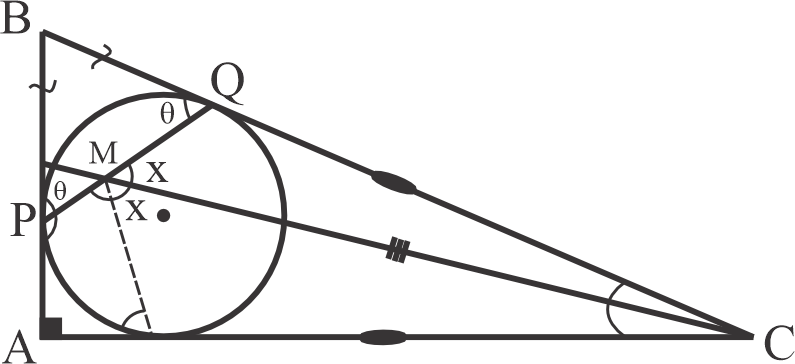
\includegraphics[width=5.2cm]{imagenes/CEPRE-UNA2024-I/etapa2/ing/geo3c24-Ir.png}
		\end{minipage}
	\end{center}
	
	
	
	
	\vspace{6mm}
	
	\item Se tiene dos conos de revolución en donde sus bases se encuentran en una mesa, y de altura $8\ m$ y $4\ m$ respectivamente. Un plano paralelo a la mesa intercepta a los dos conos a la misma altura, generando secciones equivalentes. Calcule el área de dicha sección en $m^2$.
	
	\begin{enumerate}[label=\alph*)]
		\item $12\pi\ m^2$
		\item $14\pi\ m^2$
		\item $16\pi\ m^2$
		\item $18\pi\ m^2$
		\item $25\pi\ m^2$
	\end{enumerate}
	\textbf{Respuesta correcta:} c)
	
	\vspace{2mm}
	\textbf{Solucionario:}
	
	Pide: $S'=$ área del círculo análogo.
	
	$i)$ Semejanza de triángulos en el cono 1:
	
	$\dfrac{r}{6}=\dfrac{8-a}{8}$
	
	$8r=48-6a$ \quad $\cdots (1)$
	
	$8r=24+4r$
	
	$4r=24-6a$
	
	$3a=12-r$ \quad $\cdots (2)$
	
	$ii)$ Semejanza de triángulos en el cono 2:
	
	$\dfrac{r}{12}=\dfrac{4-a}{4}$
	
	$4r=48-12a$
	
	$3a=12-r$ \quad $\cdots (3)$
	
	De $(1)$ y $(2)$:
	
	$12-r=24-4r$
	
	$3r=12$
	
	$r=4$
	
	Por lo tanto,
	
	$S'=\pi r^2=\pi(4)^2$
	
	\fbox{$S'=16\pi\ m^2$}
	
	\vspace{6mm}
	
\end{enumerate}





\subsection*{Trigonometría}

\begin{enumerate}[resume]
	
	\item Desde el pie de un poste, el ángulo de elevación de la punta de un campanario es $26^\circ 30'$, desde la parte superior del poste que tiene $10\ m$ de altura, el ángulo de elevación es $18^\circ 30'$. Halle la distancia entre el poste y el campanario.
	
	\begin{enumerate}[label=\alph*)]
		\item $30\ m$
		\item $60\ m$
		\item $50\ m$
		\item $42\ m$
		\item $45\ m$
	\end{enumerate}
	\textbf{Respuesta correcta:} b)
	
	\vspace{2mm}
	\textbf{Solucionario:}
	
	
	
	
		\begin{center}
		\begin{minipage}{0.45\textwidth}
			
		$18^\circ 30'=\left(\dfrac{\sqrt{37}}{2}\right)^\circ$\\
		
		
		$26^\circ 30'=\left(\dfrac{52}{2}\right)^\circ$\\

		$3x=2x+10$
		
		$x=10$
		
		distancia $=6x$
		
		$=6(10)$
		
		\fbox{$=60\ m$}
			\vspace{6mm}
		\end{minipage}
		\hfill
		\begin{minipage}{0.45\textwidth}
			\centering
			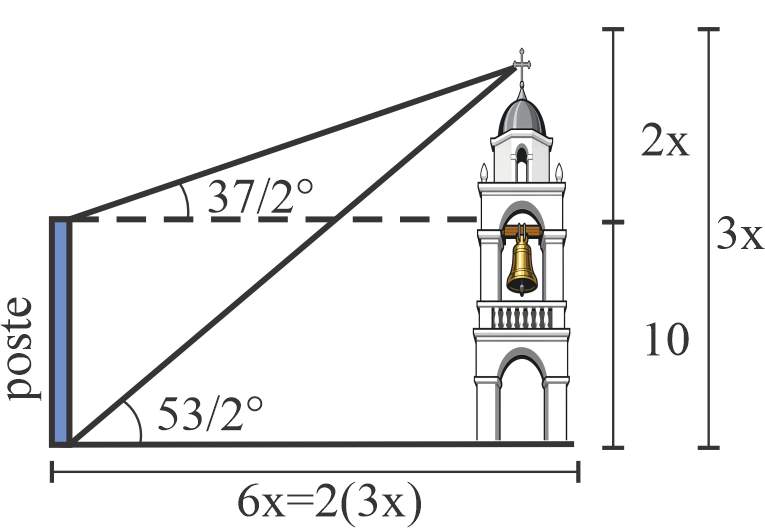
\includegraphics[width=5cm]{imagenes/CEPRE-UNA2024-I/etapa2/ing/trigo1c24-Ir.png}
		\end{minipage}
	\end{center}
	
	
	\vspace{6mm}
	
	\item En la figura, $ABCD$ es un rombo. Calcule $M=\tan\theta+\cot\theta$
	
	\begin{center}
		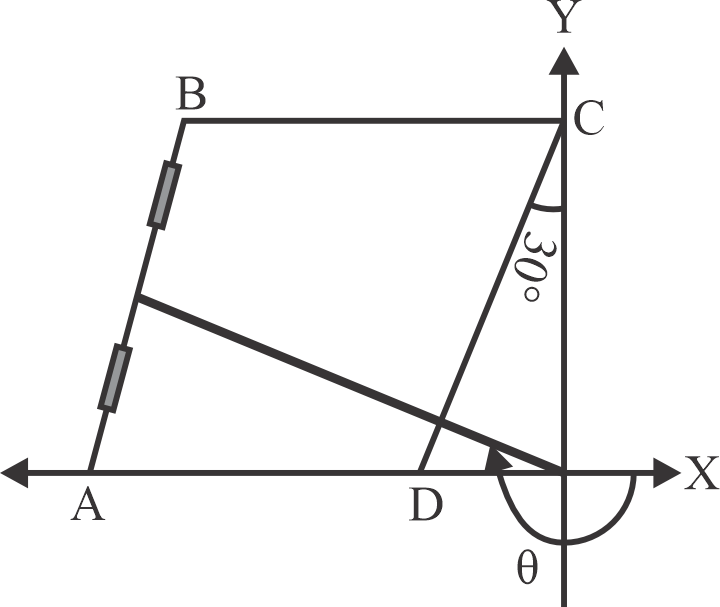
\includegraphics[width=4.8cm]{imagenes/CEPRE-UNA2024-I/etapa2/ing/trigo2c24-I.png}
	\end{center}
	
	\begin{enumerate}[label=\alph*)]
		\item $-\dfrac{25\sqrt{3}}{3}$
		\item $-\dfrac{8\sqrt{3}}{15}$
		\item $-\dfrac{20\sqrt{3}}{3}$
		\item $-\dfrac{28\sqrt{3}}{15}$
		\item $-\dfrac{28\sqrt{3}}{3}$
	\end{enumerate}
	\textbf{Respuesta correcta:} d)
	
	\vspace{2mm}
	\textbf{Solucionario:}
	
	
	\begin{center}
		\begin{minipage}{0.45\textwidth}
			
		$AB=BC=CD=AD$\\

		$\tan\theta+\cot\theta=-\dfrac{\sqrt{3}}{5}-\dfrac{5}{\sqrt{3}}$
		
		$=-\left(\dfrac{\sqrt{3}}{5}+\dfrac{5}{\sqrt{3}}\right)$\\
		
		$=-\left(\dfrac{3+25}{5\sqrt{3}}\right)$\\
		
		$=-\dfrac{28}{5\sqrt{3}}$
		
		\fbox{$\tan\theta+\cot\theta=-\dfrac{28\sqrt{3}}{15}$}
			\vspace{6mm}
		\end{minipage}
		\hfill
		\begin{minipage}{0.45\textwidth}
			\centering
			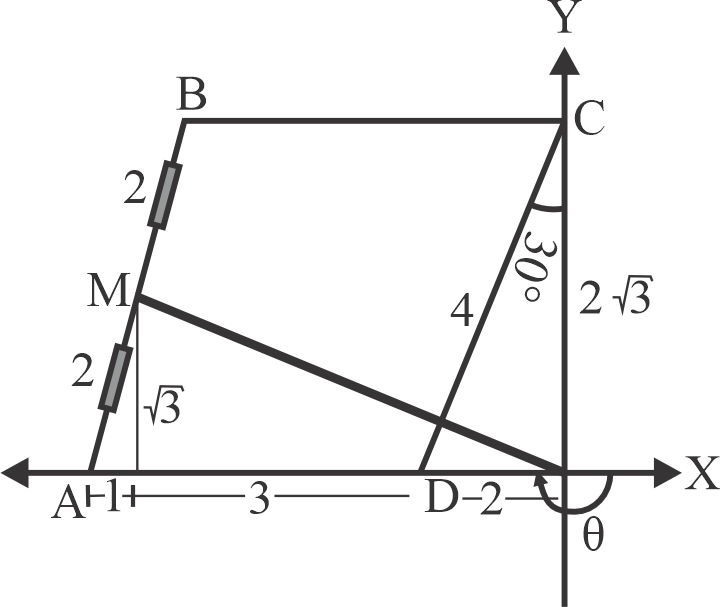
\includegraphics[width=4.8cm]{imagenes/CEPRE-UNA2024-I/etapa2/ing/trigo2c24-Ir.png}
		\end{minipage}
	\end{center}
	
	
	
	\vspace{6mm}
	
	\item Si $\theta\in\left[\dfrac{7\pi}{6},\dfrac{11\pi}{6}\right]$, determine la suma del máximo y mínimo valor de:
	
	$M=\sqrt{3}\cot\theta+3$
	
	\begin{enumerate}[label=\alph*)]
		\item $2$
		\item $3$
		\item $4$
		\item $5$
		\item $6$
	\end{enumerate}
	\textbf{Respuesta correcta:} e)
	
	\vspace{2mm}
	\textbf{Solucionario:}
	
	Analicemos en la circunferencia unitaria:
	
	$\theta\in\left[\dfrac{7\pi}{6},\dfrac{11\pi}{6}\right]\ ;\ \left[\dfrac{7\pi}{6},\dfrac{11\pi}{6}\right]=[210^\circ,330^\circ]$
	
	$\cot 210^\circ=\cot 30^\circ=\sqrt{3}$
	
	$\cot 330^\circ=-\cot 30^\circ=-\sqrt{3}$
	
	$210^\circ\leq \theta\leq 330^\circ$
	
	$\cot 210^\circ\geq \cot\theta\geq \cot 330^\circ$
	
	$\sqrt{3}\geq \cot\theta\geq -\sqrt{3}$
	
	$\sqrt{3}\cdot\sqrt{3}\geq \sqrt{3}\cot\theta\geq -\sqrt{3}(\sqrt{3})$
	
	$3\geq \sqrt{3}\cot\theta\geq -3$
	
	$3+3\geq \sqrt{3}\cot\theta+3\geq -3+3$
	
	$6\geq M\geq 0$
	
	Suma:
	
	\fbox{$6+0=6$}
	
	\vspace{6mm}
	
	\item A partir del triángulo $ABC$ de perímetro $30\ m$, reduzca la expresión:
	
	$M=(a+b)\cos C+(b+c)\cos A+(a+c)\cos B$
	
	\begin{enumerate}[label=\alph*)]
		\item $32\ m$
		\item $28\ m$
		\item $34\ m$
		\item $30\ m$
		\item $27\ m$
	\end{enumerate}
	\textbf{Respuesta correcta:} d)
	
	\vspace{2mm}
	\textbf{Solucionario:}
	
	
\begin{tikzpicture}[scale=0.6]
	
	% Vértices
	\coordinate (A) at (0,0);
	\coordinate (B) at (7,0);
	\coordinate (C) at (3.2,4.2);
	\coordinate (D) at (3.2,0);
	
	% Triángulo
	\draw[very thick] (A) -- (C) -- (B) -- cycle;
	
	% Altura
	\draw[very thick, red] (C) -- (D);
	
	% Etiquetas de lados
	\node[left] at ($(A)!0.55!(C)$) {$b$};
	\node[right] at ($(B)!0.55!(C)$) {$a$};
	\node[below] at ($(A)!0.25!(D)$) {$b\cos A$};
	\node[below] at ($(D)!0.5!(B)$) {$a\cos B$};
	\node[below] at ($(A)!0.5!(B)$) {$c$};
	
	% Ángulo recto
	\draw[very thick] ($(D)+(0,0.28)$) -- ($(D)+(0.28,0.28)$) -- ($(D)+(0.28,0)$);
	
	% Nombres de vértices
	\node[below left] at (A) {$A$};
	\node[below right] at (B) {$B$};
	\node[above] at (C) {$C$};
	
\end{tikzpicture}

	
	$c=b\cos A+a\cos B$
	
	$a=b\cos C+c\cos B$
	
	$b=a\cos C+c\cos A$
	
	$M=a\cos C+b\cos C+b\cos A+c\cos A+a\cos B+c\cos B$
	
	$=a\cos C+c\cos A+b\cos C+c\cos B+b\cos A+a\cos B$
	
	$=b+a+c$
	
	$=a+b+c$
	
	Como el perímetro del triángulo es $30\ m$:
	
	\fbox{$M=30\ m$}
	
	\vspace{6mm}
	
\end{enumerate}



\subsection*{Física}

\begin{enumerate}[resume]
	
	\item En la figura, halle el ángulo $\theta$ que determina el equilibrio de la barra homogénea que está sujeta a una cuerda de masa despreciable.
	
	\begin{center}
		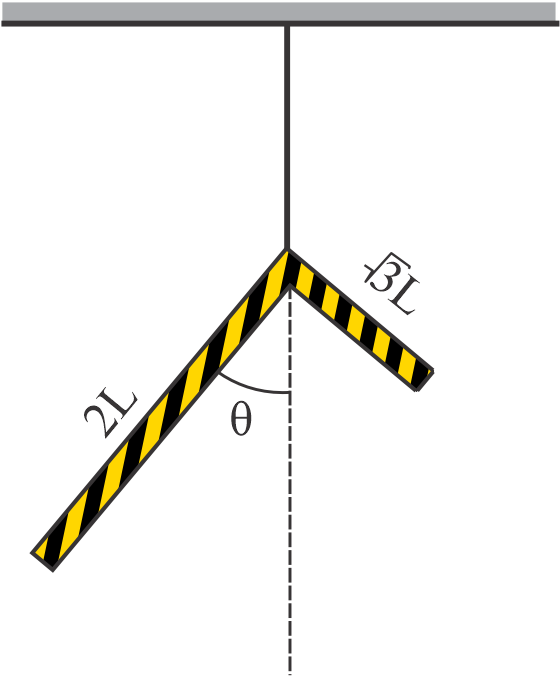
\includegraphics[width=2.8cm]{imagenes/CEPRE-UNA2024-I/etapa2/ing/fisica1c24-I.png}
	\end{center}
	
	
	\begin{enumerate}[label=\alph*)]
		\item $30^\circ$
		\item $37^\circ$
		\item $45^\circ$
		\item $53^\circ$
		\item $60^\circ$
	\end{enumerate}
	\textbf{Respuesta correcta:} b)
	
	\vspace{2mm}
	\textbf{Solucionario:}
	
	$M_1=M_2$
	
	$W_1d_1=W_2d_2$
	
	$k\,2L\cdot \sqrt{3}L\sen\theta=k\sqrt{3}L\cdot \dfrac{\sqrt{3}}{2}L\cos\theta$
	
	$\sen\theta=\dfrac{\sqrt{3}\sqrt{3}}{2(2)}\cos\theta$
	
	$\tan\theta=\dfrac{3}{4}$
	
	\fbox{$\theta=37^\circ$}
	
	\vspace{6mm}
	
	\item Determine la cantidad de calor necesario que se debe suministrar a $500\ g$ de hielo que se encuentra a $0^\circ C$ para convertirlo en agua a $20^\circ C$.
	
	\begin{enumerate}[label=\alph*)]
		\item $80\ \text{kcal}$
		\item $70\ \text{kcal}$
		\item $60\ \text{kcal}$
		\item $55\ \text{kcal}$
		\item $50\ \text{kcal}$
	\end{enumerate}
	\textbf{Respuesta correcta:} e)
	
	\vspace{2mm}
	\textbf{Solucionario:}
	
	$Q_t=Q_f+Q$
	
	$\Rightarrow L_f\,m+mc\,(T_f-T_i)$
	
	$\Rightarrow \left(80\dfrac{\text{cal}}{g}\right)(500\,g)+\left(500\,g\right)\left(1\dfrac{\text{cal}}{g^\circ C}\right)(20-0)^\circ C$
	
	$\Rightarrow (40000+10000)\,\text{cal}$
	
	$=50000\,\text{cal}=$\fbox{$50\,\text{kcal}$}
	
	\vspace{6mm}
	
	\item Una plancha eléctrica tiene una potencia de $800\ W$ cuando se conecta a una tensión de $220\ V$. Calcule su potencia de consumo a $110\ V$.
	
	\begin{enumerate}[label=\alph*)]
		\item $110\ W$
		\item $150\ W$
		\item $180\ W$
		\item $200\ W$
		\item $220\ W$
	\end{enumerate}
	\textbf{Respuesta correcta:} d)
	
	\vspace{2mm}
	\textbf{Solucionario:}
	
	$R_{(1)}=R_{(2)}$
	
	$\dfrac{V_1^2}{P_1}=\dfrac{V_2^2}{P_2}$
	
	$\dfrac{(220\,V)^2}{800}=\dfrac{(110)^2}{P_2}$
	
	$P_2=\dfrac{800(110)^2}{(220)^2}\,W$
	
	\fbox{$P_2=200\,W$}
	
	\vspace{6mm}
	
	\item ¿Con qué ángulo se refleja un rayo luminoso en un espejo plano que ha girado $15^\circ$ en sentido horario con respecto al rayo reflejado en el espejo en su posición original?
	
	\begin{enumerate}[label=\alph*)]
		\item $10^\circ$
		\item $20^\circ$
		\item $30^\circ$
		\item $40^\circ$
		\item $50^\circ$
	\end{enumerate}
	\textbf{Respuesta correcta:} c)
	
	\vspace{2mm}
	\textbf{Solucionario:}
	
	Nos piden hallar $\beta$
	
	$\theta_i+15^\circ+\theta_i+15^\circ=\theta_i+\theta_i+\beta$
	
	$2\theta_i+30^\circ=2\theta_i+\beta$
	
	\fbox{$30^\circ=\beta$}
	
	\vspace{6mm}
	
\end{enumerate}



\subsection*{Química}

\begin{enumerate}[resume]
	
	\item El increíble Hulk está jugando béisbol, batea una pelota cuya masa es $100\ g$, generando una longitud de onda $(\lambda)$ de $3{,}306\times10^{-26}\ \AA$. ¿A qué distancia llega la pelota en un tiempo de $3$ segundos?
	\begin{enumerate}[label=\alph*)]
		\item $5\ Km$
		\item $3\ Km$
		\item $60\ Km$
		\item $6\ Km$
		\item $400\ m$
	\end{enumerate}
	\textbf{Respuesta correcta:} d)
	
	\vspace{2mm}
	\textbf{Solucionario:}\\[1mm]
	
	$m=100\ g=10^2g\cdot\dfrac{1\ kg}{10^3g}=10^{-1}\ kg$
	
	$t=3\ s$
	
	$\lambda=3{,}306\times10^{-26}\ \AA\times\dfrac{10^{-10}\ m}{1\ \AA}=3{,}31\times10^{-36}\ m$
	
	$\lambda=\dfrac{h}{mu}$
	
	$u=\dfrac{h}{m\lambda}=\dfrac{6{,}62\times10^{-34}\ J\cdot s}{(10^{-1}\ kg)(3{,}31\times10^{-36}\ m)}$
	
	$u=\dfrac{6{,}62\times10^{-34}}{3{,}31\times10^{-37}}=2\times10^3\ \dfrac{m}{s}$
	
	$d=e=V\times t=(2\times10^3\ \dfrac{m}{s})(3\ s)=6\times10^3\ m$
	
	$=6\times10^3\ m\times\dfrac{1\ Km}{10^3\ m}=$\fbox{$6\ Km$}
	
	\vspace{6mm}
	
	\item ¿Cuál de los iones está mal nombrado?
	
	I. $\mathrm{ClO_4^-}$ Perclorato
	
	II. $\mathrm{PO_3^{3-}}$ Fosfato
	
	III. $\mathrm{CO_2^{2-}}$ Carbonato
	
	IV. $\mathrm{Cl^-}$ Cloruro
	
	V. $\mathrm{HSO_4^-}$ Bisulfato
	
	\begin{enumerate}[label=\alph*)]
		\item I y IV
		\item II y V
		\item Solo III
		\item IV y II
		\item Solo V
	\end{enumerate}
	\textbf{Respuesta correcta:} b)
	
	\vspace{2mm}
	\textbf{Solucionario:}\\[1mm]
	
	$(\mathrm{Cl^{+7}O_4^{2-}})^{1-}$ \quad perclorato \quad ok
	
	$(\mathrm{P^{+5}O_3^{2-}})^{1-}$ \quad fosfato \quad ok
	
	$(\mathrm{C^{+4}O_2^{2-}})$ \quad carbonato \quad no
	
	$\mathrm{Cl^{1-}}$ \qquad cloruro \quad ok
	
	$(\mathrm{H^{+1}S^{+6}O_4^{2-}})^{1-}$ \quad bisulfato \quad ok

	
	\vspace{6mm}
	
	\item Un gas ocupa un volumen de $1000\ mL$, a una temperatura de ``$X$'' $^\circ K$ y una presión de ``$P$'' atm. Si la presión disminuye a la mitad y la temperatura se duplica ¿qué volumen en mL ocupa el gas?
	\begin{enumerate}[label=\alph*)]
		\item $400$
		\item $4000$
		\item $4$
		\item $440$
		\item $800$
	\end{enumerate}
	\textbf{Respuesta correcta:} b)
	
	\vspace{2mm}
	\textbf{Solucionario:}\\[1mm]
	
	$V_1=1000\ mL$
	
	$T_1=X^\circ K$
	
	$P_1=P\ atm$
	
	$V_2=?$
	
	$T_2=2X^\circ K$
	
	$P_2=\dfrac{P}{2}\ atm$
	
	$\dfrac{P_1V_1}{T_1}=\dfrac{V_2P_2}{T_2}$
	
	$V_2=\dfrac{P_1V_1T_2}{P_2T_1}=\dfrac{(P)(1000\ mL)(2X)}{\left(\dfrac{P}{2}\right)X}$
	
	$V_2=4\times1000\ mL=$\fbox{$4000\ mL$}
	
	\vspace{6mm}
	
	\item El acetominofen es una amida usada para calmar el dolor; es decir como analgésico; y su estructura es:
	
	\begin{center}
		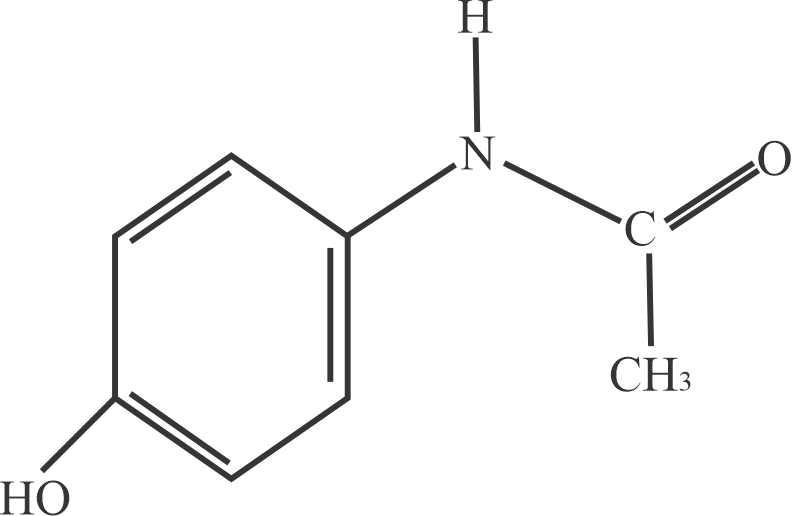
\includegraphics[width=4cm]{imagenes/CEPRE-UNA2024-I/etapa2/ing/quimica4c24-I.png}
	\end{center}
	
	Determine su peso molecular en g/mol
	\begin{enumerate}[label=\alph*)]
		\item $126$
		\item $96$
		\item $120$
		\item $151$
		\item $171$
	\end{enumerate}
	\textbf{Respuesta correcta:} d)
	
	\vspace{2mm}
	\textbf{Solucionario:}\\[1mm]
	
	$C=8\times12=96$
	
	$H=1\times9=9$
	
	$O=2\times16=32$
	
	$N=1\times14=14$
	
	$96+9+32+14=$\fbox{$151$}
	
	\vspace{6mm}
	
\end{enumerate}








\subsection*{Biología y Anatomía}

\begin{enumerate}[resume]
	
	\item El corazón tiene como función recibir y expulsar la sangre mediante los vasos sanguíneos. ¿Cuál es el vaso sanguíneo que sale del ventrículo derecho y transporta la sangre venosa hacia los pulmones?
	\begin{enumerate}[label=\alph*)]
		\item Vena cava superior
		\item Vena cava inferior
		\item Vena pulmonar
		\item Arteria pulmonar
		\item Arteria aorta
	\end{enumerate}
	\textbf{Respuesta correcta:} d)
	
	\vspace{2mm}
	\textbf{Solucionario:}\\[1mm]
	El vaso que lleva la sangre venosa hacia los pulmones es la \textbf{arteria pulmonar}.
	
	\vspace{6mm}
	
	\item Los mamíferos acuáticos respiran por:
	\begin{enumerate}[label=\alph*)]
		\item sacos pulmonares.
		\item branquias.
		\item vejiga natatoria.
		\item piel.
		\item pulmones.
	\end{enumerate}
	\textbf{Respuesta correcta:} e)
	
	\vspace{2mm}
	\textbf{Solucionario:}\\[1mm]
	Los mamíferos, aunque sean acuáticos, respiran por \textbf{pulmones}.
	
	\vspace{6mm}
	
\end{enumerate}

\subsection*{Psicología y Filosofía}

\begin{enumerate}[resume]

	
	\item Al comparar dos prendas, notamos una pequeña diferencia que da lugar a un cambio en la percepción. Este fenómeno se conoce como umbral:
	\begin{enumerate}[label=\alph*)]
		\item superior.
		\item mínimo.
		\item diferencial.
		\item máximo.
		\item sensorial.
	\end{enumerate}
	\textbf{Respuesta correcta:} c)
	
	\vspace{2mm}
	\textbf{Solucionario:}\\[1mm]
	La mínima diferencia perceptible entre dos estímulos se llama \textbf{umbral diferencial}.
	
	\vspace{6mm}
	
	\item Es el pensamiento multidireccional que se aplica en la solución del problema en muchas direcciones posibles. Se relaciona con la creatividad.
	\begin{enumerate}[label=\alph*)]
		\item Lógico
		\item No lógico
		\item Convergente
		\item Divergente
		\item Probabilístico
	\end{enumerate}
	\textbf{Respuesta correcta:} d)
	
	\vspace{2mm}
	\textbf{Solucionario:}\\[1mm]
	El pensamiento que explora varias posibilidades y alternativas es el \textbf{divergente}.
	
	\vspace{6mm}
	
	\item Juan, al terminar sus estudios universitarios, tendrá que sustentar su tesis. Esto implica que argumentará y explicará sus conclusiones con respecto a un tema. Entonces, su aprendizaje es:
	\begin{enumerate}[label=\alph*)]
		\item motor.
		\item actitudinal.
		\item social.
		\item instrumental.
		\item cognitivo.
	\end{enumerate}
	\textbf{Respuesta correcta:} e)
	
	\vspace{2mm}
	\textbf{Solucionario:}\\[1mm]
	Sustentar una tesis exige comprender, analizar, argumentar y explicar; eso corresponde al aprendizaje \textbf{cognitivo}.
	
	\vspace{6mm}
	
	\item El conocimiento científico es sistemático porque:
	
	\begin{enumerate}[label=\alph*)]
		\item cuestiona a otros conocimientos.
		\item consiste en una organización de leyes y teorías.
		\item está sujeto a un cambio constante.
		\item siempre problematiza sobre ciertos fenómenos.
		\item tiende a reflejar objetivamente la realidad.
	\end{enumerate}
	\textbf{Respuesta correcta:} b)
	
	\vspace{2mm}
	\textbf{Solucionario:}\\[1mm]
	Es sistemático porque organiza sus contenidos en un \textbf{conjunto ordenado de leyes y teorías}.
	
	\vspace{6mm}
	
\end{enumerate}

\subsection*{Geografía}

\begin{enumerate}[resume]

	
	\item Es la corriente marina que forma parte del proceso de circulación mayor del sector sur del Océano Pacífico y que se desplaza en sentido antihorario.
	\begin{enumerate}[label=\alph*)]
		\item Corriente Peruana
		\item Contracorriente Ecuatorial
		\item Corriente del Niño
		\item Corriente Australiana
		\item Corriente Cálida o Boreal
	\end{enumerate}
	\textbf{Respuesta correcta:} a)
	
	\vspace{2mm}
	\textbf{Solucionario:}\\[1mm]
	La corriente que integra la circulación del Pacífico Sur es la \textbf{Corriente Peruana}.
	
	\vspace{6mm}
	
	\item Es la parte visible dentro de la estructura solar de donde proviene la mayor parte de energía luminosa y calorífica que recibe la tierra:
	\begin{enumerate}[label=\alph*)]
		\item Corona
		\item Fotosfera
		\item Cabellera
		\item Núcleo
		\item Cromósfera
	\end{enumerate}
	\textbf{Respuesta correcta:} b)
	
	\vspace{2mm}
	\textbf{Solucionario:}\\[1mm]
	La parte visible del Sol es la \textbf{fotosfera}.
	
	\vspace{6mm}
	
\end{enumerate}

\subsection*{Historia}

\begin{enumerate}[resume]
	
	\item El Ministerio de Desarrollo e Inclusión Social, encargado de mejorar la calidad de vida de los peruanos en extrema pobreza y fomentar la equidad, proteger a poblaciones vulnerables y en estado de abandono, fue creado durante el gobierno de:
	\begin{enumerate}[label=\alph*)]
		\item Valentín Paniagua Corazao.
		\item Alberto Fujimori Fujimori.
		\item Alejandro Toledo Manrique.
		\item Fernando Belaunde Terry.
		\item Ollanta Humala Tasso.
	\end{enumerate}
	\textbf{Respuesta correcta:} e)
	
	\vspace{2mm}
	\textbf{Solucionario:}\\[1mm]
	El MIDIS fue creado durante el gobierno de \textbf{Ollanta Humala Tasso}.
	
	\vspace{6mm}
	
	\item Es la cultura que utilizó el barro, la quincha y el adobe en la arquitectura y cuya capital fue Cahuachi.
	\begin{enumerate}[label=\alph*)]
		\item Moche
		\item Chimú
		\item Paracas
		\item Tiahuanaco
		\item Nasca
	\end{enumerate}
	\textbf{Respuesta correcta:} e)
	
	\vspace{2mm}
	\textbf{Solucionario:}\\[1mm]
	Cahuachi fue el principal centro ceremonial de la cultura \textbf{Nasca}.
	
	\vspace{6mm}
	
\end{enumerate}

\subsection*{Educación Cívica}

\begin{enumerate}[resume]
	
	\item Durante la \rule{2cm}{0.4pt} se reconocen los derechos humanos de primera generación.
	\begin{enumerate}[label=\alph*)]
		\item creación de la ONU
		\item primera guerra mundial
		\item revolución francesa
		\item segunda guerra mundial
		\item revolución inglesa
	\end{enumerate}
	\textbf{Respuesta correcta:} c)
	
	\vspace{2mm}
	\textbf{Solucionario:}\\[1mm]
	Los derechos de primera generación se vinculan con la \textbf{Revolución francesa}.
	
	\vspace{6mm}
	
	\item En el testamento, se nombra a una persona natural o jurídica elegida por el testador para que cumpla o ejecute lo dispuesto en el documento. Se refiere:
	\begin{enumerate}[label=\alph*)]
		\item al tutor.
		\item al curador.
		\item al albacea.
		\item a los padrinos.
		\item a toda la familia.
	\end{enumerate}
	\textbf{Respuesta correcta:} c)
	
	\vspace{2mm}
	\textbf{Solucionario:}\\[1mm]
	La persona encargada de ejecutar lo dispuesto en el testamento es el \textbf{albacea}.
	
	\vspace{6mm}
	
\end{enumerate}

\subsection*{Economía}

\begin{enumerate}[resume]
	
	\item ¿Qué escuela económica sostiene que la riqueza de una nación está determinada por la cantidad de oro y plata que posee?
	\begin{enumerate}[label=\alph*)]
		\item Monetarista
		\item Keynesiana
		\item Neoclásica
		\item Mercantilista
		\item Socialista
	\end{enumerate}
	\textbf{Respuesta correcta:} d)
	
	\vspace{2mm}
	\textbf{Solucionario:}\\[1mm]
	La escuela que identifica la riqueza con la acumulación de metales preciosos es la \textbf{mercantilista}.
	
	\vspace{6mm}
	
	\item En la apertura de un mercado de abastos en la ciudad de Puno, participaron gran número de vendedores, debido a la inclemencia del tiempo hubo un solo comprador. ¿A qué tipo de mercado de competencia corresponde?
	\begin{enumerate}[label=\alph*)]
		\item Mercado mixto
		\item Mercado de capitales
		\item Mercado de monopolio
		\item Mercado de oligopolio
		\item Mercado de monopsonio
	\end{enumerate}
	\textbf{Respuesta correcta:} e)
	
	\vspace{2mm}
	\textbf{Solucionario:}\\[1mm]
	Muchos vendedores y un solo comprador corresponden a un \textbf{monopsonio}.
	
	\vspace{6mm}
	
\end{enumerate}

\subsection*{Comunicación}

\begin{enumerate}[resume]
	
	\item Una oración contiene sujeto y predicado. El sujeto identifica al ser u objeto. El predicado expresa la acción o estado del ser u objeto. El enunciado utiliza el lenguaje en su función:
	\begin{enumerate}[label=\alph*)]
		\item metalingüística.
		\item fática o de contacto.
		\item apelativa o conativa.
		\item referencial o representativa.
		\item expresiva o emotiva.
	\end{enumerate}
	\textbf{Respuesta correcta:} a)
	
	\vspace{2mm}
	\textbf{Solucionario:}\\[1mm]
	El enunciado habla sobre la estructura de la oración y explica elementos del propio lenguaje; por eso cumple función \textbf{metalingüística}.
	
	\vspace{6mm}
	
	\item El transbordador espacial es una estructura de aluminio cubierto de un sistema aislante que impide que temperaturas mayores a $177^\circ C$ se registren dentro del armazón de aluminio y de la fibra de vidrio. El costo de este tipo de cubierta es de un poco más de $23,7$ metros; y el área total es de $250$ metros cuadrados. El fragmento corresponde a un texto:
	\begin{enumerate}[label=\alph*)]
		\item narrativo.
		\item descriptivo.
		\item argumentativo.
		\item instructivo.
		\item dialógico.
	\end{enumerate}
	\textbf{Respuesta correcta:} b)
	
	\vspace{2mm}
	\textbf{Solucionario:}\\[1mm]
	Presenta características y rasgos de un objeto; por ello es un texto \textbf{descriptivo}.
	
	\vspace{6mm}
	
	\item La cohesión es una propiedad textual que se distingue de las demás porque se centra en el aspecto:
	\begin{enumerate}[label=\alph*)]
		\item sintáctico que ve como una frase u oración se conecta lingüísticamente con otra frase u oración.
		\item semántico que ve como la información se distribuye según el esquema global del texto.
		\item pragmático que ve como se seleccionan las estructuras lingüísticas en función de los componentes relacionales.
		\item intencional que ve el motivo que impulsa el desarrollo del texto en una situación comunicativa concreta.
		\item referencial que ve el modo como la realidad se conecta con la expresión lingüística.
	\end{enumerate}
	\textbf{Respuesta correcta:} a)
	
	\vspace{2mm}
	\textbf{Solucionario:}\\[1mm]
	La cohesión se refiere a los enlaces formales entre oraciones; por eso se centra en el aspecto \textbf{sintáctico}.
	
	\vspace{6mm}
	
	\item Juanita tiene 12 años y, en las mañanas, lava los platos y ayuda a su madre en la cocina. El enunciado utiliza el lenguaje en su función:
	\begin{enumerate}[label=\alph*)]
		\item referencial o representativa.
		\item expresiva o emotiva.
		\item apelativa o conativa.
		\item fática y de contacto.
		\item metalingüística.
	\end{enumerate}
	\textbf{Respuesta correcta:} a)
	
	\vspace{2mm}
	\textbf{Solucionario:}\\[1mm]
	El enunciado brinda información objetiva sobre Juanita; por tanto, la función es \textbf{referencial}.
	
	\vspace{6mm}
	
\end{enumerate}

\subsection*{Literatura}

\begin{enumerate}[resume]
	
	\item Es una característica distintiva de la novela \textit{Cien Años de Soledad} de Gabriel García Márquez.
	\begin{enumerate}[label=\alph*)]
		\item Está narrada en primera persona.
		\item Mezcla la lírica con la prosa.
		\item Uso de un lenguaje prosáico.
		\item Es un gran monólogo interior.
		\item Emplea el tiempo narrativo cíclico.
	\end{enumerate}
	\textbf{Respuesta correcta:} e)
	
	\vspace{2mm}
	\textbf{Solucionario:}\\[1mm]
	Una característica central de la novela es el \textbf{tiempo narrativo cíclico}.
	
	\vspace{6mm}
	
	\item En el cuento \textit{El Caballero Carmelo}, Carmelo era un gallo:
	\begin{enumerate}[label=\alph*)]
		\item bravucón y necio.
		\item luchador pero ridículo.
		\item viejo y achacoso.
		\item furioso y conciliador.
		\item de alcurnia y galante.
	\end{enumerate}
	\textbf{Respuesta correcta:} c)
	
	\vspace{2mm}
	\textbf{Solucionario:}\\[1mm]
	El Caballero Carmelo es presentado como un gallo \textbf{viejo y achacoso}.
	
	\vspace{6mm}
	
\end{enumerate}

\subsection*{Razonamiento Matemático}

\begin{enumerate}[resume]
	
	\item Juan le regala a su hijo Pedro la suma de:
	
	$C=12_{(3)}+23_{(4)}+34_{(5)}+45_{(6)}+\cdots$
	
	$10$ sumandos
	
	Halle dicha cantidad en el sistema decimal.
	\begin{enumerate}[label=\alph*)]
		\item $560$
		\item $561$
		\item $570$
		\item $575$
		\item $580$
	\end{enumerate}
	\textbf{Respuesta correcta:} a)
	
	\vspace{2mm}
	\textbf{Solucionario:}


	Analizamos la forma de cada término de la serie ($T_k$):
	\begin{itemize}
		\item $T_1 = 12_{(3)} = 1(3) + 2 = 5$
		\item $T_2 = 23_{(4)} = 2(4) + 3 = 11$
		\item $T_3 = 34_{(5)} = 3(5) + 4 = 19$
	\end{itemize}
	
	$ T_k = k(k+2) + (k+1) $
	
	$ T_k = k^2 + 2k + k + 1 = k^2 + 3k + 1 $
	
	$ C = \sum_{k=1}^{10} (k^2 + 3k + 1) $
	
	$ C = \sum_{k=1}^{10} k^2 + 3\sum_{k=1}^{10} k + \sum_{k=1}^{10} 1 $
	
	Aplicando las fórmulas de sumas notables:
	\begin{enumerate}
		\item Suma de cuadrados: $\dfrac{10(11)(21)}{6} = 385$
		\item Suma de naturales: $3 \times \dfrac{10(11)}{2} = 3(55) = 165$
		\item Suma de constantes: $1 \times 10 = 10$
	\end{enumerate}
	

	$C = 385 + 165 + 10 =$\fbox{$560$}
	
	\vspace{6mm}
	
	\item En cierto año ocurrió que el primer día de un determinado mes fue lunes, mientras que el último día de dicho mes también fue lunes. ¿Qué fecha cayó el primer jueves del mes posterior?
	\begin{enumerate}[label=\alph*)]
		\item 3 de marzo
		\item 2 de mayo
		\item 4 de marzo
		\item 30 de abril
		\item 24 de junio
	\end{enumerate}
	\textbf{Respuesta correcta:} a)
	
	\vspace{2mm}
	\textbf{Solucionario:}
	
	Si el primer día y el último día de un mes son lunes, entonces el mes tiene $29$ días.
	
	El mes siguiente comienza un martes.
	
	Por tanto, el primer jueves del mes siguiente cae el día:

	
	\fbox{$3$ de marzo}
	
	\vspace{6mm}
	
	\item En el gráfico, $T$ y $P$ son puntos de tangencia. Si $AB=2$, calcule el área de la región sombreada.
	
	\begin{center}
		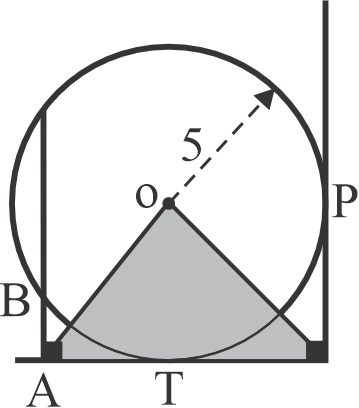
\includegraphics[width=3cm]{imagenes/CEPRE-UNA2024-I/etapa2/ing/rm3c24-I.png}
	\end{center}
	
	\begin{enumerate}[label=\alph*)]
		\item $20\ u^2$
		\item $\dfrac{45}{2}\ u^2$
		\item $25\ u^2$
		\item $\dfrac{49}{2}\ u^2$
		\item $21\ u^2$
	\end{enumerate}
	\textbf{Respuesta correcta:} b)
	
	\vspace{2mm}
	\textbf{Solucionario:}\\[1mm]
	Del gráfico, el radio del círculo es $5$.
	
	Como $AB=2$, en el triángulo rectángulo formado con el radio:
	
	$x^2+3^2=5^2$
	
	$x^2+9=25$
	
	$x=4$
	
	Entonces la base total del triángulo sombreado es:
	
	$AO=AT+TO=4+5=9$
	
	y su altura es el radio:
	
	$5$
	
	Área sombreada:
	
	$A=\dfrac{9\cdot5}{2}=\dfrac{45}{2}\ u^2$
	
	\fbox{$\dfrac{45}{2}\ u^2$}
	
	\vspace{6mm}
	
	\item Se divide un terreno rectangular en parcelas lográndose $108$ parcelas cuadradas de $121\ m^2$ cada una. En cada esquina de las parcelas se coloca un poste, empleándose en total $130$ postes. Halle la diferencia entre el largo y el ancho del terreno rectangular.
	\begin{enumerate}[label=\alph*)]
		\item $44\ m$
		\item $33\ m$
		\item $38\ m$
		\item $52\ m$
		\item $50\ m$
	\end{enumerate}
	\textbf{Respuesta correcta:} b)
	
	\vspace{2mm}
	\textbf{Solucionario:}\\[1mm]
	Cada parcela tiene lado:
	
	$\sqrt{121}=11\ m$
	
	Si el rectángulo tiene $m$ parcelas por un lado y $n$ por el otro:
	
	$mn=108$
	
	y el número de postes es:
	
	$(m+1)(n+1)=130$
	
	$mn+m+n+1=130$
	
	$108+m+n+1=130$
	
	$m+n=21$
	
	Los números que cumplen:
	
	$m=9,\quad n=12$
	
	La diferencia de dimensiones es:
	
	$(12-9)\cdot 11=33\ m$
	
	\fbox{$33\ m$}
	
	\vspace{6mm}
	
	\item Calcule la suma de los 10 primeros términos de la serie
	
	$S=4+12+26+46+\cdots$
	\begin{enumerate}[label=\alph*)]
		\item $1200$
		\item $1110$
		\item $1320$
		\item $1120$
		\item $1000$
	\end{enumerate}
	\textbf{Respuesta correcta:} d)
	
	\vspace{2mm}
	\textbf{Solucionario:}\\[1mm]
	Las diferencias son:
	
	$8,\ 14,\ 20,\dots$
	
	La segunda diferencia es constante, entonces:
	
	$a_n=3n^2-n+2$
	
	Luego:
	
	$S_{10}=\sum_{n=1}^{10}(3n^2-n+2)$
	
	$=3\sum_{n=1}^{10}n^2-\sum_{n=1}^{10}n+2\sum_{n=1}^{10}1$
	
	$=3(385)-55+20$
	
	$=1155-55+20$
	
	\fbox{$= 1120$}
	
	\vspace{6mm}
	
	\item Halle la suma de los elementos de la matriz $10\times10$
	
	\[
	\begin{bmatrix}
		2 & 4 & 6 & \cdots & 18 & 20\\
		4 & 6 & 8 & \cdots & 20 & 22\\
		6 & 8 & 10 & \cdots & 22 & 24\\
		\vdots & \vdots & \vdots & \ddots & \vdots & \vdots\\
		20 & 22 & 24 & \cdots & 36 & 38
	\end{bmatrix}
	\]
	
	\begin{enumerate}[label=\alph*)]
		\item $2200$
		\item $2100$
		\item $2580$
		\item $2000$
		\item $2700$
	\end{enumerate}
	\textbf{Respuesta correcta:} d)
	
	\vspace{2mm}
	\textbf{Solucionario:}\\[1mm]
	El término general es:
	
	$a_{ij}=2(i+j-1)$
	
	Entonces:
	
	$\displaystyle \sum_{i=1}^{10}\sum_{j=1}^{10} a_{ij}
	=\sum_{i=1}^{10}\sum_{j=1}^{10}2(i+j-1)$
	
	$=2\left(10\sum_{i=1}^{10}i+10\sum_{j=1}^{10}j-100\right)$
	
	$=2(10\cdot55+10\cdot55-100)$
	
	$=2(550+550-100)$
	
	$=2(1000)=2000$
	
	\fbox{$2000$}
	
	\vspace{6mm}
	
\end{enumerate}

\subsection*{Razonamiento Verbal}

\begin{enumerate}[resume]
	
	\item Marque la relación incorrecta de sustantivos colectivos:
	\begin{enumerate}[label=\alph*)]
		\item pinar : pinos
		\item clientela : clientes
		\item bosque : árboles
		\item estrellada : estrellas
		\item dentadura : dientes
	\end{enumerate}
	\textbf{Respuesta correcta:} d)
	
	\vspace{2mm}
	\textbf{Solucionario:}\\[1mm]
	``Estrellada'' no es un sustantivo colectivo de estrellas.
	
	La relación incorrecta es:
	
	\fbox{estrellada : estrellas}
	
	\vspace{6mm}
	
	\item La palabra que está implicada en las demás es:
	\begin{enumerate}[label=\alph*)]
		\item legislación.
		\item reglamento.
		\item normativa.
		\item ordenanza.
		\item estatuto.
	\end{enumerate}
	\textbf{Respuesta correcta:} c)
	
	\vspace{2mm}
	\textbf{Solucionario:}\\[1mm]
	La palabra más general, que engloba a las demás, es \textbf{normativa}.
	
	\vspace{6mm}
	
	\item En las oraciones ``Estamos en una estación, en la que los árboles comienzan a florecer y los días se vuelven más largos'' y ``El tren llegó a la estación a tiempo para recoger a los pasajeros que se dirigían a la ciudad''.
	
	¿Cuál es la relación entre las palabras subrayadas?
	\begin{enumerate}[label=\alph*)]
		\item Paronimia
		\item Homografía
		\item Homofonía
		\item Polisemia
		\item Homonimia
	\end{enumerate}
	\textbf{Respuesta correcta:} d)
	
	\vspace{2mm}
	\textbf{Solucionario:}\\[1mm]
	La palabra ``estación'' tiene varios significados relacionados entre sí; eso es \textbf{polisemia}.
	
	\vspace{6mm}
	
	\item El antónimo de la palabra VITUPERABLE es:
	\begin{enumerate}[label=\alph*)]
		\item censurable.
		\item reprochable.
		\item laudable.
		\item condenable.
		\item recusable.
	\end{enumerate}
	\textbf{Respuesta correcta:} c)
	
	\vspace{2mm}
	\textbf{Solucionario:}\\[1mm]
	``Vituperable'' significa digno de reproche; su antónimo es \textbf{laudable}.
	
	\vspace{6mm}
	
	\item PLAN DE REDACCIÓN
	
	Las plantas de interior
	
	I. Hay condiciones ambientales para promover su eficaz desarrollo.
	
	II. Existen diversos tipos de plantas de interior.
	
	III. Su principal función consiste en ser objeto de ornato.
	
	IV. Una de ellas es la adecuada iluminación y
	
	V. Las hay desde las más modestas hasta las más exóticas.
	
	\begin{enumerate}[label=\alph*)]
		\item III -- V -- I -- IV -- II
		\item II -- I -- V -- IV -- III
		\item II -- III -- V -- I -- IV
		\item II -- V -- III -- I -- IV
		\item III -- II -- V -- I -- IV
	\end{enumerate}
	\textbf{Respuesta correcta:} d)
	
	\vspace{2mm}
	\textbf{Solucionario:}\\[1mm]
	Primero se presenta el tema general: II.
	
	Luego se amplía la variedad de las plantas: V.
	
	Después se señala su función principal: III.
	
	Finalmente se mencionan las condiciones para su desarrollo: I, y se precisa una de ellas: IV.
	
	Orden:
	
	II -- V -- III -- I -- IV
	
	\vspace{6mm}
	
	\item Siempre que tomo café en las tardes, no puedo dormir esa noche. Si lo tomo por la mañana, no podré conciliar el sueño hasta medianoche. ¿Cuál de las opciones es necesariamente cierta?
	\begin{enumerate}[label=\alph*)]
		\item Son las dos de la mañana y estoy despierto. Hoy he tomado café.
		\item Tomé café en el desayuno. A las dos de la mañana estaré despierto.
		\item Son las once de la noche y estoy dormido. Hoy no he tomado café.
		\item Estoy despierto a las doce y media de la noche. Hoy he tomado café por la mañana.
		\item Tomé café por la tarde. Dormiré a la medianoche.
	\end{enumerate}
	\textbf{Respuesta correcta:} c)
	
	\vspace{2mm}
	\textbf{Solucionario:}\\[1mm]
	Si toma café en la tarde, no duerme esa noche.
	
	Si lo toma en la mañana, no duerme hasta medianoche.
	
	Entonces, si a las once de la noche está dormido, necesariamente \textbf{no tomó café ese día}.
	
	\vspace{6mm}
\end{enumerate}

\subsection*{Inglés}

\begin{enumerate}[resume]
	
	\item Find the list with the right question words to complete the questions of this conversation.
	
	A: Good morning, sir. \rule{1.5cm}{0.4pt} is your name?
	
	B: My name is Brown.
	
	A: \rule{1.5cm}{0.4pt} did you arrive?
	
	B: At 8:00 o'clock this morning.
	
	A: \rule{1.5cm}{0.4pt} did you come here?
	
	B: I took a taxi.
	
	\begin{enumerate}[label=\alph*)]
		\item What -- Who -- Where
		\item What -- How -- Who
		\item What -- When -- How
		\item What -- Who -- When
		\item What -- Where -- How
	\end{enumerate}
	\textbf{Respuesta correcta:} c)
	
	\vspace{2mm}
	\textbf{Solucionario:}\\[1mm]
	Las preguntas correctas son:
	
	What is your name?
	
	When did you arrive?
	
	How did you come here?
	
	\vspace{6mm}
	
	\item Look at this chart, and choose the right information
	
\begin{center}
	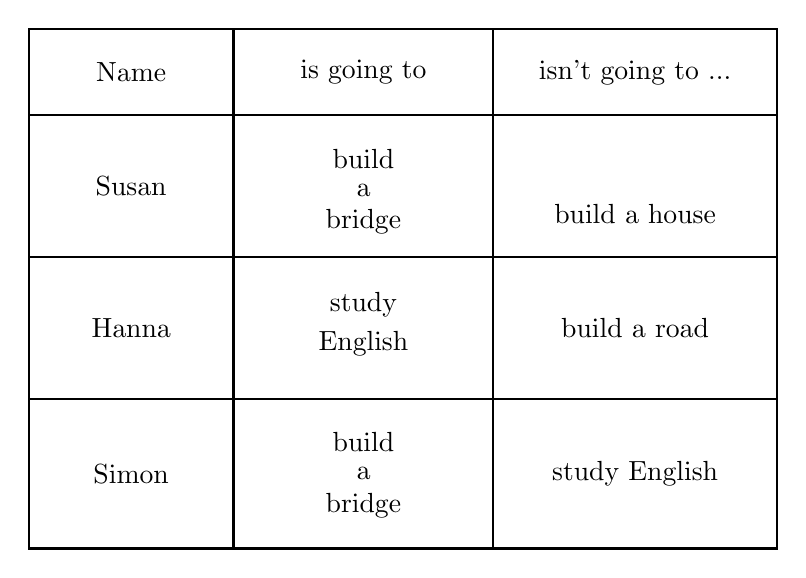
\begin{tikzpicture}
		% marco
		\draw[thick] (0,0) rectangle (9.5,6.6);
		
		% columnas
		\draw[thick] (2.6,0) -- (2.6,6.6);
		\draw[thick] (5.9,0) -- (5.9,6.6);
		
		% filas
		\draw[thick] (0,5.5) -- (9.5,5.5);
		\draw[thick] (0,3.7) -- (9.5,3.7);
		\draw[thick] (0,1.9) -- (9.5,1.9);
		
		% encabezados
		\node at (1.3,6.05) {Name};
		\node at (4.25,6.05) {is going to};
		\node at (7.7,6.05) {isn't going to ...};
		
		% Susan
		\node at (1.3,4.6) {Susan};
		\node at (4.25,4.95) {build};
		\node at (4.25,4.55) {a};
		\node at (4.25,4.15) {bridge};
		\node at (7.7,4.25) {build a house};
		
		% Hanna
		\node at (1.3,2.8) {Hanna};
		\node at (4.25,3.1) {study};
		\node at (4.25,2.6) {English};
		\node at (7.7,2.8) {build a road};
		
		% Simon
		\node at (1.3,0.95) {Simon};
		\node at (4.25,1.35) {build};
		\node at (4.25,0.95) {a};
		\node at (4.25,0.55) {bridge};
		\node at (7.7,0.95) {study English};
	\end{tikzpicture}
\end{center}

	\begin{enumerate}[label=\alph*)]
		\item Susan and Simon are going to build a bridge.
		\item Hanna is going to build a road.
		\item Simon and Susan are going to study English.
		\item Susan and Hanna are going to build a house.
		\item Simon is going to build a road.
	\end{enumerate}
	\textbf{Respuesta correcta:} a)
	
	\vspace{2mm}
	\textbf{Solucionario:}\\[1mm]
	Según la tabla, Susan is going to build a bridge y Simon is going to build a bridge.
	
	Por tanto, la opción correcta es:
	
	\fbox{Susan and Simon are going to build a bridge.}
	
	\vspace{6mm}
	
\end{enumerate}

\subsection*{Quechua y Aimara}

\begin{enumerate}[resume]
	
	\item ¿Pikunatataq puñunapiri puñunku?/¿Khitinakasa ikinana ikipxi?
	\begin{enumerate}[label=\alph*)]
		\item Uywakuna / Uywanaka
		\item Allqukuna / Anunaka
		\item Pichinkukuna / Jamach'inaka
		\item Runakuna / Jaqinaka
		\item Khuchikuna / Khuchinaka
	\end{enumerate}
	\textbf{Respuesta correcta:} d)
	
	\vspace{2mm}
	\textbf{Solucionario:}\\[1mm]
	``Pikunatataq'' y ``Khitinakasa'' se refieren a \textbf{quiénes}; por tanto corresponde \textbf{personas}.
	
	Quechua: runakuna
	
	Aimara: jaqinaka
	
	\vspace{6mm}
	
	\item ¿Imatataq misikunari mikhunku?/¿Kunsa phisinakaxa manq'apxi?
	\begin{enumerate}[label=\alph*)]
		\item Q'achuta / Chuxlla
		\item Yakuta / Uma
		\item Alpata / Laq'a
		\item Rumita / Qala
		\item Aychata / Aycha
	\end{enumerate}
	\textbf{Respuesta correcta:} e)
	
	\vspace{2mm}
	\textbf{Solucionario:}\\[1mm]
	La pregunta significa: ¿Qué comen los gatos?
	
	Los gatos comen carne.
	
	Quechua: aychata
	
	Aimara: aycha
	
	\vspace{6mm}
	
\end{enumerate}



\section*{Área: Biomédicas}

\addcontentsline{toc}{subsection}{Área: Biomédicas}

\subsection*{Aritmética}

\begin{enumerate}
	
	\item En una multiplicación, si el multiplicando aumenta en 15 unidades, el producto aumenta en 420 unidades. Calcule el multiplicador inicial.
	\begin{enumerate}[label=\alph*)]
		\item 28
		\item 15
		\item 18
		\item 25
		\item 22
	\end{enumerate}
	\textbf{Respuesta correcta:} a)
	
	\vspace{2mm}
	\textbf{Solucionario:}\\[1mm]

	Sabemos que si $M\times m=P$, entonces al aumentar el multiplicando en $15$ unidades, el nuevo producto será:
	
	$(M+15)m=P+420$
	
	Como $Mm=P$, reemplazamos:
	
	$Mm+15m=P+420$
	
	$P+15m=P+420$
	
	$15m=420$
	
	$m=\dfrac{420}{15}$\fbox{$=28$}
	
	\vspace{6mm}
	
	\item En una fábrica trabajan 500 personas, de las cuales el 70\% son obreros. Si se despiden al 20\% de los obreros y luego contratan el 30\% de la cantidad de obreros no despedidos, ¿cuántos obreros trabajan al final en la fábrica?
	\begin{enumerate}[label=\alph*)]
		\item 280
		\item 320
		\item 350
		\item 260
		\item 364
	\end{enumerate}
	\textbf{Respuesta correcta:} e)
	
	\vspace{2mm}
	\textbf{Solucionario:}
	
	Hay $500$ personas.
	
	Cantidad de obreros:
	
	$70\%\,(500)=350$
	
	Cantidad de obreros despedidos:
	
	$20\%\,(350)=70$
	
	Cantidad de obreros que quedan:
	
	$350-70=280$
	
	Cantidad de obreros contratados:
	
	$30\%\,(280)=84$
	
	Cantidad de obreros que trabajan al final:
	
	\fbox{$280+84=364$}
	
	\vspace{6mm}
	
	\item El promedio de notas de 40 alumnos de un aula es 16. Si se incorporan dos alumnos cuyas notas son 18 y 14, calcule el promedio final del aula.
	\begin{enumerate}[label=\alph*)]
		\item 17
		\item 16
		\item 18
		\item 15
		\item 14
	\end{enumerate}
	\textbf{Respuesta correcta:} b)
	
	\vspace{2mm}
\textbf{Solucionario:}

Sean $a_1,a_2,a_3,\ldots,a_{40}$ las notas de los $40$ alumnos del aula.

Por dato:

$\dfrac{a_1+a_2+a_3+\cdots+a_{40}}{40}=16$

Entonces:

$a_1+a_2+a_3+\cdots+a_{40}=40\cdot 16=640$

Al agregar las notas $18$ y $14$, se tienen $42$ alumnos y el nuevo promedio es:

$\overline{x}=\dfrac{640+18+14}{42}$

$\overline{x}=\dfrac{672}{42}=$ \fbox{$16$}
	
	\vspace{6mm}
	
\end{enumerate}

\subsection*{Álgebra}

\begin{enumerate}[resume]
	
	\item Al resolver la inecuación lineal en $x$
	
	$(a+1)x^2+ax+b<0,\quad a<b,$
	
	su conjunto solución está incluido en:
	\begin{enumerate}[label=\alph*)]
		\item $\langle -1;+\infty\rangle$
		\item $\langle -\infty;-1\rangle$
		\item $\langle -1;7\rangle$
		\item $\langle -7;-1\rangle$
		\item $\langle 0;1\rangle$
	\end{enumerate}
	\textbf{Respuesta correcta:} a)
	
	\vspace{2mm}
	\textbf{Solucionario:}\\[1mm]
	
	\begin{center}
		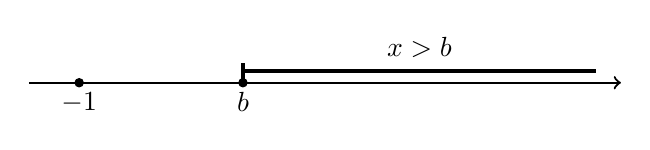
\begin{tikzpicture}[x=1.6cm,y=1cm]
			\draw[thick,->] (-0.5,0) -- (4.2,0);
			
			\filldraw (-0.1,0) circle (1.5pt);
			\node[below] at (-0.1,0) {$-1$};
			
			\filldraw (1.2,0) circle (1.5pt);
			\node[below] at (1.2,0) {$b$};
			
			\draw[very thick] (1.2,0.15) -- (4,0.15);
			\draw[very thick] (1.2,0.05) -- (1.2,0.25);
			
			\node[above] at (2.6,0.2) {$x>b$};
		\end{tikzpicture}
	\end{center}
	
	Para que la inecuación sea lineal, el coeficiente de $x^2$ debe ser cero:
	
	$a+1=0 \Rightarrow a=-1$
	
	Entonces la inecuación queda:
	
	$-x+b<0$
	
	De aquí:
	
	$x>b$
	
	Además, como $a<b$ y $a=-1$, se tiene:
	
	$-1<b$
	
	Por tanto:
	
	$x>b>-1$
	
	Luego, el conjunto solución es de la forma:
	
	$\langle,+\infty\rangle \subset \langle -1,+\infty\rangle$
	
	\fbox{$\langle -1;+\infty\rangle$}
	
	\vspace{6mm}
	
	\item La función $T(t)=T_m+(T_0-T_m)e^{-kt}$ representa la ley de enfriamiento de un cuerpo, donde $T(t)$ es la temperatura del cuerpo después de un tiempo $t$ dado en minutos, $T_0$ y $T_m$ representan la temperatura inicial del cuerpo y la temperatura del medio respectivamente. Según esta ley: si una taza de leche se enfría de $90^\circ C$ a $60^\circ C$ en 10 minutos en la habitación donde la temperatura es de $30^\circ C$, halle el valor de la constante $k$.
	\begin{enumerate}[label=\alph*)]
		\item $-\dfrac{\ln 2}{10}$
		\item $\dfrac{10}{\ln 2}$
		\item $-\dfrac{\ln 3}{10}$
		\item $\dfrac{\ln 2}{10}$
		\item $\dfrac{10}{\ln 3}$
	\end{enumerate}
	\textbf{Respuesta correcta:} d)
	
	\vspace{2mm}
	\textbf{Solucionario:}\\[1mm]
	Sustituyendo en la ley de enfriamiento:
	
	$60=30+(90-30)e^{-10k}$
	
	$60=30+60e^{-10k}$
	
	$\dfrac{30}{60}=e^{-10k}$
	
	$\dfrac{1}{2}=e^{-10k}$
	
	
	$\ln\left(\dfrac{1}{2}\right)=-10k$
	
	$-\ln 2=-10k$
	
	$k=\dfrac{\ln 2}{10}$
	
	\fbox{$k=\dfrac{\ln 2}{10}$}
	
	\vspace{6mm}
	
	\item El cociente notable $\dfrac{x^n-y^m}{x^3-y^4}$ tiene 14 términos en su desarrollo. El grado absoluto del séptimo término del desarrollo representa la edad de Adrián dentro de 3 años. Halle $m+n$ menos la edad de Adrián.
	\begin{enumerate}[label=\alph*)]
		\item 42
		\item 56
		\item 45
		\item 48
		\item 98
	\end{enumerate}
	\textbf{Respuesta correcta:} b)
	
	\vspace{2mm}
	\textbf{Solucionario:}\\[1mm]
	Como el cociente notable tiene $14$ términos, se cumple:
	
	$\dfrac{n}{3}=\dfrac{m}{4}=14$
	
	De donde:
	
	$n=42,\qquad m=56$
	
	El séptimo término del desarrollo es:
	
	$t_7=(x^3)^{14-7}(y^4)^{7-1}=x^{21}y^{24}$
	
	
	$GA(t_7)=21+24=45$
	
	Como ese valor representa la edad de Adrián dentro de $3$ años, su edad actual es:
	
	$45-3=42$
	
	Por tanto:
	
	\fbox{$m+n-42=56$}
	
	\vspace{6mm}
	
\end{enumerate}

\subsection*{Geometría}

\begin{enumerate}[resume]
	
	\item Jonás tiene una madera de forma triangular, pero solo necesita una parte. Por ello, traza $BM$ por donde realizará el corte. Si $AB=80$ cm, $BC=1$ m y $M$ es punto medio de $AC$, halle la longitud de corte.
	\begin{center}
 		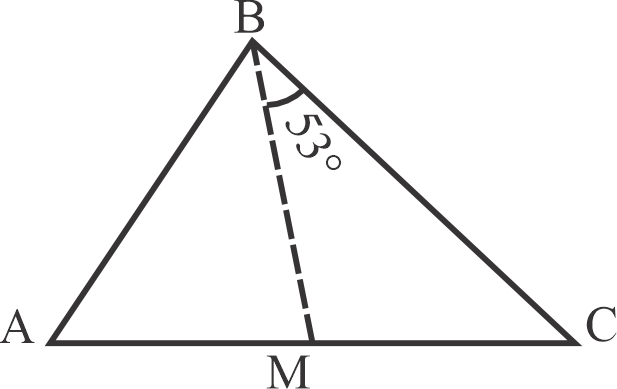
\includegraphics[width=4.4cm]{imagenes/CEPRE-UNA2024-I/etapa2/bio/geo1c24-I.png}
	\end{center}
	\begin{enumerate}[label=\alph*)]
		\item 30 cm
		\item 45 cm
		\item 50 cm
		\item 40 cm
		\item 35 cm
	\end{enumerate}
	\textbf{Respuesta correcta:} a)
	
	\vspace{2mm}
	\textbf{Solucionario:}
	
	\begin{center}
		\begin{minipage}{0.45\textwidth}
			
		Piden $BM=x$
		
		Trazamos $MN$ base media del triángulo ABC.

		Como $N$ es punto medio  de $BC$ y $HC=2MN$, se tiene que $MN$ también es base media del triángulo rectángulo $BHC$.
		
		Entonces, el triángulo $BHC$ es notable de $37^\circ$ y $53^\circ$, por lo que sus lados están en razón:
		
		$3k,\ 4k,\ 5k$
		
		Del gráfico se obtiene:
		
		$2x=60$
		
		Por tanto:
		
		$x=30\text{ cm}$
		
		\fbox{$30\text{ cm}$}
			\vspace{6mm}
		\end{minipage}
		\hfill
		\begin{minipage}{0.45\textwidth}
			\centering
			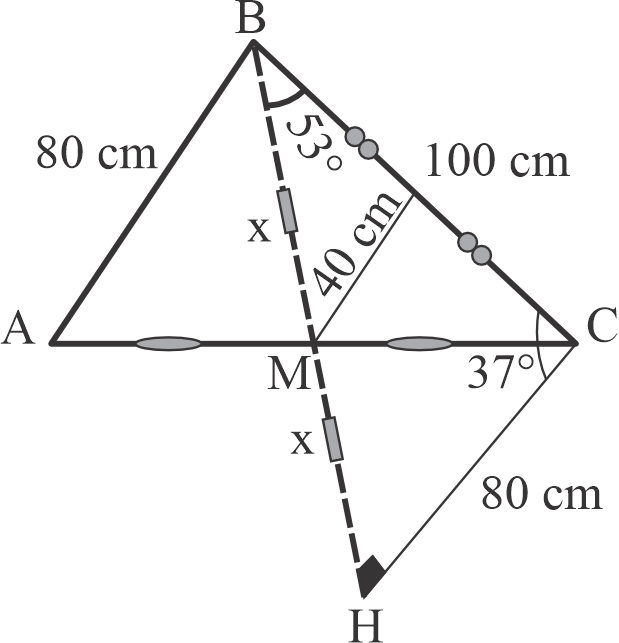
\includegraphics[width=4cm]{imagenes/CEPRE-UNA2024-I/etapa2/bio/geo1c24-Ir.png}
		\end{minipage}
		\end{center}
	
	\vspace{6mm}
	
	\item Se tiene un hexágono equiángulo $ABCDEF$ de tal manera que $AB=3$, $BC=6$, $EF=2$ y $AF=9$. Calcule las longitudes de $\overline{CD}$ y $\overline{DE}$.
	\begin{enumerate}[label=\alph*)]
		\item 4 y 7
		\item 5 y 7
		\item 7 y 6
		\item 7 y 3
		\item 4 y 5
	\end{enumerate}
	\textbf{Respuesta correcta:} b)
	
	\vspace{2mm}
	\textbf{Solucionario:}\\[1mm]
	
	
		\begin{center}
		\begin{minipage}{0.45\textwidth}
			
	
			Como el polígono es equiángulo, cada ángulo exterior mide:
			
			$\dfrac{360^\circ}{6}=60^\circ$
			
			Al prolongar los lados, se forman triángulos equiláteros auxiliares.
			
			De la figura se obtiene que:
			
			$PR=14$
			\qquad y \qquad
			$PQ=14$
			
			Entonces:
			
			$3+6+x=14$
			
			$9+x=14$
			
			$x=5$
			
			Además:
			
			$x+y+2=14$
			
			$5+y+2=14$
			
			$y=7$
			
			Por lo tanto:
			
			$CD=x=5,\qquad DE=y=7$
			
			\fbox{$CD=5,\ DE=7$}
			\vspace{6mm}
		\end{minipage}
		\hfill
		\begin{minipage}{0.45\textwidth}
			\centering
			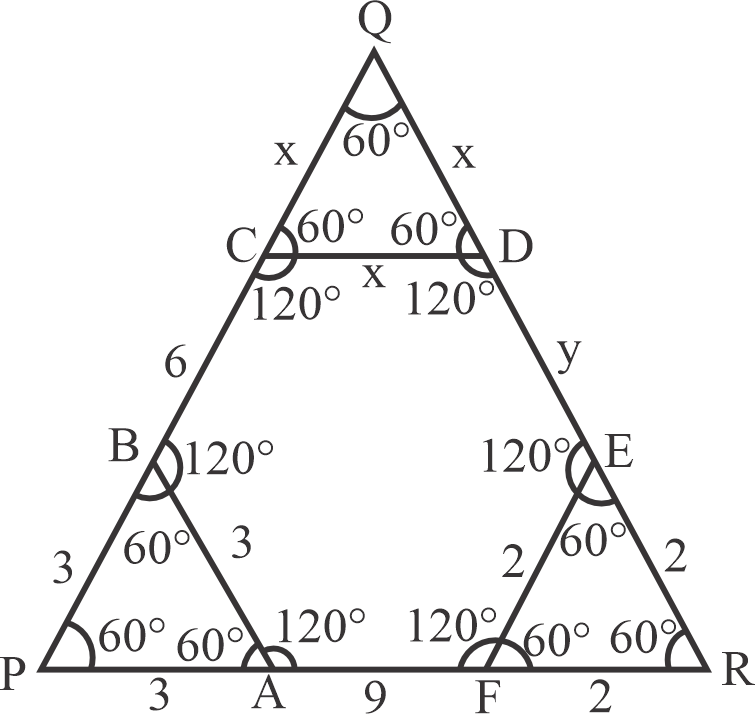
\includegraphics[width=4.2cm]{imagenes/CEPRE-UNA2024-I/etapa2/bio/geo2c24-Ir.png}
		\end{minipage}
	\end{center}
	

	
	\vspace{6mm}
	
	\item Marcos construye una mesa cuyo tablero tiene la forma de un trapecio isósceles, tal como se muestra en el gráfico. Calcule el perímetro del tablero de la mesa.
	\begin{center}
		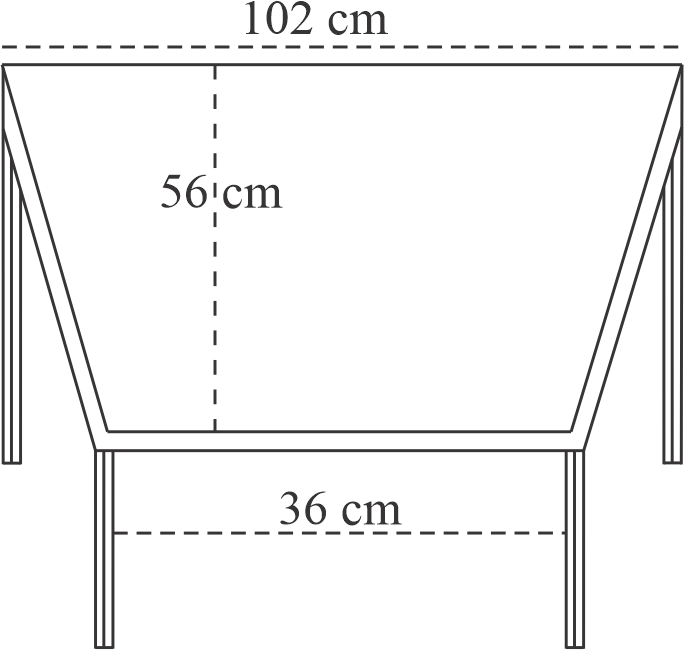
\includegraphics[width=4.3cm]{imagenes/CEPRE-UNA2024-I/etapa2/bio/geo3c24-I.png}
	\end{center}
	
	\begin{enumerate}[label=\alph*)]
		\item 230 cm
		\item 258 cm
		\item 260 cm
		\item 268 cm
		\item 278 cm
	\end{enumerate}
	\textbf{Respuesta correcta:} d)
	
	\vspace{2mm}
	\textbf{Solucionario:}

			\begin{center}
		\begin{minipage}{0.45\textwidth}
			
			
		Bases:

		$B=102,\qquad b=36,\qquad h=56$
		
		La semidiferencia de bases es:\\
		
		$\dfrac{102-36}{2}=33$\\
		
		Cada lado oblicuo mide:\\
		
		$l=\sqrt{33^2+56^2}=\sqrt{1089+3136}=\sqrt{4225}=65$
		
		Entonces el perímetro es:
		
		$P=102+36+65+65=$\fbox{$268$}
			\vspace{6mm}
		\end{minipage}
		\hfill
		\begin{minipage}{0.45\textwidth}
			\centering
			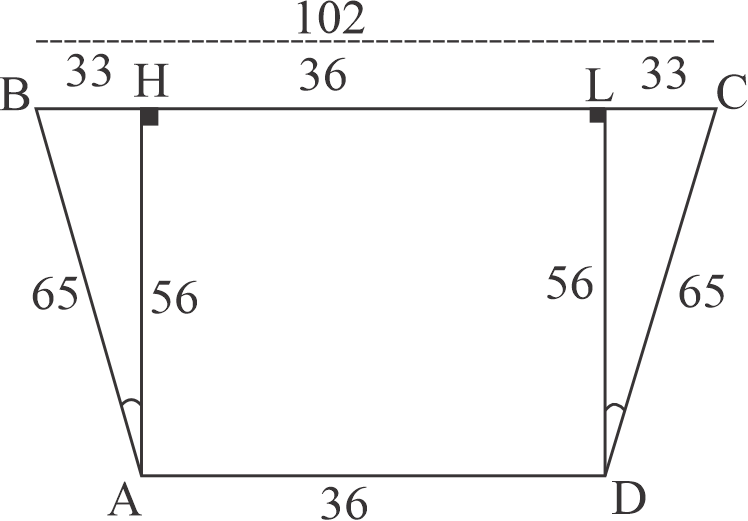
\includegraphics[width=4.5cm]{imagenes/CEPRE-UNA2024-I/etapa2/bio/geo3c24-Ir.png}
		\end{minipage}
	\end{center}
	
	\vspace{6mm}
	
\end{enumerate}

\subsection*{Trigonometría}

\begin{enumerate}[resume]

	
	\item En la figura, calcule el área de la región sombreada si $OA=OB$ y $AC=BD$.
	
	\begin{center}
		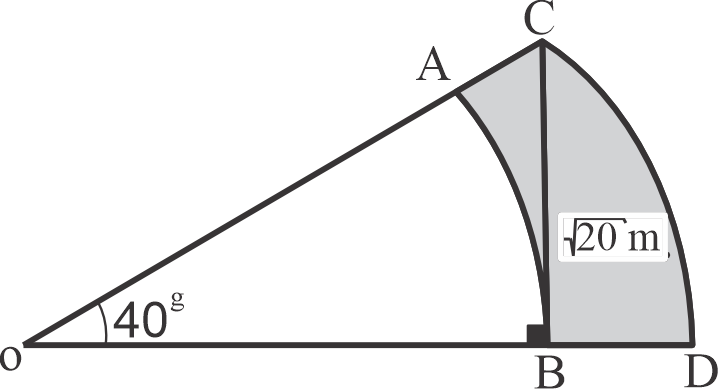
\includegraphics[width=4.3cm]{imagenes/CEPRE-UNA2024-I/etapa2/bio/trigo1c24-I.png}
	\end{center}
	
	\begin{enumerate}[label=\alph*)]
		\item $\pi\ m^2$
		\item $2\pi\ m^2$
		\item $3\pi\ m^2$
		\item $4\pi\ m^2$
		\item $5\pi\ m^2$
	\end{enumerate}
	\textbf{Respuesta correcta:} b)
	
	\vspace{2mm}
	\textbf{Solucionario:}\\[1mm]
	Como $40^g=\dfrac{40\pi}{200}=\dfrac{\pi}{5}\text{ rad}$
	
	$\theta=\dfrac{\pi}{5}$
	
	Además, en el triángulo rectángulo formado por los radios y la distancia entre circunferencias:
	
	$R^2=r^2+(\sqrt{20})^2$
	
	$R^2-r^2=20$
	
	El área sombreada es la diferencia de dos sectores:
	
	$A_{\text{sombreada}}=\dfrac{\theta R^2}{2}-\dfrac{\theta r^2}{2}$
	
	$=\dfrac{\theta}{2}(R^2-r^2)$
	
	$=\dfrac{1}{2}\cdot \dfrac{\pi}{5}\cdot 20$
	
	$=2\pi \text{ m}^2$
	
	\fbox{$2\pi \text{ m}^2$}
	
	
	\vspace{6mm}
	
	\item En la figura, si $AB=12\sqrt{3}$ y $BC=4\sqrt{3}$, calcule $AD+CD$.
	
	\begin{center}
		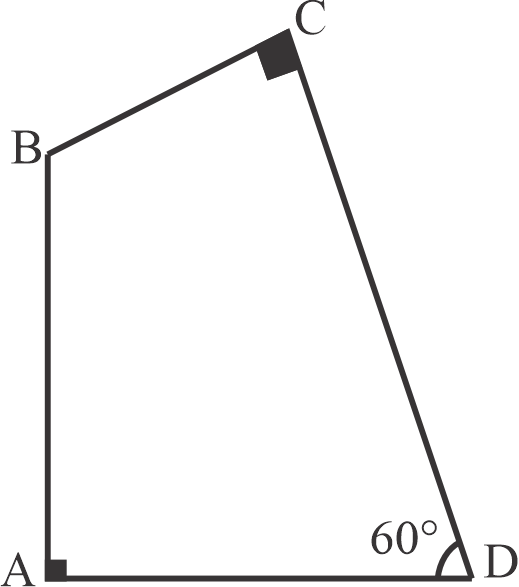
\includegraphics[width=3.8cm]{imagenes/CEPRE-UNA2024-I/etapa2/bio/trigo2c24-I.png}
	\end{center}
	
	\begin{enumerate}[label=\alph*)]
		\item 40
		\item 46
		\item 38
		\item 50
		\item 48
	\end{enumerate}
	\textbf{Respuesta correcta:} e)
	
	\vspace{2mm}
	\textbf{Solucionario:}

	En el gráfico inicial se continua con el trazo de $AB$ y $DC$ hacia el punto $A$, se reconoce que los triángulos $ADE$ y $BCE$ son triángulos notables de $30^\circ$ y $60^\circ$.
	
	Por ello, los segmentos correspondientes resultan:
	
	$AD=20$
	\qquad y \qquad
	$DC=28$
	
	Entonces:
	
	$AD+DC=20+28=$\fbox{$48$}
	
	\vspace{6mm}
	

	\item Si $3\sen x+4\cos x=5$, calcule $\tan x+\dfrac{5}{4}$.
	\begin{enumerate}[label=\alph*)]
		\item 1
		\item 0
		\item 2
		\item $\dfrac{1}{4}$
		\item $\dfrac{3}{4}$
	\end{enumerate}
	\textbf{Respuesta correcta:} c)
	
	\vspace{2mm}
	\textbf{Solucionario:}\\[1mm]
	
	\begin{center}
		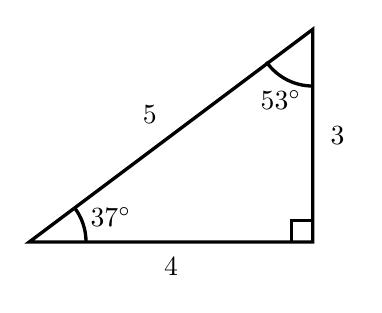
\begin{tikzpicture}[scale=0.9]
			\draw[very thick] (0,0) -- (4,0) -- (4,3) -- cycle;
			\draw[very thick] (3.7,0) -- (3.7,0.3) -- (4,0.3);
			\node at (2, -0.35) {$4$};
			\node at (4.35,1.5) {$3$};
			\node at (1.7,1.8) {$5$};
			\draw[very thick] (0.8,0) arc[start angle=0,end angle=37,radius=0.8];
			\node at (1.15,0.35) {$37^\circ$};
			\draw[very thick] (4,2.2) arc[start angle=270,end angle=215,radius=0.8];
			\node at (3.55,2) {$53^\circ$};
		\end{tikzpicture}
	\end{center}
	
	Dividimos entre $5$:
	
	$\dfrac{3}{5}\sen x+\dfrac{4}{5}\cos x=1$
	
	Como $\dfrac{3}{5}$ y $\dfrac{4}{5}$ corresponden a un triángulo notable $3$-$4$-$5$, tomamos:
	
	$\cos 53^\circ=\dfrac{3}{5}, \qquad \sen 53^\circ=\dfrac{4}{5}$
	
	Entonces:
	
	$\cos 53^\circ \sen x+\sen 53^\circ \cos x=1$
	
	
	$\sen(x+53^\circ)=1$
	
	
	$x+53^\circ=90^\circ$
	
	$x=37^\circ$
	
	
	$\tan x+\dfrac{5}{4}=\tan 37^\circ+\dfrac{5}{4}$
	
	$=\dfrac{3}{4}+\dfrac{5}{4}=$\fbox{$2$}
	
	\vspace{6mm}
	
\end{enumerate}

\subsection*{Física}

\begin{enumerate}[resume]
	
	
	\item En la figura, calcule el valor de la fuerza $\vec{F}$ para que el cuerpo de 40 N de peso permanezca en equilibrio.
	
	\begin{center}
		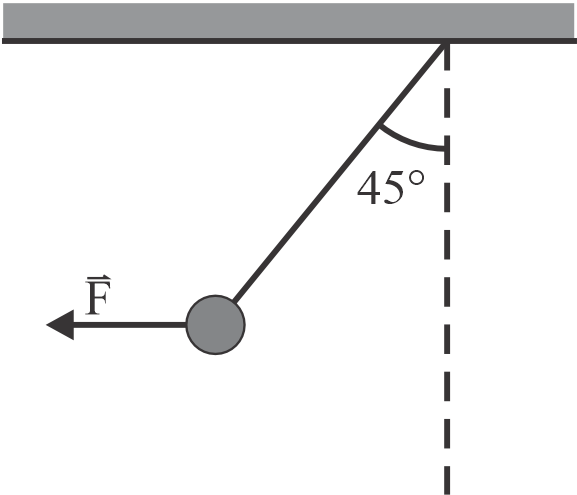
\includegraphics[width=4cm]{imagenes/CEPRE-UNA2024-I/etapa2/bio/fisica1c24-I.png}
	\end{center}
	
	\begin{enumerate}[label=\alph*)]
		\item 20 N
		\item $20\sqrt{2}$ N
		\item 40 N
		\item $40\sqrt{2}$ N
		\item 45 N
	\end{enumerate}
	\textbf{Respuesta correcta:} c)
	
	\vspace{2mm}
	\textbf{Solucionario:}\\[1mm]
	La tensión forma $45^\circ$ con la vertical. En equilibrio:
	
	$T\cos45^\circ=40$
	
	$T=\dfrac{40}{\cos45^\circ}=40\sqrt2$
	
	La fuerza horizontal es:
	
	$F=T\sen45^\circ=40\sqrt2\cdot \dfrac{\sqrt2}{2}=$\fbox{$40N$}
	
	\vspace{6mm}
	

	
	\item Desde la superficie terrestre se lanza un proyectil con una velocidad de 50 m/s formando un ángulo de $53^\circ$ con la horizontal. Determine el valor de la velocidad del proyectil en el punto más alto de su trayectoria.
	\begin{enumerate}[label=\alph*)]
		\item 20 m/s
		\item 30 m/s
		\item 40 m/s
		\item 50 m/s
		\item 60 m/s
	\end{enumerate}
	\textbf{Respuesta correcta:} b)
	
	\vspace{2mm}
	\textbf{Solucionario:}\\[1mm]
	En el punto más alto, la componente vertical es cero y solo queda la horizontal:
	
	$v_x=50\cos53^\circ$
	
	Usando:
	
	$\cos53^\circ=\dfrac35$
	
	se obtiene:
	
	$v_x=50\cdot \dfrac{3}{5}=$\fbox{$30N$}
	
	\vspace{6mm}
	
	
	\item Una máquina soldadora de 1000 W funciona a un voltaje de 220 V. Determine la energía eléctrica que consume en 20 minutos de funcionamiento.
	\begin{enumerate}[label=\alph*)]
		\item 0,6 MJ
		\item 1,0 MJ
		\item 1,2 MJ
		\item 2,2 MJ
		\item 4,4 MJ
	\end{enumerate}
	\textbf{Respuesta correcta:} c)
	
	\vspace{2mm}
	\textbf{Solucionario:}\\[1mm]
	La energía es:
	
	$E=Pt$
	
	Con:
	
	$P=1000\text{ W},\qquad t=20\text{ min}=1200\text{ s}$
	
	Entonces:
	
	$E=1000(1200)=1\,200\,000\text{ J}=$\fbox{$1.2\text{ MJ}$}
	
	\vspace{6mm}
	
\end{enumerate}

  \subsection*{Química}

\begin{enumerate}[resume]
	
	\item Se tiene dos isótopos los cuales tienen 20 y 24 neutrones respectivamente. Si la suma de sus números de nucleones fundamentales es 104, determine la ubicación de dicho elemento en la tabla periódica.
	\begin{enumerate}[label=\alph*)]
		\item período 3: grupo 4B
		\item período 4: grupo 2B
		\item período 4: grupo 6B
		\item período 4: grupo 3B
		\item período 5: grupo 1B
	\end{enumerate}
	\textbf{Respuesta correcta:} b)
	
	\vspace{2mm}
	\textbf{Solucionario:}\\[1mm]
	Sea $Z$ el número atómico. Los números másicos son:
	
	$A_1=Z+20,\qquad A_2=Z+24$
	
	Su suma es 104:
	
	$(Z+20)+(Z+24)=104$
	
	$2Z+44=104$
	
	$2Z=60 \Rightarrow Z=30$
	
	El elemento con $Z=30$ es Zn, ubicado en período 4, grupo 2B.
	
	\vspace{6mm}
	
	\item Después del balanceo en medio ácido de la ecuación iónica:
	
	$\mathrm{Fe^{2+}_{(ac)}+ClO_3^-{}_{(ac)}\rightarrow Fe^{3+}_{(ac)}+Cl^-{}_{(ac)}}$
	
	indique el coeficiente del agua.
	\begin{enumerate}[label=\alph*)]
		\item 2
		\item 3
		\item 4
		\item 5
		\item 6
	\end{enumerate}
	\textbf{Respuesta correcta:} b)
	
	\vspace{2mm}
	\textbf{Solucionario:}\\[1mm]
	Semirreacciones:
	
	$Fe^{2+}\rightarrow Fe^{3+}+e^-$
	
	$ClO_3^-+6H^++6e^-\rightarrow Cl^-+3H_2O$
	
	Multiplicando la primera por 6 y sumando:
	
	$6Fe^{2+}+ClO_3^-+6H^+\rightarrow 6Fe^{3+}+Cl^-+3H_2O$
	
	El coeficiente del agua es \fbox{3}
	
	\vspace{6mm}
	
	\item Un balón contiene metano ($CH_4$) a $30^\circ C$ y 0,4 atm. Calcule la presión que tendrá si aumentamos la temperatura hasta $200^\circ C$ permaneciendo su volumen constante.
	\begin{enumerate}[label=\alph*)]
		\item 0,26 atm
		\item 0,29 atm
		\item 0,31 atm
		\item 0,38 atm
		\item 0,62 atm
	\end{enumerate}
	\textbf{Respuesta correcta:} e)
	
	\vspace{2mm}
	\textbf{Solucionario:}\\[1mm]
	A volumen constante:
	
	$\dfrac{P_1}{T_1}=\dfrac{P_2}{T_2}$
	
	Temperaturas absolutas:
	
	$T_1=30+273=303,\qquad T_2=200+273=473$
	
	Entonces:
	
	$P_2=0.4\cdot \dfrac{473}{303}\approx \fbox{0.62}$
	
	\vspace{6mm}
	
	\item Proporcione el nombre IUPAC del alcano cuya notación topológica es:
	
	\begin{center}
		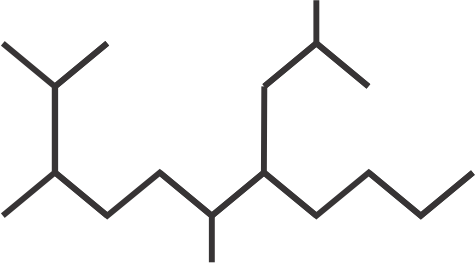
\includegraphics[width=4.5cm]{imagenes/CEPRE-UNA2024-I/etapa2/bio/quimica4c24-I.png}
	\end{center}
	
	\begin{enumerate}[label=\alph*)]
		\item 7-isobutil-2,3,6-trimetilundecano
		\item 5-isobutil-6,9,19-trimetilundecano
		\item 3-sec-butil-5,3,4-dimetilundecano
		\item 5-etil-5,6,11-trimetil-4-terbutilnonano
		\item 7-butil-2,3,6,9-tetrametildecano
	\end{enumerate}
	\textbf{Respuesta correcta:} a)
	
	\vspace{2mm}
	\textbf{Solucionario:}\\[1mm]
	Se identifica como cadena principal una de 11 carbonos, es decir, un undecano. Al numerar para obtener el menor conjunto de localizadores, se observan tres metilos en 2, 3 y 6, y un isobutil en 7. Por ello, el nombre correcto es:
	
	$\text{7-isobutil-2,3,6-trimetilundecano}$
	
	\vspace{6mm}
	
	\item El grupo de vitaminas B es muy complejo. Tenemos por ejemplo la vitamina $B_1$ cuya fórmula es $C_{12}H_{17}N_4OS$ y la vitamina $B_2$ cuya fórmula es $C_{17}H_{20}N_4O_6$. Entonces la suma de sus pesos moleculares es:
	\begin{enumerate}[label=\alph*)]
		\item 700
		\item 641
		\item 376
		\item 265
		\item 670
	\end{enumerate}
	\textbf{Respuesta correcta:} b)
	
	\vspace{2mm}
	\textbf{Solucionario:}\\[1mm]
	Usando masas atómicas: $C=12$, $H=1$, $N=14$, $O=16$, $S=32$.
	
	Para $B_1$:
	
	$12(12)+17(1)+4(14)+16+32=265$
	
	Para $B_2$:
	
	$17(12)+20(1)+4(14)+6(16)=376$
	
	Suma:
	
	\fbox{$265+376=641$}
	
	\vspace{6mm}
	
\end{enumerate}

\subsection*{Biología y Anatomía}

\begin{enumerate}[resume]
	
	\item Juan desarrolla anemia si su cuerpo no produce suficientes glóbulos rojos. ¿Cuál es el bioelemento insuficiente que presenta?
	\begin{enumerate}[label=\alph*)]
		\item Insulina
		\item Hierro
		\item Glucagón
		\item Iodo
		\item Glucosa
	\end{enumerate}
	\textbf{Respuesta correcta:} b)
	
	\vspace{2mm}
	\textbf{Solucionario:}\\[1mm]
	La anemia suele asociarse a la deficiencia de hierro, porque este elemento es esencial para la formación de hemoglobina y glóbulos rojos.
	
	\vspace{6mm}
	
	\item Los animales que pueden variar su temperatura corporal modificando su comportamiento en estrecha relación a la temperatura ambiental se denominan:
	\begin{enumerate}[label=\alph*)]
		\item homeotermos.
		\item poiquilotermos.
		\item endotermos.
		\item homotermos.
		\item depredadores.
	\end{enumerate}
	\textbf{Respuesta correcta:} b)
	
	\vspace{2mm}
	\textbf{Solucionario:}\\[1mm]
	Los poiquilotermos son organismos cuya temperatura corporal varía de acuerdo con la temperatura del ambiente.
	
	\vspace{6mm}
	
	\item Algunas serpientes incuban sus huevos en el interior del oviducto donde eclosionan liberando sus crías. Este tipo de nacimiento corresponde a:
	\begin{enumerate}[label=\alph*)]
		\item ovíparos.
		\item ovovivíparos.
		\item metamorfosis.
		\item vivíparos.
		\item fragmentación.
	\end{enumerate}
	\textbf{Respuesta correcta:} b)
	
	\vspace{2mm}
	\textbf{Solucionario:}\\[1mm]
	En los ovovivíparos, los huevos permanecen dentro del cuerpo de la madre hasta su eclosión, pero el embrión se nutre del huevo, no directamente de la madre.
	
	\vspace{6mm}
	
	\item Las haustras, tenias musculares y apéndices cecales son estructuras que corresponden al:
	\begin{enumerate}[label=\alph*)]
		\item estómago.
		\item intestino delgado.
		\item esófago.
		\item hígado.
		\item intestino grueso.
	\end{enumerate}
	\textbf{Respuesta correcta:} e)
	
	\vspace{2mm}
	\textbf{Solucionario:}\\[1mm]
	Las haustras, tenias del colon y apéndices epiploicos son características anatómicas del intestino grueso.
	
	\vspace{6mm}
	
	\item En el ciclo del nitrógeno, intervienen bacterias nitrificantes y bacterias fijadoras de nitrógeno. Ejemplos de ellas son:
	\begin{enumerate}[label=\alph*)]
		\item nitrosomonas -- rhizobium.
		\item nitrosomonas -- nitrobacter.
		\item rhizobium -- azotobacter.
		\item nitrobacter -- nitrosomonas.
		\item azotobacter -- rhizobium.
	\end{enumerate}
	\textbf{Respuesta correcta:} a)
	
	\vspace{2mm}
	\textbf{Solucionario:}\\[1mm]
	\textit{Nitrosomonas} es bacteria nitrificante y \textit{Rhizobium} es fijadora de nitrógeno. La pareja correcta es:
	
	$\text{nitrosomonas -- rhizobium}$
	
	\vspace{6mm}
	
	\item El principal efecto de los compuestos fluorocarbonados utilizados como refrigerantes es que al ser liberados a la atmósfera:
	\begin{enumerate}[label=\alph*)]
		\item producen acumulación en tejidos orgánicos.
		\item provocan efecto smog fotoquímico.
		\item provocan la lluvia ácida.
		\item destruyen la capa de ozono.
		\item producen la eutroficación.
	\end{enumerate}
	\textbf{Respuesta correcta:} d)
	
	\vspace{2mm}
	\textbf{Solucionario:}\\[1mm]
	Los clorofluorocarbonos y compuestos similares afectan la capa de ozono estratosférica, favoreciendo su destrucción.
	
	\vspace{6mm}
	
\end{enumerate}

\subsection*{Psicología y Filosofía}

\begin{enumerate}[resume]
	
	\item El principio y el fin de todo conocimiento es la:
	\begin{enumerate}[label=\alph*)]
		\item teoría.
		\item especulación.
		\item ciencia.
		\item práctica.
		\item argumentación.
	\end{enumerate}
	\textbf{Respuesta correcta:} d)
	
	\vspace{2mm}
	\textbf{Solucionario:}\\[1mm]
	En filosofía se sostiene que la práctica es la base y comprobación del conocimiento, por lo que se considera el principio y fin del mismo.
	
	\vspace{6mm}
	
	\item Cuando la persona moral se da cuenta que los actos que realiza son buenos o malos, estamos haciendo referencia a:
	\begin{enumerate}[label=\alph*)]
		\item libertad moral.
		\item acto moral.
		\item conciencia moral.
		\item responsabilidad moral.
		\item libertad de conciencia.
	\end{enumerate}
	\textbf{Respuesta correcta:} c)
	
	\vspace{2mm}
	\textbf{Solucionario:}\\[1mm]
	La conciencia moral es la capacidad de juzgar los propios actos como buenos o malos.
	
	\vspace{6mm}
	
	\item La disciplina filosófica que se encarga de estudiar la ciencia y la estructura del conocimiento es la:
	\begin{enumerate}[label=\alph*)]
		\item axiología.
		\item epistemología.
		\item traumatología.
		\item sociología.
		\item fenomenología.
	\end{enumerate}
	\textbf{Respuesta correcta:} b)
	
	\vspace{2mm}
	\textbf{Solucionario:}\\[1mm]
	La epistemología estudia la naturaleza, origen y validez del conocimiento científico.
	
	\vspace{6mm}
	
	\item Es el cambio más complejo que incluye transformaciones en el funcionamiento y desarrollo de la inteligencia, creatividad, sociabilidad y moralidad.
	\begin{enumerate}[label=\alph*)]
		\item Cambio cualitativo
		\item Cambio cuantitativo
		\item Metamorfosis
		\item Cambio dimensional
		\item Maduración
	\end{enumerate}
	\textbf{Respuesta correcta:} a)
	
	\vspace{2mm}
	\textbf{Solucionario:}\\[1mm]
	El cambio cualitativo implica modificaciones profundas en la manera de pensar, actuar y desarrollarse, no solo aumento en cantidad. Por ello se relaciona con inteligencia, creatividad, sociabilidad y moralidad.
	
	\vspace{6mm}
	
\end{enumerate}

\subsection*{Geografía}

\begin{enumerate}[resume]
	
	\item La unidad minera que explota yacimientos de cobre en el departamento de Apurímac es:
	\begin{enumerate}[label=\alph*)]
		\item Antamina.
		\item Las Bambas.
		\item Cobriza.
		\item Tintaya.
		\item Cerro Verde.
	\end{enumerate}
	\textbf{Respuesta correcta:} b)
	
	\vspace{2mm}
	\textbf{Solucionario:}\\[1mm]
	Las Bambas es el importante proyecto cuprífero ubicado en la región Apurímac.
	
	\vspace{6mm}
	
	\item El mar peruano es considerado uno de los más ricos y variados a nivel mundial debido a la:
	\begin{enumerate}[label=\alph*)]
		\item ubicación geográfica del Perú.
		\item cercanía de la Cordillera de los Andes.
		\item presencia de nubes stratos.
		\item descarga constante de sedimentos de ríos.
		\item abundancia de fitoplancton.
	\end{enumerate}
	\textbf{Respuesta correcta:} e)
	
	\vspace{2mm}
	\textbf{Solucionario:}\\[1mm]
	La riqueza del mar peruano se debe, entre otros factores, a la abundancia de fitoplancton, base de la cadena alimenticia marina.
	
	\vspace{6mm}
	
\end{enumerate}

\subsection*{Historia}

\begin{enumerate}[resume]
	
	\item Fue el impuesto que gravaba los cargos públicos, lo que debían pagar aquellos que asumían un cargo administrativo antes de ejercer el mismo.
	\begin{enumerate}[label=\alph*)]
		\item Derecho de avería
		\item El almojarifazgo
		\item El tributo indígena
		\item La alcabala
		\item La media anata
	\end{enumerate}
	\textbf{Respuesta correcta:} e)
	
	\vspace{2mm}
	\textbf{Solucionario:}\\[1mm]
	La media anata era el tributo que debían pagar quienes accedían a determinados cargos públicos.
	
	\vspace{6mm}
	
	\item Es el presidente que, en 1933, pasaba revista a los 30 mil movilizables en el antiguo Hipódromo de Santa Beatriz, hoy Campo de Marte en Lima, y fue asesinado por Abelardo Mendoza Leyva de tres tiros de revólver.
	\begin{enumerate}[label=\alph*)]
		\item Oscar Raymundo Benavides
		\item Manuel Prado Ugarteche
		\item José Luis Bustamante y Rivero
		\item Luís Miguel Sánchez Cerro
		\item Augusto Bernardino Leguía
	\end{enumerate}
	\textbf{Respuesta correcta:} d)
	
	\vspace{2mm}
	\textbf{Solucionario:}\\[1mm]
	El presidente asesinado en 1933 fue Luis Miguel Sánchez Cerro.
	
	\vspace{6mm}
	
\end{enumerate}

\subsection*{Educación Cívica}

\begin{enumerate}[resume]
	
	\item Marcos está casado con Juana por un período de 5 años; sin embargo, Juana toma conocimiento que Marcos tiene un hijo extramatrimonial de 1 año, hecho que corrobora con el acta de nacimiento. ¿Qué causal podría invocar Juana para que declaren fundada su demanda de divorcio?
	\begin{enumerate}[label=\alph*)]
		\item Servicia
		\item Hijo extramatrimonial
		\item Engaño
		\item Adulterio
		\item Infidelidad
	\end{enumerate}
	\textbf{Respuesta correcta:} d)
	
	\vspace{2mm}
	\textbf{Solucionario:}\\[1mm]
	El hijo de 1 año prueba que Marcos tuvo relaciones con otra mujer durante el matrimonio, lo que constituye adulterio.
	
	\vspace{6mm}
	
	\item En el año 2019, entró en vigencia la ley de plásticos como respuesta del país ante la grave situación que enfrentan los mares del mundo por la contaminación. En el corto plazo, los supermercados fueron prohibidos de entregar bolsas de plástico no reutilizables, fabricar sorbetes para el consumo interno, entre otras medidas importantes. Todo lo anterior está vinculado con la preservación del medio ambiente sano que es clasificado como un derecho humano de:
	\begin{enumerate}[label=\alph*)]
		\item primera generación.
		\item segunda generación.
		\item tercera generación.
		\item cuarta generación.
		\item pre generación.
	\end{enumerate}
	\textbf{Respuesta correcta:} c)
	
	\vspace{2mm}
	\textbf{Solucionario:}\\[1mm]
	Los derechos relacionados con el ambiente sano, la paz y el desarrollo pertenecen a la tercera generación de derechos humanos.
	
	\vspace{6mm}
	
\end{enumerate}

\subsection*{Economía}

\begin{enumerate}[resume]
	
	\item La estructura del presupuesto público en el Perú comprende los gastos corrientes que:
	\begin{enumerate}[label=\alph*)]
		\item incluye el pago de salarios del personal que labora en el sector público.
		\item son destinados a proyectos de inversión a largo plazo.
		\item son relacionados con la deuda externa del país.
		\item son categorías separadas en el presupuesto y no están vinculadas a actividades diarias.
		\item incluye los otros gastos de capital.
	\end{enumerate}
	\textbf{Respuesta correcta:} a)
	
	\vspace{2mm}
	\textbf{Solucionario:}\\[1mm]
	Los gastos corrientes financian el funcionamiento ordinario del Estado, como remuneraciones, bienes y servicios.
	
	\vspace{6mm}
	
	\item Es el proceso de acumulación progresiva durante un período más o menos prolongado de una parte de los ingresos percibidos.
	\begin{enumerate}[label=\alph*)]
		\item El ingreso
		\item La producción
		\item La inversión
		\item El capital
		\item El ahorro
	\end{enumerate}
	\textbf{Respuesta correcta:} e)
	
	\vspace{2mm}
	\textbf{Solucionario:}\\[1mm]
	El ahorro consiste en reservar o acumular una parte del ingreso para uso futuro.
	
	\vspace{6mm}
	
\end{enumerate}

\subsection*{Comunicación}

\begin{enumerate}[resume]
	
	\item En una conversación, un botánico afirma: “Las plantas del patio crecen al recibir luz solar y agua. Las plantas del vecino crecen al recibir luz solar y agua. Las plantas del jardín botánico crecen al recibir luz solar y agua. Entonces las plantas crecen al recibir la luz solar y el agua”.
	
	Considerando la redacción, las ideas están expresadas en forma:
	\begin{enumerate}[label=\alph*)]
		\item deductiva.
		\item inductiva.
		\item mixta.
		\item paremiológica.
		\item compleja.
	\end{enumerate}
	\textbf{Respuesta correcta:} b)
	
	\vspace{2mm}
	\textbf{Solucionario:}\\[1mm]
	Se presentan varios casos particulares y luego una conclusión general. Eso corresponde a razonamiento inductivo.
	
	\vspace{6mm}
	
	\item Cuando la Constitución Política del Perú declara como idiomas oficiales al quechua, aimara y lenguas originarias amazónicas quiere decir que:
	\begin{enumerate}[label=\alph*)]
		\item no se deben usar en público.
		\item se obliga su uso a todos los ciudadanos.
		\item están facultados para uso público e institucional.
		\item se reconocen como un derecho humano.
		\item solo pueden ser usados por los nativos.
	\end{enumerate}
	\textbf{Respuesta correcta:} c)
	
	\vspace{2mm}
	\textbf{Solucionario:}\\[1mm]
	Ser idioma oficial significa que puede usarse legítimamente en ámbitos públicos e institucionales, dentro de su zona de predominio.
	
	\vspace{6mm}
	
	\item Cuando un narrador exagera las cualidades físicas o morales de un personaje, genera una descripción denominada:
	\begin{enumerate}[label=\alph*)]
		\item etopeya.
		\item retrato.
		\item prosopografía.
		\item topografía.
		\item caricatura.
	\end{enumerate}
	\textbf{Respuesta correcta:} e)
	
	\vspace{2mm}
	\textbf{Solucionario:}\\[1mm]
	La caricatura exagera rasgos físicos o morales. La etopeya describe rasgos morales, la prosopografía físicos, y la topografía lugares.
	
	\vspace{6mm}
	
	\item Complete el enunciado.
	
	El desarrollo social se refleja en el signo lingüístico gracias a la \rule{2cm}{0.15mm} y el caos lingüístico se evita gracias a la \rule{2cm}{0.15mm}
	\begin{enumerate}[label=\alph*)]
		\item sincronía -- diacronía.
		\item arbitrariedad -- linealidad.
		\item mutabilidad -- inmutabilidad.
		\item diacronía -- sincronía.
		\item linealidad -- arbitrariedad.
	\end{enumerate}
	\textbf{Respuesta correcta:} c)
	
	\vspace{2mm}
	\textbf{Solucionario:}\\[1mm]
	El signo lingüístico es mutable porque cambia socialmente, e inmutable porque no puede alterarse arbitrariamente por un individuo.
	
	\vspace{6mm}
	
\end{enumerate}

\subsection*{Literatura}

\begin{enumerate}[resume]
	
	\item El tema central del cuento \textit{Funes, el memorioso} de Borges es la:
	\begin{enumerate}[label=\alph*)]
		\item influencia de la literatura clásica en la mentalidad de Funes.
		\item representación de la vida cotidiana en un arrabal sudamericano.
		\item dualidad entre el pasado y el presente en la vida de Ireneo Funes.
		\item alineación en un mundo donde nadie comprende.
		\item paradoja de la memoria perfecta.
	\end{enumerate}
	\textbf{Respuesta correcta:} e)
	
	\vspace{2mm}
	\textbf{Solucionario:}\\[1mm]
	El cuento muestra cómo una memoria absoluta, lejos de ser una ventaja total, se vuelve una limitación. Por eso el tema es la paradoja de la memoria perfecta.
	
	\vspace{6mm}
	
	\item En una obra de Clorinda Matto de Turner, dos enamorados de origen indígena, Manuel y Margarita, se ven impedidos de concretar su amor al descubrir que son hermanos. ¿A qué novela nos estamos refiriendo?
	\begin{enumerate}[label=\alph*)]
		\item Índole
		\item Herencia
		\item Aves sin Nido
		\item Tradiciones Cuzqueñas y Leyendas
		\item Ima Súmac
	\end{enumerate}
	\textbf{Respuesta correcta:} c)
	
	\vspace{2mm}
	\textbf{Solucionario:}\\[1mm]
	Esa trama corresponde a \textit{Aves sin Nido}, novela de denuncia social de Clorinda Matto de Turner.
	
	\vspace{6mm}
	
\end{enumerate}

\subsection*{Razonamiento Matemático}

\begin{enumerate}[resume]
	
	\item Según el gráfico, G es baricentro del $\triangle ABC$. Si el área de la región triangular $ABC$ es $180\,u^2$, calcule el área de la región sombreada.
	
	\begin{center}
		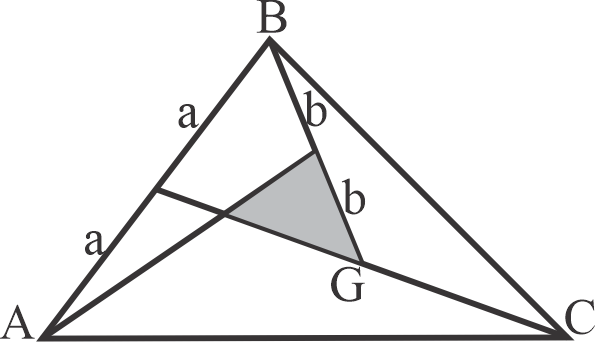
\includegraphics[width=4.5cm]{imagenes/CEPRE-UNA2024-I/etapa2/bio/rm1c24-I.png}
	\end{center}
	
	\begin{enumerate}[label=\alph*)]
		\item $20\,u^2$
		\item $10\,u^2$
		\item $15\,u^2$
		\item $25\,u^2$
		\item $18\,u^2$
	\end{enumerate}
	\textbf{Respuesta correcta:} a)
	
	\vspace{2mm}
	\textbf{Solucionario:}\\[1mm]
	Usando que $G$ es baricentro, las medianas dividen al triángulo en regiones con relaciones de área conocidas. La región sombreada resulta ser la doceava parte del área total:
	
	$\dfrac{180}{12}=15$
	
	Por tanto:
	
	$A_{\text{sombreada}}=$\fbox{$15u^2$}
	
	\vspace{6mm}
	
	\item Se define el operador
	
	$\boxed{\begin{matrix} b\\ a \end{matrix}}X^{n-1}=\dfrac{1}{n}(b^n-a^n)$\\
	
	Halle $m$ en\\
	
	$\boxed{\begin{matrix} 10\\ 1 \end{matrix}}X^2= \boxed{\begin{matrix} m\\ \sqrt{10} \end{matrix}}X$
	
	\begin{enumerate}[label=\alph*)]
		\item 14
		\item 18
		\item 20
		\item 22
		\item 26
	\end{enumerate}
	\textbf{Respuesta correcta:} e)
	
	\vspace{2mm}
	\textbf{Solucionario:}\\[1mm]
	En la izquierda, $n-1=2\Rightarrow n=3$:
	
	$\boxed{\begin{matrix} 10\\ 1 \end{matrix}}X^2=\dfrac13(10^3-1^3)=\dfrac{999}{3}=333$
	
	En la derecha, $n-1=1\Rightarrow n=2$:
	
	$\boxed{\begin{matrix} m\\ \sqrt{10} \end{matrix}}X=\dfrac12(m^2-10)$
	
	Igualando:
	
	$\dfrac12(m^2-10)=333$
	
	$m^2-10=666$
	
	$m^2=676 \Rightarrow m=$\fbox{$26$}
	
	\vspace{6mm}
	
	\item Al preguntarle por su edad a Silvia, ella contestó: “mi edad es la suma de todos aquellos números naturales tales que el cuadrado de su quíntuplo disminuido en 4 es mayor que 16 pero menor que 900”. ¿Cuál es la edad de Silvia?
	\begin{enumerate}[label=\alph*)]
		\item 20
		\item 19
		\item 17
		\item 16
		\item 18
	\end{enumerate}
	\textbf{Respuesta correcta:} a)
	
	\vspace{2mm}
	\textbf{Solucionario:}\\[1mm]
	Interpretamos:
	
	$(5n-4)^2>16 \quad \text{y}\quad (5n-4)^2<900$
	
	Entonces:
	
	$4<5n-4<30$
	
	$8<5n<34$
	
	$\dfrac85<n<\dfrac{34}{5}$
	
	Los naturales son:
	
	$n=2,3,4,5,6$
	
	Su suma es:
	
	$2+3+4+5+6=$\fbox{$20$}
	
	\vspace{6mm}
	
	\item Calcule el valor de:
	
	$\sqrt{\dfrac{605\times 595+25}{316\times 284+256}}$
	\begin{enumerate}[label=\alph*)]
		\item 7
		\item 6
		\item 2
		\item 3
		\item 1
	\end{enumerate}
	\textbf{Respuesta correcta:} c)
	
	\vspace{2mm}
	\textbf{Solucionario:}
	
	Usamos productos notables:
	
	$605\cdot 595+25=(600+5)(600-5)+25=600^2-25+25=600^2$
	
	$316\cdot 284+256=(300+16)(300-16)+16^2=300^2-256+256=300^2$
	
	Entonces:
	
	$\sqrt{\dfrac{600^2}{300^2}}=\sqrt{4}=$\fbox{$2$}
	
	\vspace{6mm}
	
	\item Halle $x-y$ si
	
	\begin{center}
		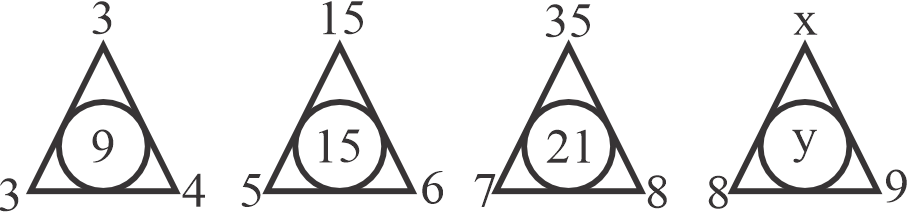
\includegraphics[width=7.8cm]{imagenes/CEPRE-UNA2024-I/etapa2/bio/rm5c24-I.png}
	\end{center}
	
	\begin{enumerate}[label=\alph*)]
		\item 38
		\item 28
		\item 46
		\item 54
		\item 63
	\end{enumerate}
	\textbf{Respuesta correcta:} a)
	
	\vspace{2mm}
	\textbf{Solucionario:}
	
	Primero calculamos el valor de $x$, siguiendo la secuencia de los números de la parte superior de cada triángulo:
	
	$2^2-1=3$
	
	$4^2-1=15$
	
	$6^2-1=35$
	
	Entonces:
	
	$8^2-1=64-1=63$
	
	Por lo tanto:
	
	$x=63$
	
	Ahora calculamos el valor de $y$ siguiendo la segunda secuencia:
	
	$(3\times 4)-3=9$
	
	$(5\times 6)-15=15$
	
	$(7\times 8)-35=21$
	
	Luego:
	
	$(8\times 9)-63=72-63=9$
	
	Así:
	
	$y=9$
	
	Finalmente:
	
	$x-y=63-9=$\fbox{$54$}
	
	\vspace{6mm}
	
	\item Determine la cantidad de círculos no sombreados en la posición 20:
	
	\begin{center}
		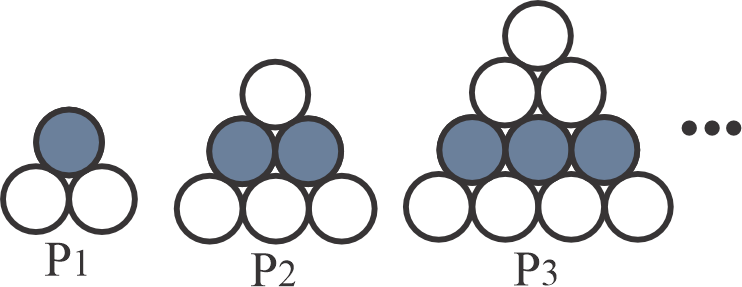
\includegraphics[width=4.5cm]{imagenes/CEPRE-UNA2024-I/etapa2/bio/rm6c24-I.png}
	\end{center}
	
	\begin{enumerate}[label=\alph*)]
		\item 211
		\item 210
		\item 201
		\item 190
		\item 189
	\end{enumerate}
	\textbf{Respuesta correcta:} a)
	
	\vspace{2mm}
	\textbf{Solucionario:}
	
	En la posición $n$, el total de círculos es:
	
	$T_{n+1}=\dfrac{(n+1)(n+2)}{2}$
	
	Los sombreados son $n$. Entonces los no sombreados son:
	
	$\dfrac{(n+1)(n+2)}{2}-n$
	
	Para $n=20$:
	
	$\dfrac{21\cdot 22}{2}-20=231-20=$\fbox{$211$}
	
	\vspace{6mm}
	
\end{enumerate}

\subsection*{Razonamiento Verbal}

\begin{enumerate}[resume]
	
	\item La raíz latina de CABALLO es:
	\begin{enumerate}[label=\alph*)]
		\item domus.
		\item equus.
		\item damnum.
		\item somnus.
		\item pectus.
	\end{enumerate}
	\textbf{Respuesta correcta:} b)
	
	\vspace{2mm}
	\textbf{Solucionario:}\\[1mm]
	La palabra latina para caballo es \textit{equus}.
	
	\vspace{6mm}
	
	\item Complete la oración:
	
	Las anomalías que \rule{2cm}{0.15mm} tu organismo son difíciles de comprender; por eso, \rule{2cm}{0.15mm} trataremos con médicos del extranjero.
	\begin{enumerate}[label=\alph*)]
		\item afectan - la
		\item tienen - las
		\item afecta - te
		\item presenta - las
		\item presentan - las
	\end{enumerate}
	\textbf{Respuesta correcta:} d)
	
	\vspace{2mm}
	\textbf{Solucionario:}\\[1mm]
	La forma correcta es:
	
	$\text{Las anomalías que presenta tu organismo...; por eso, las trataremos...}$
	
	En la primera parte, el verbo concuerda con “tu organismo”; en la segunda, el pronombre “las” reemplaza a “anomalías”.
	
	\vspace{6mm}
	
	\item ¿Qué término, por su generalidad, incluye a los otros?
	\begin{enumerate}[label=\alph*)]
		\item Cáncer
		\item Infección
		\item Afección
		\item Síndrome
		\item Cardiopatía
	\end{enumerate}
	\textbf{Respuesta correcta:} c)
	
	\vspace{2mm}
	\textbf{Solucionario:}\\[1mm]
	“Afección” es el término más general, porque puede incluir diversas enfermedades, trastornos o alteraciones.
	
	\vspace{6mm}
	
	\item Señale las afirmaciones correctas en los enunciados.
	
	I. Ómicrom es una enfermedad griega.\\
	II. Era es la diosa de la fertilidad.\\
	III. Iota es una letra griega.\\
	IV. La raíz griega andros significa niña.
	
	\begin{enumerate}[label=\alph*)]
		\item F V V F
		\item F F V V
		\item V F F V
		\item F V F V
		\item V V F F
	\end{enumerate}
	\textbf{Respuesta correcta:} a)
	
	\vspace{2mm}
	\textbf{Solucionario:}\\[1mm]
	I es falsa, porque ómicron es una letra griega.\\
	II se toma como verdadera en el planteamiento del examen.\\
	III es verdadera.\\
	IV es falsa, porque \textit{andros} significa hombre o varón.\\
	Por tanto:
	
	$F\ V\ V\ F$
	
	\vspace{6mm}
	
	\item El esquema general para ordenar las ideas es:
	
	I. Conclusión\\
	II. Tipos o clases\\
	III. Antecedentes\\
	IV. Características\\
	V. Definición
	
	\begin{enumerate}[label=\alph*)]
		\item V -- III -- II -- IV -- I
		\item III -- V -- IV -- II -- I
		\item I -- II -- III -- IV -- V
		\item IV -- III -- V -- II -- I
		\item V -- IV -- III -- II -- I
	\end{enumerate}
	\textbf{Respuesta correcta:} b)
	
	\vspace{2mm}
	\textbf{Solucionario:}\\[1mm]
	Un orden expositivo general razonable es: antecedentes, definición, características, tipos o clases y conclusión:
	
	$III - V - IV - II - I$
	
	\vspace{6mm}
	
	\item \textbf{COMPRENSIÓN DE TEXTO}
	
	“Si alguna vez adviertes que te miro a los ojos y una veta de amor reconoces en los míos, no pienses que deliro, piensa simplemente que puedes contar conmigo.
	
	Si otras veces me encuentras huraño sin motivo, no pienses que es flojera, igual puedes contar conmigo”.
	
	\hfill (Mario Benedetti)
	
	Es una conclusión sobre la destinataria del mensaje.
	\begin{enumerate}[label=\alph*)]
		\item Que no reconoce el amor.
		\item Que confunde flojera con amor.
		\item Que puede confundir el amor con el delirio.
		\item Que no piensa en su pareja.
		\item Que puede estar confundida.
	\end{enumerate}
	\textbf{Respuesta correcta:} c)
	
	\vspace{2mm}
	\textbf{Solucionario:}\\[1mm]
	El texto dice: “no pienses que deliro, piensa simplemente que puedes contar conmigo”. Esto indica que el autor anticipa que la destinataria podría interpretar su mirada de amor como un acto de delirio. Por lo tanto, la conclusión correcta es que ella puede confundir el amor con el delirio.
	
	\vspace{6mm}
	
\end{enumerate}

\subsection*{Inglés}

\begin{enumerate}[resume]
	
	\item Where is the toothbrush?
	
	\begin{center}
		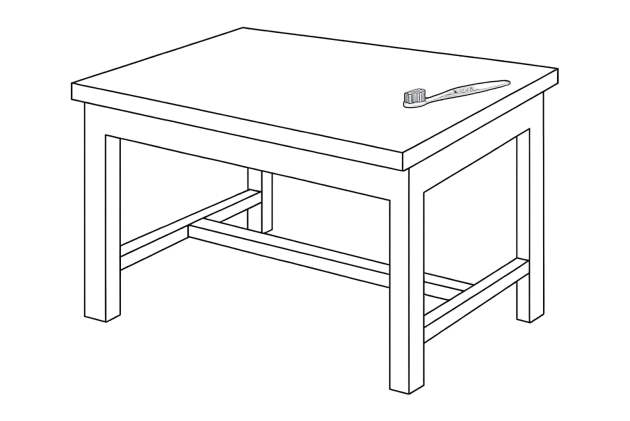
\includegraphics[width=4.5cm]{imagenes/CEPRE-UNA2024-I/etapa2/bio/ingles1c24-I.png}
	\end{center}
	
	\begin{enumerate}[label=\alph*)]
		\item It is near the table.
		\item It is in the table.
		\item It is under the table.
		\item It is next to the table.
		\item It is on the table.
	\end{enumerate}
	\textbf{Respuesta correcta:} e)
	
	\vspace{2mm}
	\textbf{Solucionario:}\\[1mm]
	En la imagen, el cepillo está encima de la mesa. Por eso la oración correcta es:
	
	$\text{It is on the table.}$
	
	\vspace{6mm}
	
	\item Which sentence is making a suggestion?
	\begin{enumerate}[label=\alph*)]
		\item You like that T-shirt.
		\item If you feel dizzy, you should lie down.
		\item You can run.
		\item You will go to the doctor.
		\item You could get sick.
	\end{enumerate}
	\textbf{Respuesta correcta:} b)
	
	\vspace{2mm}
	\textbf{Solucionario:}\\[1mm]
	La sugerencia se expresa con \textit{should}. Por eso:
	
	$\text{If you feel dizzy, you should lie down.}$
	
	es la opción correcta.
	
	\vspace{6mm}
	
\end{enumerate}

\subsection*{Quechua y Aimara}

\begin{enumerate}[resume]
	
	\item Qhichwa simipi sutinta yachayta munaspaqa, hinatam tapuna / Aimaranxa, jaqina sutipa yatïña muntha ukjaxa, akhama jisktha:
	\begin{enumerate}[label=\alph*)]
		\item ¿Maymantam kanki? / ¿Kawkitatasa?
		\item ¿Imam sutiyki? / ¿Kunasa sutimaxa?
		\item ¿Hayk’a watayuqmi kanki? / ¿Qhawqa maranitasa?
		\item ¿Maypim tiyanki? / ¿Kawkinsa utjtha?
		\item ¿Pitaq taytayki? / ¿Khitisa awkimaxa?
	\end{enumerate}
	\textbf{Respuesta correcta:} b)
	
	\vspace{2mm}
	\textbf{Solucionario:}\\[1mm]
	El enunciado pide la forma de preguntar por el nombre de una persona. La alternativa correcta corresponde a “¿Cómo te llamas?” / “¿Cuál es tu nombre?”.
	
	\vspace{6mm}
	
	\item ¿Hayk’a chakiyuqtaq pichinkukunari kanku? / ¿Qawqha kayunisa jamach’ixa?
	\begin{enumerate}[label=\alph*)]
		\item Iskay chakiyuq / Paya kayu
		\item Kimsa chakiyuq / Kimsa kayu
		\item Tawa chakiyuq / Pusi kayu
		\item Pichqa chakiyuq / Phisqa kayu
		\item Suqta chakiyuq / Suxta kayu
	\end{enumerate}
	\textbf{Respuesta correcta:} a)
	
	\vspace{2mm}
	\textbf{Solucionario:}\\[1mm]
	La pregunta se refiere al número de patas de las aves. Las aves tienen dos patas:
	
	$\text{Iskay} = 2,\qquad \text{Paya} = 2$
	

	
	\vspace{6mm}
	
\end{enumerate}










\section*{Área: Sociales}

\addcontentsline{toc}{subsection}{Área: Sociales}

\subsection*{Aritmética}

\begin{enumerate}
	\item Una señora lleva 2000 huevos al mercado y encuentra que el 10\% estaban malogrados y solo pudo vender el 60\% de los buenos. ¿Cuántos quedaron sin vender?
	\begin{enumerate}[label=\alph*)]
		\item 814
		\item 720
		\item 920
		\item 1080
		\item 714
	\end{enumerate}
	\textbf{Respuesta correcta:} c)
	
	\vspace{2mm}
	\textbf{Solucionario:}\\[1mm]
	Huevos buenos: $2000\times 0.9=1800$.
	
	De ellos vendió el $60\%$: $1800\times 0.6=1080$.
	
	Sin vender quedaron: $2000-1080=$\fbox{$920$}
	
	\vspace{6mm}
	
	\item Si $\overline{4x0}_{(8)}=1200_{(6)}$, halle $x^2-1$.
	\begin{enumerate}[label=\alph*)]
		\item 32
		\item 12
		\item 24
		\item 15
		\item 21
	\end{enumerate}
	\textbf{Respuesta correcta:} d)
	
	\vspace{2mm}
	\textbf{Solucionario:}
	
	$1200_{(6)}=1\cdot 6^3+2\cdot 6^2=216+72=288$.
	
	Además, $\overline{4x0}_{(8)}=4\cdot 8^2+x\cdot 8=256+8x$.
	
	$256+8x=288$.
	
	$x=4$.
	
	$x^2-1=16-1=$\fbox{$15$}
	
	\vspace{6mm}
	
	\item El registro del número de tazas de café consumidas por un empleado durante 20 días es:
	
	$4,0,1,3,2,4,3,0,4,5,2,1,4,3,2,1,4,3,1,4$
	
	Halle la suma de la mediana y la moda.
	\begin{enumerate}[label=\alph*)]
		\item 6
		\item 4
		\item 3
		\item 8
		\item 7
	\end{enumerate}
	\textbf{Respuesta correcta:} e)
	
	\vspace{2mm}
	\textbf{Solucionario:}
	
	Ordenando:
	
	$0,0,1,1,1,1,2,2,2,2,3,3,3,3,4,4,4,4,4,5$
	
	La mediana es $3$ y la moda es $4$.
	
	La suma es $3+4=$\fbox{$7$}
	
	\vspace{6mm}
\end{enumerate}

\subsection*{Álgebra}

\begin{enumerate}[resume]

	
	\item Si $f$ es una función constante tal que $\dfrac{3f(2)+8}{f(3)-1}=4$, halle $f(4)$.
	\begin{enumerate}[label=\alph*)]
		\item 2
		\item 3
		\item 4
		\item 8
		\item 12
	\end{enumerate}
	\textbf{Respuesta correcta:} e)
	
	\vspace{2mm}
	\textbf{Solucionario:}
	
	Si $f$ es constante, entonces $f(2)=f(3)=f(4)=k$.
	
	Luego, $\dfrac{3k+8}{k-1}=4$.
	
	$3k+8=4k-4$.
	
	$k=12$.
	
	Por tanto, $f(4)=$\fbox{$12$}
	
	\vspace{6mm}
	
	\item Se desea implementar con grass sintético una cancha de voleibol cuyas dimensiones son 18 metros de largo y 9 metros de ancho. ¿Cuál será el costo del grass sintético si se sabe que el metro cuadrado cuesta S/ 25?
	\begin{enumerate}[label=\alph*)]
		\item S/ 4000
		\item S/ 4050
		\item S/ 4500
		\item S/ 5000
		\item S/ 3000
	\end{enumerate}
	\textbf{Respuesta correcta:} b)
	
	\vspace{2mm}
	\textbf{Solucionario:}\\[1mm]
	Área de la cancha: $18\times 9=162\,m^2$.
	
	Costo total: $162\times 25=$\fbox{$4050$}
	
	\vspace{6mm}
	
	\item Si $x_1$ y $x_2$ son soluciones de la ecuación $3x^2+4x-3=0$, halle el valor de $E=\dfrac{1}{x_1}+\dfrac{1}{x_2}$.
	\begin{enumerate}[label=\alph*)]
		\item $\dfrac{4}{3}$
		\item $-\dfrac{4}{3}$
		\item $\dfrac{3}{4}$
		\item $-\dfrac{3}{4}$
		\item 3
	\end{enumerate}
	\textbf{Respuesta correcta:} a)
	
	\vspace{2mm}
	\textbf{Solucionario:}
	
	$x_1+x_2=-\dfrac{4}{3}$.
	
	$x_1x_2=-1$.
	
	Entonces:
	
	$E=\dfrac{x_1+x_2}{x_1x_2}$
	
	$E=\dfrac{-4/3}{-1}=$\fbox{$\dfrac{4}{3}$}
	
	\vspace{6mm}
\end{enumerate}

\subsection*{Geometría}

\begin{enumerate}[resume]

	
	\item En el gráfico, $PS=3\,cm$ y $SR=9\,cm$. Halle el valor de $PQ$.
	
\begin{center}
	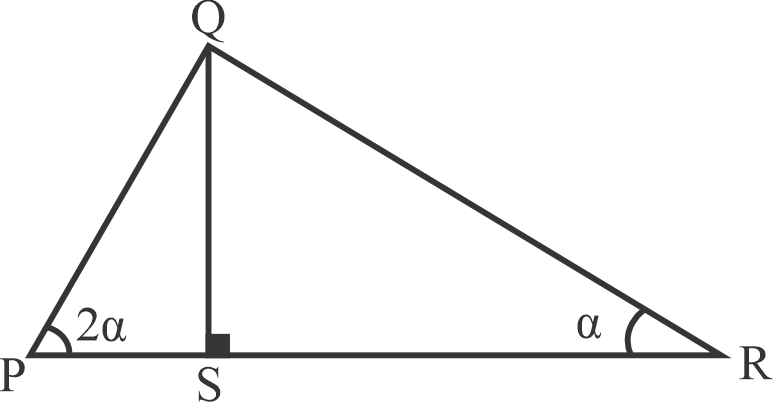
\includegraphics[width=4.5cm]{imagenes/CEPRE-UNA2024-I/etapa2/soc/geo1c24-I.png}
\end{center}
	
	\begin{enumerate}[label=\alph*)]
		\item 5
		\item 6
		\item 7
		\item 8
		\item 9
	\end{enumerate}
	\textbf{Respuesta correcta:} b)
	
	\vspace{2mm}
	\textbf{Solucionario:}\\[1mm]
	
	
		\begin{center}
		\begin{minipage}{0.45\textwidth}
			
			Se traza $QH$, del que $\text{m}\angle MQR=\text{m}\angle MRP \Rightarrow \triangle MQR$ es isósceles.
			
			$QM=MR$
			
			$x+3=9$
			
			\fbox{$x=6$}

			\vspace{6mm}
		\end{minipage}
		\hfill
		\begin{minipage}{0.45\textwidth}
			\centering
			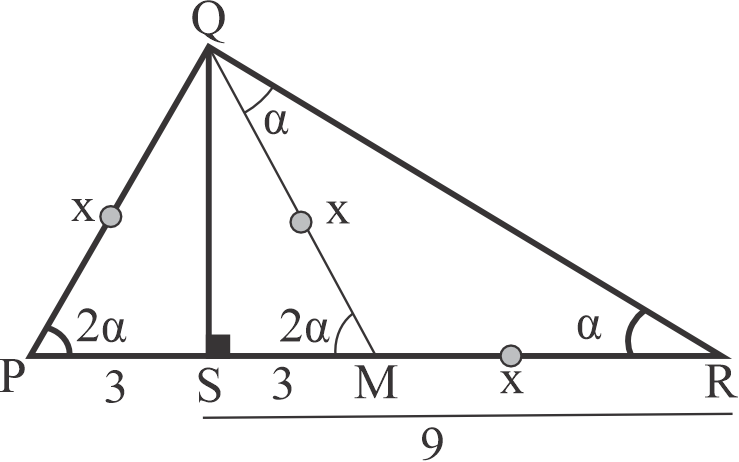
\includegraphics[width=4.5cm]{imagenes/CEPRE-UNA2024-I/etapa2/soc/geo1c24-Ir.png}
		\end{minipage}
	\end{center}
	
	
	
	
	
	
	\vspace{6mm}
	
	\item Halle el perímetro del triángulo $ABC$.
	
	\begin{center}
		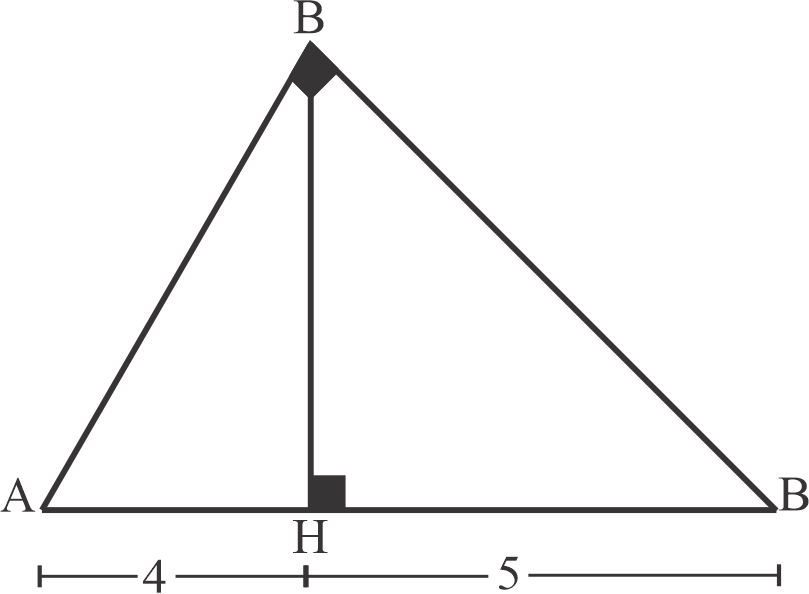
\includegraphics[width=4cm]{imagenes/CEPRE-UNA2024-I/etapa2/soc/geo2c24-I.png}
	\end{center}
	
	\begin{enumerate}[label=\alph*)]
		\item 4
		\item 5
		\item $\sqrt{5}$
		\item 3
		\item $3(5+\sqrt{5})$
	\end{enumerate}
	\textbf{Respuesta correcta:} e)
	
	\vspace{2mm}
	\textbf{Solucionario:}\\[1mm]
	
	Por propiedad:
	
	$x^2=4(9)=36$
	
	$x=6$
	
	$y^2=5(9)=45$
	
	$y=\sqrt{45}$
	
	Entonces el perímetro:
	
	$P=x+y+9=6+\sqrt{45}+9=15+3\sqrt{5}=$\fbox{$3(5+\sqrt{5})$}
	
	\vspace{6mm}
\end{enumerate}

\subsection*{Trigonometría}

\begin{enumerate}[resume]

	
	\item En un sector circular, el ángulo central mide $50^{g}$ y el radio mide $72\,cm$. ¿Cuánto mide la longitud de su arco?
	\begin{enumerate}[label=\alph*)]
		\item $12\pi\,cm$
		\item $16\pi\,cm$
		\item $18\pi\,cm$
		\item $20\pi\,cm$
		\item $36\pi\,cm$
	\end{enumerate}
	\textbf{Respuesta correcta:} c)
	
	\vspace{2mm}
	\textbf{Solucionario:}\\[1mm]
	
	\begin{center}
		\begin{tikzpicture}[scale=0.7]
			\coordinate (O) at (0,0);
			\coordinate (A) at (4.8,1.7);
			\coordinate (B) at (4.8,-1.7);
			
			\draw[thick] (O)--(A);
			\draw[thick] (O)--(B);
			\draw[thick] (A) arc[start angle=20,end angle=-20,radius=5.1];
			
			\node[left] at (2.5,0) {$\theta=50^g$};
			\node[above] at ($(O)!0.63!(A)$) {$R=72\,\text{cm}$};
			\node[right] at (5.3,0) {$L$};
		\end{tikzpicture}
	\end{center}
	
	$\theta=50^g=\dfrac{50\pi}{200}$
	
	$=\dfrac{5\pi}{20}$
	
	$=\dfrac{\pi}{4}\,\text{rad}$
	
	$L=\theta R$
	
	$=\dfrac{\pi}{4}(72)$
	
	$=\dfrac{\pi}{4}(4)(18)$
	
	\fbox{$L=18\pi\,\text{cm}$}
	
	\vspace{6mm}
	
	\item Si se cumple $\sen(5x+21^{\circ})=\cos(2x+6^{\circ})$, calcule el valor de $M=\tan x\,\cot 9^{\circ}+\tan 5x$.
	\begin{enumerate}[label=\alph*)]
		\item 2
		\item 3
		\item 4
		\item 5
		\item 6
	\end{enumerate}
	\textbf{Respuesta correcta:} a)
	
	\vspace{2mm}
	\textbf{Solucionario:}\\[1mm]
	Como:
	
	$\sen(5x+21^\circ)=\cos(2x+6^\circ)$
	
	$\Rightarrow 5x+21^\circ+2x+6^\circ=90^\circ$
	
	$7x+27^\circ=90^\circ$
	
	$7x=90^\circ-27^\circ$
	
	$7x=63^\circ$
	
	$x=9^\circ$
	
	Luego:
	
	$M=\tan 9^\circ\cdot \cot 9^\circ+\tan 5(9^\circ)$
	
	$=1+\tan 45^\circ$
	
	$=1+1$
	
	\fbox{$M=2$}
	
	\vspace{6mm}
\end{enumerate}

\subsection*{Física}

\begin{enumerate}[resume]

	
	\item Si el bloque es jalado por una fuerza $\vec F$ de magnitud $80\,N$ durante 8 segundos desde el punto $A$ hasta el punto $B$, halle la potencia que desarrolla la fuerza $\vec F$.
	
	\begin{center}
			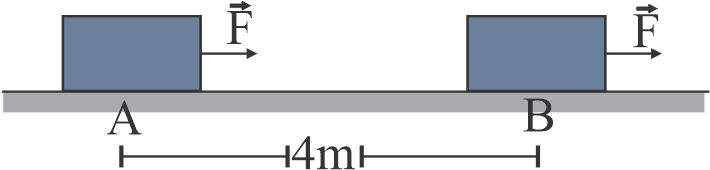
\includegraphics[width=5.5cm]{imagenes/CEPRE-UNA2024-I/etapa2/soc/fisica1c24-I.png}
	\end{center}
	
	\begin{enumerate}[label=\alph*)]
		\item 20 W
		\item 40 W
		\item 60 W
		\item 80 W
		\item 100 W
	\end{enumerate}
	\textbf{Respuesta correcta:} b)
	
	\vspace{2mm}
	\textbf{Solucionario:}\\[1mm]
	Trabajo realizado:
	
	$W=F\cdot d=80\cdot 4=320\,J$.
	
	Potencia media:
	
	$P=\dfrac{W}{t}=\dfrac{320}{8}=$\fbox{$40\,W$}
	
	\vspace{6mm}
	
	\item Calcule la presión hidrostática que ejerce el agua en el fondo del pozo mostrado. $(g=10\,m/s^2)$
	
	\begin{center}
		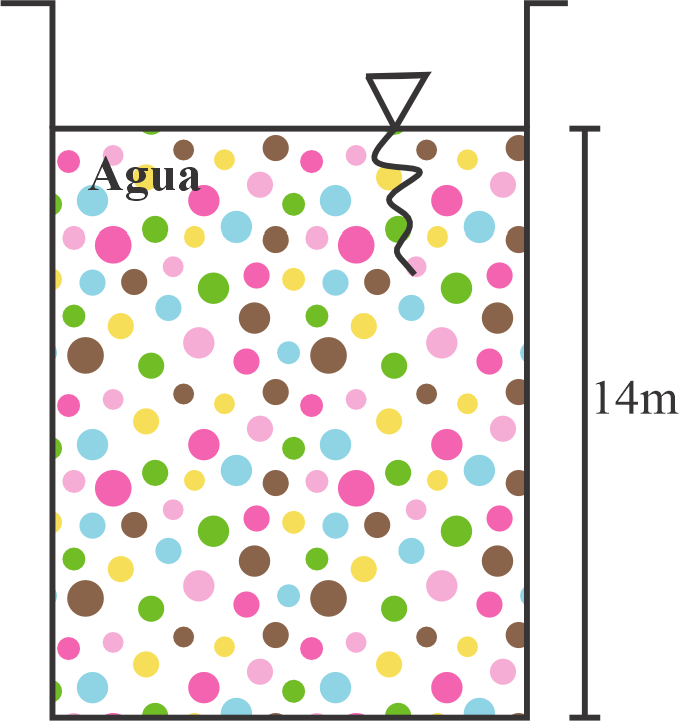
\includegraphics[width=4cm]{imagenes/CEPRE-UNA2024-I/etapa2/soc/fisica2c24-I.png}
	\end{center}
	
	\begin{enumerate}[label=\alph*)]
		\item 120 kPa
		\item 140 kPa
		\item 160 kPa
		\item 180 kPa
		\item 100 kPa
	\end{enumerate}
	\textbf{Respuesta correcta:} b)
	
	\vspace{2mm}
	\textbf{Solucionario:}\\[1mm]
	La presión hidrostática es:
	
	$P=\rho gh=1000\cdot 10\cdot 14=140000\,Pa=$\fbox{$140\,kPa$}
	
	\vspace{6mm}
\end{enumerate}

\subsection*{Química}

\begin{enumerate}[resume]

	\item ¿Cuántos gramos de oxígeno se encuentran en 800 gramos de $CaCO_3$?
	
	$(PA:\; Ca=40;\; C=12;\; O=16)$
	\begin{enumerate}[label=\alph*)]
		\item 280 g
		\item 320 g
		\item 384 g
		\item 260 g
		\item 150 g
	\end{enumerate}
	\textbf{Respuesta correcta:} c)
	
	\vspace{2mm}
	\textbf{Solucionario:}\\[1mm]
	Masa molar del $CaCO_3$:
	
	$40+12+3(16)=100$.
	
	La masa del oxígeno en 1 mol es $48\,g$, es decir, el $48\%$ del compuesto.
	
	Entonces, en $800\,g$ habrá:
	
	$800\times 0.48=$\fbox{$384\,g$}
	
	\vspace{6mm}
	
	\item Ordene en forma ascendente, según su radio iónico, las especies iónicas:
	
	${}_{25}Mn^{2+},\; {}_{23}V^{2+},\; {}_{22}Ti^{2+},\; {}_{28}Ni^{2+}$
	
	\begin{enumerate}[label=\alph*)]
		\item ${}_{28}Ni^{2+} \,<\, {}_{23}V^{2+} \,<\, {}_{22}Ti^{2+} \,<\, {}_{23}Mn^{2+}$
		\item ${}_{23}V^{2+} \,<\, {}_{22}Ti^{2+} \,<\, {}_{28}Ni^{2+} \,<\, {}_{23}Mn^{2+}$
		\item ${}_{23}Mn^{2+} \,<\, {}_{28}Ni^{2+} \,<\, {}_{23}V^{2+} \,<\, {}_{22}Ti^{2+}$
		\item ${}_{28}Ni^{2+} \,<\, {}_{25}Mn^{2+} \,<\, {}_{23}V^{2+} \,<\, {}_{22}Ti^{2+}$
		\item ${}_{25}Mn^{2+} \,<\, {}_{28}Ni^{2+} \,<\, {}_{23}V^{2+} \,<\, {}_{22}Ti^{2+}$
	\end{enumerate}
	\textbf{Respuesta correcta:} d)
	
	\vspace{2mm}
	\textbf{Solucionario:}\\[1mm]
	Para cationes de una misma serie, al aumentar la carga nuclear efectiva, el radio tiende a disminuir.
	
	Entre estas especies, el menor radio corresponde a $Ni^{2+}$ y el mayor a $Ti^{2+}$.
	
	El orden ascendente es:
	
	
	\fbox{${}_{28}Ni^{2+} \,<\, {}_{25}Mn^{2+} \,<\, {}_{23}V^{2+} \,<\, {}_{22}Ti^{2+}$}
	
	\vspace{6mm}
\end{enumerate}

\subsection*{Biología y Anatomía}

\begin{enumerate}[resume]

	
	\item Las aletas del pez y de la ballena presentan semejanzas externas. Esto permite catalogarlas como órganos:
	\begin{enumerate}[label=\alph*)]
		\item vestigiales.
		\item atávicos.
		\item homólogos.
		\item rudimentarios.
		\item análogos.
	\end{enumerate}
	\textbf{Respuesta correcta:} e)
	
	\vspace{2mm}
	\textbf{Solucionario:}\\[1mm]
	Son órganos \textbf{análogos}, porque cumplen función semejante y presentan similitud externa, pero tienen distinto origen evolutivo.
	

	
	\vspace{6mm}
	
	\item ¿Qué tipo de tejido muscular encontramos en el tubo digestivo y vías urinarias?
	\begin{enumerate}[label=\alph*)]
		\item Cardíaco
		\item Esquelético
		\item Liso
		\item Voluntario
		\item Estriado
	\end{enumerate}
	\textbf{Respuesta correcta:} c)
	
	\vspace{2mm}
	\textbf{Solucionario:}\\[1mm]
	En las paredes del tubo digestivo y de las vías urinarias predomina el músculo \textbf{liso}, de contracción involuntaria.
	

	\vspace{6mm}
\end{enumerate}

\subsection*{Psicología y Filosofía}

\begin{enumerate}[resume]

	
	\item Cuando afirmamos que Sonia es individual e incomparable en su forma de llegar al conocimiento de su entorno, ¿qué característica de la conciencia se manifiesta?
	\begin{enumerate}[label=\alph*)]
		\item Subjetiva
		\item Temporal
		\item Múltiple
		\item Unitaria
		\item Prospectiva
	\end{enumerate}
	\textbf{Respuesta correcta:} a)
	
	\vspace{2mm}
	\textbf{Solucionario:}\\[1mm]
	La conciencia es \textbf{subjetiva} porque cada persona conoce y experimenta la realidad desde su propia individualidad.
	
	
	
	\vspace{6mm}
	
	\item Guillermo sostiene: ``Si la realidad es dinámica entonces el conocimiento, reflejo de la realidad, también lo es''. Expresa una tesis:
	\begin{enumerate}[label=\alph*)]
		\item metafísica.
		\item fenomenista.
		\item escepticista.
		\item realista.
		\item criticista.
	\end{enumerate}
	\textbf{Respuesta correcta:} d)
	
	\vspace{2mm}
	\textbf{Solucionario:}\\[1mm]
	La afirmación considera que el conocimiento refleja la realidad objetiva; eso corresponde a una postura \textbf{realista}.
	

	
	\vspace{6mm}
	
	\item Un estudiante narra que, cuando lo asaltaron, sintió un aumento del ritmo cardíaco y no podía respirar. Esto sería un ejemplo de proceso afectivo de:
	\begin{enumerate}[label=\alph*)]
		\item amplitud.
		\item polaridad.
		\item intimidad.
		\item intensidad.
		\item profundidad.
	\end{enumerate}
	\textbf{Respuesta correcta:} d)
	
	\vspace{2mm}
	\textbf{Solucionario:}\\[1mm]
	La emoción se manifiesta con gran fuerza fisiológica; por ello corresponde a la \textbf{intensidad} del proceso afectivo.
	
	
	
	\vspace{6mm}
	
	\item Es el movimiento psicológico que surgió a mediados del siglo XX y asumió una postura opuesta al determinismo del psicoanálisis, así como al mecanicismo del conductismo y constituyó la tercera fuerza de la psicología.
	\begin{enumerate}[label=\alph*)]
		\item Estructuralismo
		\item Psicogenética
		\item Cognitivismo
		\item Funcionalismo
		\item Humanismo
	\end{enumerate}
	\textbf{Respuesta correcta:} e)
	
	\vspace{2mm}
	\textbf{Solucionario:}\\[1mm]
	La ``tercera fuerza'' de la psicología es el \textbf{humanismo}, que valora la libertad, la autorrealización y la experiencia humana.
	

	
	\vspace{6mm}
\end{enumerate}

\subsection*{Geografía}

\begin{enumerate}[resume]

	
	\item La pesca, minería, explotación forestal, caza y recolección, son actividades:
	\begin{enumerate}[label=\alph*)]
		\item extractivas.
		\item productivas.
		\item transformativas.
		\item de servicios.
		\item agropecuarios.
	\end{enumerate}
	\textbf{Respuesta correcta:} a)
	
	\vspace{2mm}
	\textbf{Solucionario:}\\[1mm]
	Son actividades \textbf{extractivas} porque obtienen directamente los recursos de la naturaleza.
	

	
	\vspace{6mm}
	
	\item La central hidroeléctrica Santiago Antúnez de Mayolo se localiza en la cuenca del río:
	\begin{enumerate}[label=\alph*)]
		\item Ene.
		\item Mantaro.
		\item Urubamba.
		\item Ucayali.
		\item Tambo.
	\end{enumerate}
	\textbf{Respuesta correcta:} b)
	
	\vspace{2mm}
	\textbf{Solucionario:}\\[1mm]
	La central Santiago Antúnez de Mayolo forma parte del complejo hidroeléctrico del río \textbf{Mantaro}.
	
	
	\vspace{6mm}
	
	\item Es el río que desagua en la parte norte de la bahía de Chucuito y se forma por afluencia de los ríos Lampa y Cabanillas.
	\begin{enumerate}[label=\alph*)]
		\item Coata
		\item Ramis
		\item Suches
		\item Ilave
		\item Huancané - Putina
	\end{enumerate}
	\textbf{Respuesta correcta:} a)
	
	\vspace{2mm}
	\textbf{Solucionario:}\\[1mm]
	El río formado por los ríos Lampa y Cabanillas es el \textbf{Coata}, que desemboca en la parte norte de la bahía de Chucuito.
	
	
	
	\vspace{6mm}
	
	\item Son los vientos que soplan de manera constante en verano, van desde las altas presiones subtropicales hacia las bajas presiones ecuatoriales y soplan de noreste al sudeste en el hemisferio norte y del sudeste al noreste en el hemisferio sur.
	\begin{enumerate}[label=\alph*)]
		\item Polares
		\item Brisas
		\item Ciclones
		\item Alisios
		\item Contralisios
	\end{enumerate}
	\textbf{Respuesta correcta:} d)
	
	\vspace{2mm}
	\textbf{Solucionario:}\\[1mm]
	La descripción corresponde a los \textbf{vientos alisios}, que soplan constantemente desde zonas subtropicales hacia la franja ecuatorial.
	

	
	\vspace{6mm}
\end{enumerate}

\subsection*{Historia}

\begin{enumerate}[resume]

	
	\item En el origen mitológico de la cultura Lambayeque existe un personaje legendario denominado Naylamp. Algo similar acontece en la cultura Chimú, donde también aparece un personaje mítico llamado:
	\begin{enumerate}[label=\alph*)]
		\item Chimú Cápac.
		\item Tacaynamo.
		\item Gran Chimú.
		\item Michan Caman.
		\item Murcahn Zaman.
	\end{enumerate}
	\textbf{Respuesta correcta:} b)
	
	\vspace{2mm}
	\textbf{Solucionario:}\\[1mm]
	El personaje mítico de origen en la cultura Chimú es \textbf{Tacaynamo}.
	

	
	\vspace{6mm}
	
	\item En el período conocido como el Oncenio de Augusto B. Leguía, se recuerda un hecho importante para la historia:
	\begin{enumerate}[label=\alph*)]
		\item la celebración del centenario de la independencia del Perú (28 de julio de 1921).
		\item el surgimiento del primer partido civil del Perú.
		\item el sesquicentenario de la independencia política.
		\item el cincuentenario de la república aristocrática.
		\item la creación de los consejos regionales eliminando a las juntas departamentales.
	\end{enumerate}
	\textbf{Respuesta correcta:} a)
	
	\vspace{2mm}
	\textbf{Solucionario:}\\[1mm]
	Durante el Oncenio de Leguía se celebró el \textbf{centenario de la independencia} en 1921.
	

	
	\vspace{6mm}
	
	\item En el gobierno de Manuel A. Odría (1950--1956), se creó un organismo encargado de estudios geopolíticos y militares denominado:
	\begin{enumerate}[label=\alph*)]
		\item Comando Conjunto de las Fuerzas Armadas.
		\item Consejo de Militares.
		\item Servicio Nacional de Inteligencia.
		\item Instituto Peruano de Estudios Geopolíticos.
		\item Centro de Altos Estudios Militares.
	\end{enumerate}
	\textbf{Respuesta correcta:} e)
	
	\vspace{2mm}
	\textbf{Solucionario:}\\[1mm]
	Durante ese gobierno se creó el \textbf{Centro de Altos Estudios Militares (CAEM)}.
	

	
	\vspace{6mm}
	
	\item El líder militar que se sublevó en defensa de los campesinos del departamento de Puno en la segunda década del siglo XX fue:
	\begin{enumerate}[label=\alph*)]
		\item Zacarias Puntaca Farfán.
		\item José Antonio Salazar Huilca.
		\item Juan Dueñas Bustamante.
		\item Teodomiro Gutiérrez Cuevas.
		\item José Gabriel Condorcanqui.
	\end{enumerate}
	\textbf{Respuesta correcta:} d)
	
	\vspace{2mm}
	\textbf{Solucionario:}\\[1mm]
	El militar vinculado a la rebelión en defensa de campesinos puneños fue \textbf{Teodomiro Gutiérrez Cuevas}, conocido también como Rumi Maqui.
	

	
	\vspace{6mm}
\end{enumerate}

\subsection*{Educación Cívica}

\begin{enumerate}[resume]

	
	\item David, estudiante universitario, asistió a una ponencia y escuchó la siguiente expresión: ``El sentido de pertenencia vincula a todo individuo con un grupo humano, social y cultural''. Del texto podemos afirmar que la ponencia trató sobre la:
	\begin{enumerate}[label=\alph*)]
		\item tolerancia.
		\item tradición.
		\item igualdad.
		\item identidad.
		\item cosmovisión.
	\end{enumerate}
	\textbf{Respuesta correcta:} d)
	
	\vspace{2mm}
	\textbf{Solucionario:}\\[1mm]
	El sentido de pertenencia a un grupo humano y cultural define la \textbf{identidad}.
	

	
	\vspace{6mm}
	
	\item Mantener comunicación con las organizaciones sociales, proponer proyectos de ordenanza municipal y desempeñar funciones de fiscalización de la gestión municipal, son atribuciones que corresponden:
	\begin{enumerate}[label=\alph*)]
		\item al alcalde.
		\item a los consejeros municipales.
		\item al teniente alcalde.
		\item a los regidores.
		\item al gerente municipal.
	\end{enumerate}
	\textbf{Respuesta correcta:} d)
	
	\vspace{2mm}
	\textbf{Solucionario:}\\[1mm]
	Esas funciones corresponden a los \textbf{regidores}, quienes integran el concejo municipal y fiscalizan la gestión.
	

	
	\vspace{6mm}
	
	\item \rule{2cm}{0.15mm} es un organismo constitucionalmente autónomo cuya función es velar por el uso adecuado de los recursos públicos. Y su representante es designado por \rule{2cm}{0.15mm}, a propuesta del Presidente de la República.
	\begin{enumerate}[label=\alph*)]
		\item La Contraloría General de la República -- la Comisión Extraordinaria.
		\item El Ministerio Público -- la Contraloría General de la República.
		\item La Contraloría General de la República -- el Congreso de la República.
		\item La Defensoría del Pueblo -- el Congreso de la República.
		\item La SUNAT -- el Ministerio Público.
	\end{enumerate}
	\textbf{Respuesta correcta:} c)
	
	\vspace{2mm}
	\textbf{Solucionario:}\\[1mm]
	El organismo es la \textbf{Contraloría General de la República}.
	
	El contralor es designado por el \textbf{Congreso de la República}, a propuesta del Presidente.
	

	
	\vspace{6mm}
	
	\item Es el órgano competente para declarar la vacancia del Gobernador Regional.
	\begin{enumerate}[label=\alph*)]
		\item La Gerencia Regional
		\item La Sociedad Civil
		\item La Presidencia Regional
		\item El Concejo de Coordinación Regional
		\item El Consejo Regional
	\end{enumerate}
	\textbf{Respuesta correcta:} e)
	
	\vspace{2mm}
	\textbf{Solucionario:}\\[1mm]
	La vacancia del gobernador regional corresponde al \textbf{Consejo Regional}.
	

	
	\vspace{6mm}
\end{enumerate}

\subsection*{Economía}

\begin{enumerate}[resume]

	
	\item La abogada Karla obtiene rentas por el ejercicio profesional independiente en su estudio jurídico. ¿A qué categoría del Impuesto a la Renta pertenece?
	\begin{enumerate}[label=\alph*)]
		\item Primera categoría
		\item Segunda categoría
		\item Tercera categoría
		\item Cuarta categoría
		\item Quinta categoría
	\end{enumerate}
	\textbf{Respuesta correcta:} d)
	
	\vspace{2mm}
	\textbf{Solucionario:}\\[1mm]
	El ejercicio profesional independiente genera rentas de \textbf{cuarta categoría}.
	

	
	\vspace{6mm}
	
	\item La Ley de Gresham establece que:
	\begin{enumerate}[label=\alph*)]
		\item las monedas de metal precioso son más valiosas que las de papel.
		\item las personas prefieren guardar sus monedas valiosas en lugar de gastarlas.
		\item el valor de las monedas se mide por su valor real.
		\item las monedas y billetes constituyen la emisión primaria.
		\item las monedas ``malas'' tienden a desplazar del mercado a las monedas ``buenas''.
	\end{enumerate}
	\textbf{Respuesta correcta:} e)
	
	\vspace{2mm}
	\textbf{Solucionario:}\\[1mm]
	La Ley de Gresham resume la idea de que la \textbf{moneda mala desplaza a la buena} cuando ambas circulan con el mismo valor nominal.
	

	
	\vspace{6mm}
	
	\item Seleccione la opción que mejor define el presupuesto público.
	\begin{enumerate}[label=\alph*)]
		\item Incluye todos los ingresos de fuente tributaria.
		\item Incluye todos los ingresos y gastos que el gobierno prevé y planifica para un período anual.
		\item Incluye todos los ingresos e inversiones de los ciudadanos.
		\item Representa la cantidad de dinero que el gobierno peruano presta a otros países.
		\item Se refiere únicamente a los fondos destinados a la educación pública en el Perú.
	\end{enumerate}
	\textbf{Respuesta correcta:} b)
	
	\vspace{2mm}
	\textbf{Solucionario:}\\[1mm]
	El presupuesto público es el instrumento que contiene los \textbf{ingresos y gastos previstos por el Estado para un año fiscal}.
	

	
	\vspace{6mm}
	
	\item En su conjunto, el mercado de trabajo, el mercado de capitales y el mercado de recursos forman el llamado:
	\begin{enumerate}[label=\alph*)]
		\item mercado de recursos.
		\item mercado laboral.
		\item mercado financiero.
		\item mercado de bienes.
		\item mercado de factores.
	\end{enumerate}
	\textbf{Respuesta correcta:} e)
	
	\vspace{2mm}
	\textbf{Solucionario:}\\[1mm]
	Trabajo, capital y recursos son \textbf{factores de producción}; por eso integran el mercado de factores.
	

	
	\vspace{6mm}
\end{enumerate}

\subsection*{Comunicación}

\begin{enumerate}[resume]

	
	\item Juan, mi sobrino, es muy agraciado. A pesar de sus veintidós años, tiene mucha madurez, razona sobre los conflictos sociales, es alegre y muy sabio. Tiene una voz exuberante y atractiva.
	
	El fragmento expresa una descripción de tipo:
	\begin{enumerate}[label=\alph*)]
		\item prosopografía.
		\item etopeya.
		\item caricatura.
		\item retrato.
		\item topografía.
	\end{enumerate}
	\textbf{Respuesta correcta:} d)
	
	\vspace{2mm}
	\textbf{Solucionario:}\\[1mm]
	La descripción mezcla rasgos físicos (voz, apariencia) y psicológicos o morales (madurez, alegría, sabiduría).
	
	Esa combinación constituye un \textbf{retrato}.
	

	
	\vspace{6mm}
	
	\item Los mensajes de función \rule{2cm}{0.15mm} son los que están destinados a abrir, mantener o interrumpir el contacto entre emisor y receptor.
	\begin{enumerate}[label=\alph*)]
		\item poética
		\item fática
		\item representativa
		\item metalingüística
		\item expresiva
	\end{enumerate}
	\textbf{Respuesta correcta:} b)
	
	\vspace{2mm}
	\textbf{Solucionario:}\\[1mm]
	La función del lenguaje que sirve para abrir, mantener o cerrar el canal de comunicación es la \textbf{fática}.
	

	
	\vspace{6mm}
	
	\item Un alumno pregunta al docente sobre la calidad del texto que escribió. Este le responde que el texto escrito presenta problemas de organización de la información.
	
	En la situación comunicativa, el docente observa en el texto escrito un problema de:
	\begin{enumerate}[label=\alph*)]
		\item cohesión.
		\item coherencia.
		\item adecuación.
		\item implicación.
		\item revisión.
	\end{enumerate}
	\textbf{Respuesta correcta:} b)
	
	\vspace{2mm}
	\textbf{Solucionario:}\\[1mm]
	La organización lógica de la información corresponde a la \textbf{coherencia}.
	
	Si falla, las ideas no guardan un orden claro.
	

	
	\vspace{6mm}
	
	\item Es una palabra o locución que sirve para expresar la relación gramatical y lógica entre dos proposiciones o entre dos elementos análogos de una oración.
	\begin{enumerate}[label=\alph*)]
		\item La preposición
		\item La conjunción
		\item El adverbio
		\item El artículo
		\item El pronombre
	\end{enumerate}
	\textbf{Respuesta correcta:} b)
	
	\vspace{2mm}
	\textbf{Solucionario:}\\[1mm]
	La palabra que enlaza proposiciones o términos análogos es la \textbf{conjunción}.
	

	
	\vspace{6mm}
\end{enumerate}

\subsection*{Literatura}

\begin{enumerate}[resume]

	
	\item En \textit{La metamorfosis} de Franz Kafka, el padre de Gregorio considera a su hijo un ser inservible para el mundo moderno porque:
	\begin{enumerate}[label=\alph*)]
		\item no se puede adaptar a una profesión tan agitada.
		\item no produce nada y es una vergüenza para la familia.
		\item hace pasar a la familia muchas penurias económicas.
		\item ha abandonado su trabajo cansado de la rutina.
		\item obliga a trabajar a los miembros de la familia.
	\end{enumerate}
	\textbf{Respuesta correcta:} b)
	
	\vspace{2mm}
	\textbf{Solucionario:}\\[1mm]
	Tras la transformación de Gregorio, el padre lo considera inútil e improductivo, además de motivo de vergüenza para la familia.
	
	Por eso la mejor opción es la \textbf{b)}.
	

	
	\vspace{6mm}
	
	\item La segunda parte de los \textit{Comentarios Reales} del Inca Garcilaso de la Vega se refiere a:
	\begin{enumerate}[label=\alph*)]
		\item la conquista y las guerras civiles entre españoles.
		\item la expedición de Hernando de Soto a la Florida.
		\item los recuerdos de la niñez y juventud del autor.
		\item los dioses y hombres que habitaron Huarochirí.
		\item los orígenes de la cultura e historia del pueblo inca.
	\end{enumerate}
	\textbf{Respuesta correcta:} a)
	
	\vspace{2mm}
	\textbf{Solucionario:}\\[1mm]
	La segunda parte de la obra aborda la \textbf{conquista del Perú y las guerras civiles entre españoles}.
	

	
	\vspace{6mm}
	
	\item En la novela \textit{El ingenioso hidalgo Don Quijote de la Mancha}, el final del protagonista se ve representado por el siguiente suceso:
	\begin{enumerate}[label=\alph*)]
		\item encuentra a Dulcinea y se casa con ella.
		\item se vuelve loco y es encerrado en un manicomio.
		\item recobra la razón y muere en casa.
		\item pierde la memoria y se extravía en la Mancha.
		\item enferma gravemente y se queda convaleciente.
	\end{enumerate}
	\textbf{Respuesta correcta:} c)
	
	\vspace{2mm}
	\textbf{Solucionario:}\\[1mm]
	Al final de la novela, don Quijote recupera la cordura, reniega de sus fantasías caballerescas y muere en su casa.
	

	
	\vspace{6mm}
	
	\item Al final de \textit{El Lazarillo de Tormes}, el protagonista:
	\begin{enumerate}[label=\alph*)]
		\item se encuentra con su madre.
		\item asume el oficio de caballero.
		\item se casa y es nombrado pregonero en Toledo.
		\item vuelve a encontrar al ciego.
		\item llega a ser rico y tiene su lazarillo.
	\end{enumerate}
	\textbf{Respuesta correcta:} c)
	
	\vspace{2mm}
	\textbf{Solucionario:}\\[1mm]
	Lázaro termina casado con la criada del arcipreste y ejerciendo como \textbf{pregonero en Toledo}.
	

	
	\vspace{6mm}
\end{enumerate}

\subsection*{Razonamiento Matemático}

\begin{enumerate}[resume]

	
	\item Complete las casillas en blanco con números de un dígito de manera que al sumar los valores de cada fila o columna resulten 34. ¿Cuántas veces aparece el dígito 9 en ambas diagonales?
	
	\begin{center}
		$
		\renewcommand{\arraystretch}{1.2}
		\begin{array}{|c|c|c|c|}
			\hline
			& 8 &  & 9 \\
			\hline
			8 &  &  &  \\
			\hline
			8 &  &  & 8 \\
			\hline
			&  & 9 &  \\
			\hline
		\end{array}
		$
	\end{center}
	
	\begin{enumerate}[label=\alph*)]
		\item 4
		\item 5
		\item 6
		\item 7
		\item 8
	\end{enumerate}
	\textbf{Respuesta correcta:} c)
	
	\vspace{2mm}
	\textbf{Solucionario:}\\[1mm]
	Sea la cuadrícula:
	
	$
	\begin{matrix}
		a&8&b&9\\
		8&c&d&e\\
		8&f&g&8\\
		h&i&9&j
	\end{matrix}
	$
	
	Imponiendo que cada fila y columna sume $34$ se obtiene una solución única:
	
	$
	\begin{matrix}
		9&8&8&9\\
		8&9&8&9\\
		8&9&9&8\\
		9&8&9&8
	\end{matrix}
	$
	
	Las diagonales son $9,9,9,8$ y $9,8,9,9$.
	
	En total, el dígito $9$ aparece $3+3=$	\fbox{$6$} veces.
	

	
	\vspace{6mm}
	
	\item Ana y Beatriz preparan pasteles. Si el triple de lo que prepara Ana más lo de Beatriz es mayor que 51 y el doble de Ana menos lo de Beatriz es 24. ¿Cuál es la cantidad mínima de pasteles que prepara Ana?
	\begin{enumerate}[label=\alph*)]
		\item 16
		\item 23
		\item 24
		\item 25
		\item 18
	\end{enumerate}
	\textbf{Respuesta correcta:} a)
	
	\vspace{2mm}
	\textbf{Solucionario:}\\[1mm]
	Sea $A$ lo de Ana y $B$ lo de Beatriz.
	
	Del dato:
	
	$2A-B=24$.
	
	$B=2A-24$.
	
	Sustituyendo en $3A+B>51$:
	
	$3A+(2A-24)>51$.
	
	$5A>75$.
	
	$A>15$.
	
	La cantidad mínima entera es $A=$\fbox{$16$}
	
	\vspace{6mm}
	
	\item Se define el operador $*$ en $\mathbb{N}$.
	A partir de la tabla:
	
	$
	\begin{array}{c|cccccc}
		* & 1 & 2 & 3 & 4 & \cdots \\
		\hline
		1 & 1 & 2 & 3 & 4 & \\
		2 & 2 & 3 & 4 & 5 & \\
		3 & 3 & 4 & 5 & 6 & \\
		4 & 4 & 5 & 6 & 7 & \\
		\vdots & & & & & &
	\end{array}
	$
	
	halle $(6*7)*(3*5)$
	\begin{enumerate}[label=\alph*)]
		\item 19
		\item 17
		\item 18
		\item 20
		\item 16
	\end{enumerate}
	\textbf{Respuesta correcta:} c)
	
	\vspace{2mm}
	\textbf{Solucionario:}\\[1mm]
	De la tabla se deduce la regla:
	
	$a*b=a+b-1$.
	
	Entonces:
	
	$6*7=6+7-1=12$.
	
	$3*5=3+5-1=7$.
	
	Por tanto:
	
	$(6*7)*(3*5)=12*7=12+7-1=$\fbox{$18$}
	
	\vspace{6mm}
	
	\item En el gráfico, tomando como centro de la circunferencia a $C$, se ha trazado el arco $\widehat{AD}$. Si $AB$ es diámetro del semicírculo, $AB=BC=2\,cm$ y $CD=DE$, calcule el perímetro de la región sombreada.
	
	\begin{center}
		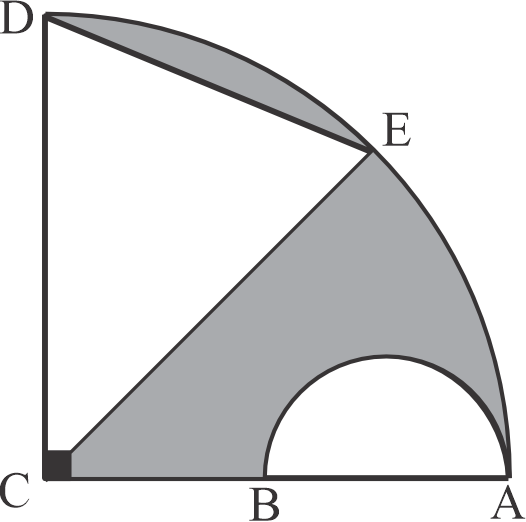
\includegraphics[width=3.2cm]{imagenes/CEPRE-UNA2024-I/etapa2/soc/rm4c24-I.png}
	\end{center}
	
	\begin{enumerate}[label=\alph*)]
		\item $(8+3\pi)\,cm$
		\item $(9+2\pi)\,cm$
		\item $(10+3\pi)\,cm$
		\item $\left(8+\dfrac{5\pi}{2}\right)\,cm$
		\item $(7+\pi)\,cm$
	\end{enumerate}
	\textbf{Respuesta correcta:} c)
	
	\vspace{2mm}
	\textbf{Solucionario:}\\[1mm]
	Como $AB=BC=2$, entonces $CA=4$ y el cuarto de circunferencia tiene radio $4$.
	
	Además, $CD=4$ y por dato $DE=4$.
	
	El arco total $\widehat{DA}$ del cuarto de circunferencia mide:
	
	$L_1=\dfrac{1}{4}(2\pi\cdot 4)=2\pi$.
	
	El semicírculo tiene radio $1$, así que su arco mide:
	
	$L_2=\pi$.
	
	Los segmentos rectos del contorno sombreado son $DE=4$, $CE=4$ y $CB=2$.
	
	Entonces el perímetro total es:
	
	$P=2\pi+\pi+4+4+2=$\fbox{$10+3\pi$}
	
	\vspace{6mm}
	
	\item Definimos el operador
	
	$\boxed{2x+1}=4x+7$
	
	Halle el valor de $\boxed{8}$
	\begin{enumerate}[label=\alph*)]
		\item 17
		\item 18
		\item 35
		\item 21
		\item 25
	\end{enumerate}
	\textbf{Respuesta correcta:} d)
	
	\vspace{2mm}
	\textbf{Solucionario:}\\[1mm]
	Sea $\boxed{y}=f(y)$.
	
	Dado que si $y=2x+1$, entonces:
	
	$f(y)=4x+7=2(2x+1)+5=2y+5$.
	
	Por tanto:
	
	$\boxed{8}=2(8)+5=$\fbox{$21$}
	
	\vspace{6mm}
	
	\item Determine $x+y$ si
	
	\begin{center}
		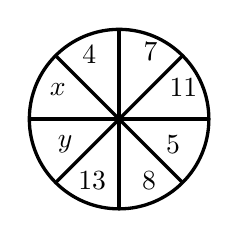
\begin{tikzpicture}[scale=0.38]
			\draw[very thick] (0,0) circle (3);
			
			\draw[very thick] (0,0) -- (0,3);
			\draw[very thick] (0,0) -- (2.12,2.12);
			\draw[very thick] (0,0) -- (3,0);
			\draw[very thick] (0,0) -- (2.12,-2.12);
			\draw[very thick] (0,0) -- (0,-3);
			\draw[very thick] (0,0) -- (-2.12,-2.12);
			\draw[very thick] (0,0) -- (-3,0);
			\draw[very thick] (0,0) -- (-2.12,2.12);
			
			\node at (1.05,2.25) {$7$};
			\node at (2.15,1.05) {$11$};
			\node at (1.8,-0.85) {$5$};
			\node at (1.0,-2.05) {$8$};
			\node at (-0.9,-2.05) {$13$};
			\node at (-1.8,-0.85) {$y$};
			\node at (-2.05,1.0) {$x$};
			\node at (-1.0,2.15) {$4$};
		\end{tikzpicture}
	\end{center}
	
	\begin{enumerate}[label=\alph*)]
		\item 17
		\item 18
		\item 20
		\item 24
		\item 26
	\end{enumerate}
	\textbf{Respuesta correcta:} e) 
	
	\vspace{2mm}
	\textbf{Solucionario:}\\[1mm]
	
	\begin{center}
		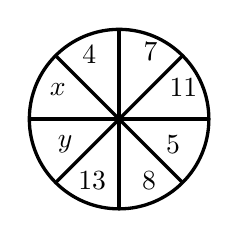
\begin{tikzpicture}[scale=0.38]
			\draw[very thick] (0,0) circle (3);
			
			\draw[very thick] (0,0) -- (0,3);
			\draw[very thick] (0,0) -- (2.12,2.12);
			\draw[very thick] (0,0) -- (3,0);
			\draw[very thick] (0,0) -- (2.12,-2.12);
			\draw[very thick] (0,0) -- (0,-3);
			\draw[very thick] (0,0) -- (-2.12,-2.12);
			\draw[very thick] (0,0) -- (-3,0);
			\draw[very thick] (0,0) -- (-2.12,2.12);
			
			\node at (1.05,2.25) {$7$};
			\node at (2.15,1.05) {$11$};
			\node at (1.8,-0.85) {$5$};
			\node at (1.0,-2.05) {$8$};
			\node at (-0.9,-2.05) {$13$};
			\node at (-1.8,-0.85) {$y$};
			\node at (-2.05,1.0) {$x$};
			\node at (-1.0,2.15) {$4$};
		\end{tikzpicture}
	\end{center}
	
	La suma de $4+7=11$ \\
	La suma de $11+5=16$ \\
	La suma de $8+13=21$\\
	La suma de $y+x=?$  \\
	
	
	$11,16,21,?$ la diferencia entre estas es 5 
	
	por lo tanto  $y+x=21+5=$\fbox{$26$}
	\vspace{6mm}
\end{enumerate}

\subsection*{Razonamiento Verbal}

\begin{enumerate}[resume]

	
	\item En la palabra \textbf{ABSTEMIO}, el prefijo \textbf{ABS} significa:
	\begin{enumerate}[label=\alph*)]
		\item condenación.
		\item construcción.
		\item separación.
		\item inferencia.
		\item relación.
	\end{enumerate}
	\textbf{Respuesta correcta:} c)
	
	\vspace{2mm}
	\textbf{Solucionario:}\\[1mm]
	El prefijo latino \textbf{abs-} expresa idea de alejamiento o \textbf{separación}.
	
	Por eso ``abstemio'' alude a quien se aparta de beber alcohol.
	

	
	\vspace{6mm}
	
	\item Para la universidad, la excelencia académica significa lograr una educación \rule{1cm}{0.15mm} forma profesionales competentes y éticos, \rule{1cm}{0.15mm} aporten al desarrollo del país.
	\begin{enumerate}[label=\alph*)]
		\item que - quienes
		\item cuando - mientras
		\item donde - pero
		\item cual - cuyos
		\item cuyo - más
	\end{enumerate}
	\textbf{Respuesta correcta:} a)
	
	\vspace{2mm}
	\textbf{Solucionario:}\\[1mm]
	La forma correcta es: ``una educación \textbf{que} forma profesionales competentes y éticos, \textbf{quienes} aporten al desarrollo del país''.
	

	
	\vspace{6mm}
	
	\item El antónimo de la palabra \textbf{ALEVOSÍA} es:
	\begin{enumerate}[label=\alph*)]
		\item felonía.
		\item perfidia.
		\item traición.
		\item condición.
		\item lealtad.
	\end{enumerate}
	\textbf{Respuesta correcta:} e)
	
	\vspace{2mm}
	\textbf{Solucionario:}\\[1mm]
	``Alevosía'' se relaciona con traición o perfidia; su antónimo es \textbf{lealtad}.
	

	
	\vspace{6mm}
	
	\item El sinónimo de la palabra \textbf{LACÓNICO} es:
	\begin{enumerate}[label=\alph*)]
		\item breve.
		\item enjuto.
		\item parco.
		\item agotado.
		\item caviloso.
	\end{enumerate}
	\textbf{Respuesta correcta:} a)
	
	\vspace{2mm}
	\textbf{Solucionario:}\\[1mm]
	``Lacónico'' significa breve, conciso, de pocas palabras.
	
	La opción más directa es \textbf{breve}.
	

	
	\vspace{6mm}
	
	\item \textbf{PLAN DE REDACCIÓN}
	
	I. Ahora que he ingresado, me toca estudiar para hacer realidad mi carrera.\\
	II. He concluido mi secundaria, soy uno de los 260 000 estudiantes que egresan cada año.\\
	III. De antemano, sé que la competencia es dura, por eso me he preparado a conciencia.\\
	IV. Deseo seguir mis estudios en una buena universidad, la mejor de todas.\\
	V. Di mi examen y respondí todas las preguntas que sabía.
	
	\begin{enumerate}[label=\alph*)]
		\item II -- IV -- I -- V -- III
		\item II -- III -- I -- IV -- V
		\item I -- II -- V -- IV -- III
		\item II -- IV -- III -- V -- I
		\item II -- IV -- I -- III -- V
	\end{enumerate}
	\textbf{Respuesta correcta:} d)
	
	\vspace{2mm}
	\textbf{Solucionario:}\\[1mm]
	El orden lógico es: primero concluye la secundaria (II), luego expresa su deseo de seguir estudios (IV), después reconoce la competencia y se prepara (III), luego da el examen (V) y finalmente, al ingresar, se proyecta a estudiar la carrera (I).
	

	
	\vspace{6mm}
	
	\item \textbf{COMPRENSIÓN DE TEXTO}
	
	\begin{quote}
		Soy otro cuando soy; los actos míos son más míos\\
		si son también de todos, para que pueda ser, he\\
		de ser otro, salir de mí, buscarme entre los otros.
	\end{quote}
	\hfill Octavio Paz
	
	¿Cuál es la intención del autor?
	\begin{enumerate}[label=\alph*)]
		\item Mostrarse como otro.
		\item Evitar ser confundido con los otros.
		\item Argumentar sobre la referencia colectiva del ser humano.
		\item Evidenciar las semejanzas entre unos y otros.
		\item Hablar sobre la identidad del hombre.
	\end{enumerate}
	\textbf{Respuesta correcta:} c)
	
	\vspace{2mm}
	\textbf{Solucionario:}\\[1mm]
	Octavio Paz argumenta que el individuo se realiza plenamente solo en relación con los demás.
	
	La frase \textit{``los actos míos son más míos si son también de todos''} evidencia que la intención central es destacar la \textbf{dimensión colectiva del ser humano} como condición necesaria para la identidad individual.
	

	
	\vspace{6mm}
\end{enumerate}

\subsection*{Inglés}

\begin{enumerate}[resume]

	
	\item Select the sentence with the irregular verb in simple past tense.
	\begin{enumerate}[label=\alph*)]
		\item Yesterday I bought a new book.
		\item Yesterday I worked very hard.
		\item Yesterday I studied until midnight.
		\item Yesterday I travelled to Juliaca.
		\item I missed you yesterday.
	\end{enumerate}
	\textbf{Respuesta correcta:} a)
	
	\vspace{2mm}
	\textbf{Solucionario:}\\[1mm]
	The verb \textit{bought} is the simple past of the irregular verb \textit{buy}.
	
	The others are regular past forms.
	

	
	\vspace{6mm}
	
	\item Choose the correct auxiliar verb to complete the next question:
	
	A. Where \rule{1.5cm}{0.15mm} she live?\\
	B. She lives in a small village.
	\begin{enumerate}[label=\alph*)]
		\item will
		\item do
		\item is
		\item does
		\item was
	\end{enumerate}
	\textbf{Respuesta correcta:} d)
	
	\vspace{2mm}
	\textbf{Solucionario:}\\[1mm]
	For third person singular in the simple present, the correct auxiliary is \textit{does}: ``Where \textbf{does} she live?''
	

	
	\vspace{6mm}
\end{enumerate}

\subsection*{Quechua y Aimara}

\begin{enumerate}[resume]

	
	\item ¿Hayk’a pachayuqtaq chawpi p’unchawri kan? / ¿Qawqha pachanisa chikata uruxa?
	\begin{enumerate}[label=\alph*)]
		\item Chunka iskayniyuq / Tunka paya pachani
		\item Iskay chunka iskayniyuq / Paya tunka paya pachani
		\item Iskay chunka tawayuq / Paya tunka pusi pachani
		\item Iskay chunka pichqayuq / Paya tunka phisqa pachani
		\item Iskay chunka suqtayuq / Paya tunka suxta pachani
	\end{enumerate}
	\textbf{Respuesta correcta:} a)
	
	\vspace{2mm}
	\textbf{Solucionario:}\\[1mm]
	La pregunta alude al \textbf{medio día}, es decir, 12 horas.
	
	En quechua corresponde a \textit{chunka iskayniyuq} y en aimara a \textit{tunka paya pachani}.
	

	
	\vspace{6mm}
	
	\item ¿Imatataq wallpakunari churanku? / ¿Kunsa wallpanakaxa uskampxi?
	\begin{enumerate}[label=\alph*)]
		\item Runtuta / K'awna
		\item Q’awata / Phaña
		\item Rumita / Qala
		\item Makita / Ampara
		\item Muhuta / Jatha
	\end{enumerate}
	\textbf{Respuesta correcta:} a)
	
	\vspace{2mm}
	\textbf{Solucionario:}\\[1mm]
	La gallina pone \textbf{huevos}.
	
	En quechua es \textit{runtu}; la pareja correcta en la opción es la \textbf{a)}.
	

	
	\vspace{6mm}
\end{enumerate}



\newpage

\section*{Ejercicios Propuestos}

\addcontentsline{toc}{subsection}{Ejercicios Propuestos}

\begin{enumerate}
	
	\item Se tiene el número $8abc$ que al dividirlo entre 37 da un residuo de 4. ¿Cuál es el residuo al dividir el número $abc4$ entre 37?
	\begin{enumerate}[label=\Alph*)]
		\item 4
		\item 5
		\item 2
		\item 3
		\item 1
	\end{enumerate}
	
	\item De las siguientes proposiciones, ¿cuáles son equivalentes entre sí?
	
	I. Pedro no va a la fiesta porque estudia para su examen.\\
	II. Pedro no estudia para su examen y no va a la fiesta.\\
	III. No es cierto que Pedro estudie para su examen y vaya a la fiesta.\\
	IV. Pedro va a la fiesta y no estudia para su examen.
	
	\begin{enumerate}[label=\Alph*)]
		\item III y IV
		\item II y III
		\item I y II
		\item I y III
		\item II y IV
	\end{enumerate}
	
	\item Sea $A$ una matriz cuadrada de orden $3\times 3$ con $\det(A)=-4$. Calcular el valor de $\det(2A^T(A^2)^{-1})$.
	\begin{enumerate}[label=\Alph*)]
		\item $-4$
		\item 3
		\item $-2$
		\item $-3$
		\item 4
	\end{enumerate}
	
	\item Halle $m+n$ si al dividir:
	
	$\dfrac{2x^4+x^3+3x^2+mx+n}{x^2-2x+1}$
	
	se obtiene como resto $7x+5$.
	
	\begin{enumerate}[label=\Alph*)]
		\item 4
		\item 5
		\item 7
		\item 3
		\item 1
	\end{enumerate}
	
	\item Un postulante de la UNA Puno observa la maqueta de un parque. Si desea colocar un reflector en el segmento $AC$, lo más próximo al reflector ubicado en $B$, ¿a qué distancia de $B$ lo colocará si se sabe que $AC=28$ cm?
	
	\begin{center}
		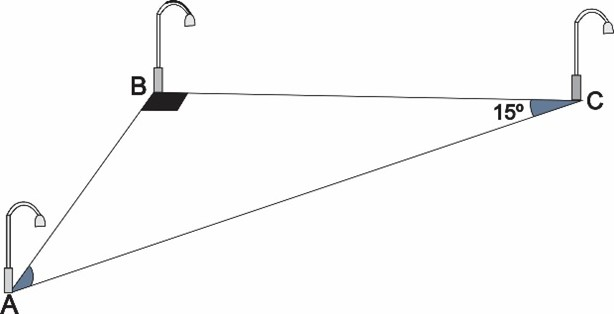
\includegraphics[width=4.5cm]{imagenes/propuestos/geo3.png}
	\end{center}
	
	\begin{enumerate}[label=\Alph*)]
		\item 7 cm
		\item 8 cm
		\item 4 cm
		\item 5 cm
		\item 6 cm
	\end{enumerate}
	
	\item Un paralelogramo $ABCD$, $AB=3$, $BC=5$, $AC=7$. Calcule $m\angle A$.
	\begin{enumerate}[label=\Alph*)]
		\item $120^\circ$
		\item $20^\circ$
		\item $10^\circ$
		\item $25^\circ$
		\item $53^\circ$
	\end{enumerate}
	
	\item En un triángulo rectángulo, uno de los ángulos agudos mide $\dfrac{2\pi}{5}$ rad. Determine el otro ángulo agudo en el sistema sexagesimal.
	\begin{enumerate}[label=\Alph*)]
		\item $-62^\circ$
		\item $73^\circ$
		\item $18^\circ$
		\item $45^\circ$
		\item $26^\circ$
	\end{enumerate}
	
	\item En la figura, determina $\tan\theta$.
	
	\begin{center}
		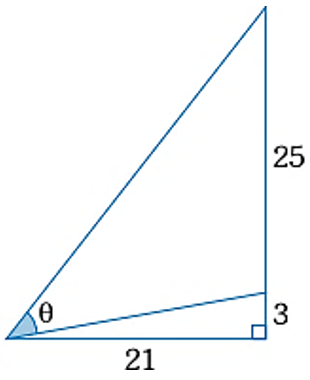
\includegraphics[width=2cm]{imagenes/propuestos/trigo4.png}
	\end{center}
	
	\begin{enumerate}[label=\Alph*)]
		\item $2\sqrt{3}$
		\item 1
		\item 2
		\item 5
		\item 24
	\end{enumerate}
	
	\item Un bloque de 10 kg de masa está sobre el plano inclinado como se muestra en la figura. Determine el tiempo que demora el bloque en llegar a la base del plano. El coeficiente de fricción entre el bloque y el plano es 0,5. $(g=10\ \text{m/s}^2)$
	
	\begin{center}
		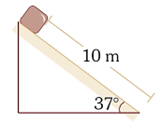
\includegraphics[width=3cm]{imagenes/propuestos/fisica3.png}
	\end{center}
	
	\begin{enumerate}[label=\Alph*)]
		\item $2\sqrt{10}$ s
		\item 4 s
		\item $2\sqrt{5}$ s
		\item $\sqrt{5}$ s
		\item $\sqrt{10}$ s
	\end{enumerate}
	
	\item Qué tiempo debe circular una corriente eléctrica de 10 A por una resistencia de 4,2 $\Omega$ para que con el calor disipado se logre elevar la temperatura de 480 g de agua de $40^\circ$C a $50^\circ$C. $(1\ \text{cal}=4,2\ \text{J})$
	\begin{enumerate}[label=\Alph*)]
		\item 48 s
		\item 480 s
		\item 4,8 s
		\item 12,1 s
		\item 24,0 s
	\end{enumerate}
	
	\item Indica verdadero (V) o falso (F), según corresponda respecto a los isótopos.
	
	I. Son átomos que tienen propiedades químicas idénticas.\\
	II. Son átomos que tienen propiedades físicas diferentes.\\
	III. Todo elemento posee dos o más isótopos naturales, además de ser estables.\\
	IV. Poseen diferente número de nucleones fundamentales.\\
	V. El isótopo más abundante en la naturaleza es el de menor número de masa.
	
	\begin{enumerate}[label=\Alph*)]
		\item FVVFF
		\item VVFVV
		\item FFVFF
		\item FFFVV
		\item VFVVV
	\end{enumerate}
	
	\item Elija tres metales pesados que causan mayor preocupación ecológica.
	\begin{enumerate}[label=\Alph*)]
		\item Hg, As, Li
		\item Pb, Hg, Ag
		\item Hg, Na, Au
		\item Hg, Pb, As
		\item Pb, As, Ag
	\end{enumerate}
	
	\item Entre los músculos de la masticación se encuentra el masetero, cuyo origen es el:
	\begin{enumerate}[label=\Alph*)]
		\item ala mayor de la apófisis pterigoides.
		\item ala menor de la apófisis pterigoides.
		\item borde inferior del hueso parietal.
		\item borde inferior del arco cigomático.
		\item borde inferior de la apófisis pterigoides.
	\end{enumerate}
	
	\item Una de las alternativas corresponde a los trastornos autosómicos dominantes del sistema esquelético.
	\begin{enumerate}[label=\Alph*)]
		\item Neurofibromatosis
		\item distrofia miotónica
		\item síndrome de Marfan
		\item enfermedad de Huntington
		\item borde inferior de la apófisis pterigoides.
	\end{enumerate}
	
	\item Un tema fundamental en la filosofía se refiere al problema relacionado al ser, es decir, determinar qué es primero en la relación ser-pensar. Esta problemática es desarrollada por la rama de la filosofía denominada:
	\begin{enumerate}[label=\Alph*)]
		\item Ontología
		\item Epistemología
		\item Lógica
		\item Idealismo
		\item Metafísica
	\end{enumerate}
	
	\item El saber en general es el conjunto de conocimientos adquiridos por el hombre. El conocimiento científico inicia con el saber:
	\begin{enumerate}[label=\Alph*)]
		\item Espontáneo
		\item Filosófico
		\item Trascendente
		\item Común
		\item Formal
	\end{enumerate}
	
	\item La siguiente descripción: “Se divide en dos sectores, la rama costera y oceánica, transportan entre $40^\circ S$ y $45^\circ S$ masas de agua, son de baja salinidad, alto contenido de oxígeno disuelto, que le permite generar mejores condiciones para la vida marina”; nos referimos a:
	\begin{enumerate}[label=\Alph*)]
		\item La corriente del Niño
		\item La corriente Oceánica
		\item La corriente de Humboldt
		\item La contracorriente del Perú
		\item La corriente Submarina
	\end{enumerate}
	
	\item Las siguientes subcuencas como las de Inambari, Tambopata, Orthon, Las Piedras; pertenecen a la cuenca hidrográfica del río:
	\begin{enumerate}[label=\Alph*)]
		\item Marañón
		\item Ucayali
		\item Madre de Dios
		\item Huallaga
		\item Napo
	\end{enumerate}
	
	\item Las asimetrías entre ricos y pobres en el Perú denotan la forma de violencia denominada:
	\begin{enumerate}[label=\Alph*)]
		\item Estructural
		\item Política
		\item micro social
		\item natural
		\item étnica-cultural
	\end{enumerate}
	
	
		\item Son representantes de la escuela neoliberal.
	
	1. John Keynes\\
	2. Von Hayeck\\
	3. Margaret Thacher\\
	4. Ronald Reagan\\
	5. David Ricardo
	
	Son ciertas:
	\begin{enumerate}[label=\Alph*)]
		\item 1, 2 y 5
		\item 1, 3 y 4
		\item 1, 4 y 5
		\item 3 y 4
		\item 3 y 5
	\end{enumerate}
	
	\item Marque verdad (V) o falsedad (F) en relación con el sistema financiero.
	
	1. Un acreedor financiero es una empresa que obtiene préstamo.\\
	2. La tasa activa y pasiva normalmente son iguales.\\
	3. Una caja rural pertenece al sistema financiero directo.
	
	\begin{enumerate}[label=\Alph*)]
		\item FFF
		\item FVV
		\item VVV
		\item VFF
		\item VVF
	\end{enumerate}
	
	\item Es una característica propia del arcaico superior o de los horticultores sedentarios en la Historia del Perú:
	\begin{enumerate}[label=\Alph*)]
		\item la presencia de la cunicultura
		\item las técnicas de percusión y presión para el tallado de la piedra
		\item la construcción de los primeros centros ceremoniales
		\item la formación de las primeras aldeas
		\item la primera domesticación del perro
	\end{enumerate}
	
	\item Uno de los enunciados no corresponde a la Carta a los Españoles Americanos.
	\begin{enumerate}[label=\Alph*)]
		\item Es un documento de tendencia separatista.
		\item Fue redactado por Juan Pablo Vizcardo y Guzmán.
		\item La versión original fue en francés.
		\item Promueve la idea de patria continental.
		\item Rechaza la presencia de las tropas napoleónicas en España.
	\end{enumerate}
	
	\item El primero en fundamentar que el temor del hombre, por ser antisocial, ha hecho necesario el surgimiento del Estado como autoridad omnipotente e incontrastable, es:
	\begin{enumerate}[label=\Alph*)]
		\item Rousseau
		\item Sócrates
		\item Platón
		\item Hobbes
		\item Aristóteles
	\end{enumerate}
	
	\item En los versos de “Los Reyes Rojos” de Eguren: “Por verde bosque / Y en los purpurinos cerros / Vibra su ceño. // Falcones reyes / Batallan en lejanías / De oro de azulinas // Por la luz cadmio, / Airadas se ven pequeñas, / sus formas negras...”, la influencia de los movimientos literarios son:
	\begin{enumerate}[label=\Alph*)]
		\item sinestesia -- simbolismo
		\item creacionismo -- modernismo
		\item simbolismo -- parnasianismo
		\item pre modernismo -- futurismo
		\item tradicionalismo - esteticismo
	\end{enumerate}
	
	\item El texto: “Aguacero, aguacerito / Granizadita, granizadita / mira, no me mojes / no me granices / tengo manta corta / tengo poncho chico”, corresponde a un:
	\begin{enumerate}[label=\Alph*)]
		\item Aymoray
		\item Coyllur
		\item Arawy
		\item Urpi
		\item Huakatapi
	\end{enumerate}
	
	\item El número de términos que tiene la serie:
	
	$9,\ 12,\ 15,\ 16,\ 21,\ 20,\ \ldots,\ 64$
	
	es:
	
	\begin{enumerate}[label=\Alph*)]
		\item 28
		\item 29
		\item 30
		\item 31
		\item 32
	\end{enumerate}
	
	\item En un examen para ingreso a una Universidad, un postulante comentaba: “De las 80 preguntas formuladas, si hubiera contestado solo la tercera parte de las preguntas que he contestado habría contestado menos de 17 preguntas; además, el triple de las preguntas que no contesté es menor que el doble de preguntas que contesté, disminuido en 5”. La cantidad de preguntas que no contestó el postulante fue:
	\begin{enumerate}[label=\Alph*)]
		\item 10
		\item 30
		\item 50
		\item 52
		\item 54
	\end{enumerate}
	
	\item Elegir la alternativa que contenga el vocablo con el significado antónimo absoluto contextual, respecto del que posee el término subrayado en el enunciado siguiente:
	
	\textit{Es capaz de aglutinar a la gente más dispar.}
	
	\begin{enumerate}[label=\Alph*)]
		\item Unir
		\item Junta
		\item Separar
		\item Extraviar
		\item alentar
	\end{enumerate}
	
	\item Localizar en el texto la idea principal y determinar qué tipo de párrafo es por su ubicación. Texto base:
	
	\textit{Se entiende por libertad a aquella capacidad de autodeterminación de la voluntad, que permite a los seres humanos actuar como deseen. En tal sentido, suele ser denominada libertad individual. El término libertad se vincula a la soberanía de su país en la vertiente de “libertad nacional”. Aunque desde esta perspectiva tradicional, la libertad puede ser civil o política, el concepto moderno incluye un conjunto general de derechos individuales, como la igualdad de oportunidades o el derecho a la educación. Pese a todas estas particularidades históricas se conserva aquella parte esencial de su definición que afirma que libertad es la autonomía de la voluntad a partir de la cual el hombre actúa como mejor le venga en gana.}
	
	\begin{enumerate}[label=\Alph*)]
		\item Encuadrado
		\item Paralelo
		\item Analizante
		\item alternado-centrado
		\item sintetizante
	\end{enumerate}
	
	\item “Yachachiq” simipi, “-q” sufijochasqa ima nirqan?
	\begin{enumerate}[label=\Alph*)]
		\item Mana
		\item Runa
		\item Riqsi
		\item Runapas hina ruwachiq
		\item Tinkuy
	\end{enumerate}
	
	\item ¿Imanallataq “viernes” nisqaqa?
	\begin{enumerate}[label=\Alph*)]
		\item K’anchay
		\item Viernesmanta
		\item Ch’askimanta
		\item Ch’isi
		\item Killachay
	\end{enumerate}
	

	
	\item The boy \_\_\_ won the race is my cousin.
	\begin{enumerate}[label=\Alph*)]
		\item which
		\item where
		\item who
		\item whom
		\item that whom
	\end{enumerate}
	
	\item She usually studies \_\_\_ night.
	\begin{enumerate}[label=\Alph*)]
		\item in
		\item at
		\item on
		\item to
		\item by
	\end{enumerate}
	
	\end{enumerate}




\subsubsection*{Claves de Respuestas}


\begin{center}
	\begin{tabular}{ll ll ll ll ll ll}
		1) E & 2) D & 3) C & 4) C & 5) A & 6) A \\
		7) C & 8) B & 9) E & 10) A & 11) B & 12) D \\
		13) D & 14) C & 15) A & 16) A & 17) C & 18) C \\
		19) A & 20) A & 21) C & 22) E & 23) D & 24) C \\
		25) A & 26) A & 27) B & 28) C & 29) A & 30) D \\
		31) B & 32) C & 33) B & 34) B & & \\
	\end{tabular}
\end{center}

